%Here you can change the paper and mche the trims to appear

\def\papersize    {b5paper} % Final papersize (b5paper/a4paper), recommended papersize for DTU is b5paper
\def\showtrims    {false} % Print on larger paper than \papersize and show trim marks (true/false)?
\def\confidential {false} % Confidential thesis (true/false)?


\input{preamble/general}
\usepackage{fontspec}

% Sans-serif font
\setsansfont[
    Ligatures=TeX,
    Extension=.otf,
    UprightFont=*-regular,
    BoldFont=*-bold,
    ItalicFont=*-italic,
    BoldItalicFont=*-bolditalic,
    %SlantedFont=,
    %BoldSlantedFont=,
    %SmallCapsFont=
    Scale=0.8      % Adjustmens when using math in sections
]{texgyreadventor}


\input{preamble/etc}


%used packages 
\usepackage{pdflscape}

 \usepackage{titlesec}


% \titleformat{\paragraph}
% {\normalfont\normalsize\bfseries}{\theparagraph}{1em}{}
% \titlespacing*{\paragraph}
% {0pt}{3.25ex plus 1ex minus .2ex}{1.5ex plus .2ex}
%\setcounter{secnumdepth}{5}

\usepackage{amsmath}
\usepackage{tikz}
\usetikzlibrary{shapes,arrows}
% Define block styles
\tikzstyle{decision} = [diamond, draw, fill=white!20, 
    text width=4.5em, text badly centered, node distance=3cm, inner sep=0pt]
\tikzstyle{block} = [rectangle, draw, fill=white!20, 
    text width=10em, text centered, rounded corners, minimum height=4em]
\tikzstyle{line} = [draw, -latex']
\tikzstyle{cloud} = [draw, ellipse,fill=white!20, node distance=3cm,
    minimum height=2em]
\usetikzlibrary{backgrounds,fit}
\usepackage{pgfplots}
\pgfplotsset{compat=1.15}
\usepackage{mathrsfs}
\usetikzlibrary{arrows}
\usepackage{svg}

%% package alg 
\usepackage{fancyhdr,graphicx,amsmath,amssymb}
\usepackage[ruled,vlined,linesnumbered]{algorithm2e}



%% numbreing paragraphs 

\newcommand*\numcircledmod[1]{\raisebox{.5pt}{\textcircled{\raisebox{-.9pt} {#1}}}}

% mini TOC 
\usepackage{minitoc}
\usepackage{amsthm}
\usepackage{graphicx}
\usepackage{fancyhdr}
\usepackage{enumerate}
\usepackage{natbib}
\usepackage{url}
\usepackage{paralist}
\bibliographystyle{plain}
\usepackage{blindtext}
\usepackage{amssymb}
%\usepackage{minitoc}
\usepackage{makeidx}
%\title{\textbf{Teoria degli insiemi:\\variabili e domini di quantificazione}}
%\author{\textit{Bla Bla}\\Università Bla bla \vspace*{-0.25cm}\\ Cdl in bla\vspace*{-0.25cm}\\bla bla}

\usepackage{etoc}
\etocsettocstyle{}{}%

\usepackage{empheq}


\usepackage{listofitems,environ}
\usepackage{geometry}
%\usepackage[dvipsnames]{xcolor}
% \usepackage{hyperref}

% % \definecolor{mycolor}{HTML}{F7F8E0}
% % \definecolor{myorange}{RGB}{245,156,74}

% \hypersetup{
%   colorlinks=true,
%   urlcolor=blue
% }

\usepackage{epigraph} 


\begin{document}
\clearforchapter

\frontmatter

%\prefrontmatter

\newgeometry{%
    paper = a4paper,%
    top = 40pt,%
    hmargin = 58pt,%
    bottom = 40pt,%         <---- Changing this has no effect
    headsep = 50pt,%
}


\thispagestyle{empty}             % No page numbers

\begin{titlingpage}
    \begin{center}
        \vspace*{1cm}
        \textbf{\LARGE Safe and Energy Efficient Decision/Control Architecture for a Formation of Multi-Vehicle 
        System in Dynamic Environment}

        
        \vspace{0.3cm}
        {\normalsize by}

        
        \vspace{0.3cm}
        {\large Lyes SAIDI}

        \vspace{0.5cm}
        {\large \textbf{Specialty: Automatics \& Robotics}}

        \vspace{0.5cm}
        {\large PhD defense on January 10, 2024. In front of the jury composed of:}
        \vspace{0.2cm}

        \hline
        \vspace{0.2cm}

       \textbf{Reviewers}
        \vspace{0.2cm}

\begin{tabular}{c c}
     \textit{Michel BASSET}      & \textit{Philippe MARTINET} \\
     Professeur des Universités   & Directeur de recherche \\
     Univ. Haute-Alsace           & Inria Sophia Antipolis
\end{tabular}
        \vspace{0.5cm}

       \textbf{Examiners}
        \vspace{0.2cm}

\begin{tabular}{c c}
     \textit{ Olivier SIMONIN}          & \textit{Maan EL BADAOUI EL NAJJAR}  \\
     Professeur des Universités        & Professeur des Universités          \\
     INSA Lyon, Univ. de Lyon          & CRIStAL, Univ. de Lille                     
\end{tabular}

        \vspace{0.2cm}

\begin{tabular}{c }
         \textit{Véronique CHERFAOUI} \\
         Professeure des Universités \\
         Heudiasyc, UTC  
\end{tabular}

        \vspace{0.5cm}


       \textbf{Supervisors}
        \vspace{0.2cm}

\begin{tabular}{c c}
     \textit{Lounis ADOUANE}                           & \textit{Reine TALJ} \\
     Professeur des Universités                        & Chargée de Recherche CNRS, HDR \\
     Heudiasyc, UTC                                    & Heudiasyc, UTC
\end{tabular}


        % \begin{tabular}{lll}
        %     \textbf{Reviewers}   & Romuald Aufrère     & Univ. Clermont Auvergne \\
        %                          & Rémi Boutteau       & Univ. de Rouen Normandie \\
        %     \textbf{Examiners}   & Franck Davoine      & Univ. de Technologie de Compiègne \\
        %                          & Joelle Hage         & Univ. de Technologie de Compiègne \\
        %                          & Fawzi Nashashibi    & Inria Paris Rocquencourt \\
        %                          & Clément Zinoune     & Renault \\
        %     \textbf{Supervisors} & Philippe Bonnifait  & Univ. de Technologie de Compiègne \\
        %                          & Véronique Cherfaoui & Univ. de Technologie de Compiègne \\
        % \end{tabular}
        \vspace{0.2cm}

        \hline



        \vspace{0.5cm}
        {\Large PhD Thesis prepared at the Heudiasyc Laboratory, UMR UTC/CNRS 7253}

        
        \vspace{1cm}\hfill
        \includegraphics[height=0.06\textheight]{prefrontmatter/utc.png}\hfill
        \includegraphics[height=0.06\textheight]{prefrontmatter/Logo_Heudiasyc.png}\hfill
        \includegraphics[height=0.06\textheight]{prefrontmatter/cnrs.png}\hfill
    \end{center}
\end{titlingpage}



\restoregeometry
%\cleartoevenpage
\cleardoublepage

%%!TEX root = ../Thesis.tex
\thispagestyle{empty} % No page numbers
\frieze
\noindent
\sffamily

\large
\vspace*{\fill}
\hspace{-0.52cm}\textbf{Supervisor:} Prof. Sergio Leone\\
\textbf{Co-supervisors:} Prof. John Wayne \& Ass. Prof. Clint Eastwood
\vspace{5cm}

\small
% Leave the following empty spaces to avoid the Warning: "Underfull \hbox (badness 10000)"
\hspace*{\fill}\textbf{DTU Fotonik}

\hspace*{\fill}\textbf{Department of Photonics Engineering}

\hspace*{\fill}\textbf{Technical University of Denmark}

\hspace*{\fill}Ørsteds Plads

\hspace*{\fill}Building 340

\hspace*{\fill}2800 Kongens Lyngby, Denmark


\normalsize
\normalfont
\vspace*{2cm}

\clearforchapter

\frontmatter

\newgeometry{%
    paper = a4paper,%
    top = 5pt,%
    hmargin = 58pt,%
    bottom = 60pt,%         <---- Changing this has no effect
    headsep = 50pt,%
}


\include{frontmatter/Summary}
\restoregeometry
\clearforchapter

\frontmatter
\newgeometry{%
    paper = a4paper,%
    top = -10pt,%
    hmargin = 58pt,%
    bottom = 40pt,%         <---- Changing this has no effect
    headsep = 50pt,%
}

\chapter{Résumé}
        \vspace{-0.2cm}
\thispagestyle{empty}

L'engouement important pour  les systèmes de transport intelligent est justifié principalement par l'impératif de réduire, voire annihiler, les erreurs humaines induisant les accidents. Cependant, s'attaquer uniquement aux Véhicules Autonomes (VAs) ``individuels'' demeure insuffisant, étant donné que plusieurs situations nécessitent la ``coordination'' des mouvements relatifs des VAs. Dans le paradigme du Système Multi-Véhicules (SMV), les VAs bénéficient de l'information issue de leur connectivité. Par conséquent, ils peuvent détecter plus précisément, traiter davantage d'informations et être contrôlés de manière plus précise. L'évaluation collaborative de la sécurité au sein du SMV permet l'établissement de stratégies avancées en matière d'évitement de collision, en particulier dans des scénarios complexes tels que les croisements au sein d'intersections et les insertions sur les entrées d'autoroute. De plus, la technologie SMV facilite la réduction des espaces entre les véhicules, améliorant ainsi la capacité et la fluidité du trafic routier. Le temps de réponse plus court du SMV permet un meilleur contrôle de la dynamique des VAs, ouvrant la voie à des stratégies énergétiques prometteuses. L'objectif principal des travaux de recherche constituant ce manuscrit de doctorat est de proposer une architecture de décision/contrôle sûre et peu énergivore pour le SMV naviguant dans des environnements dynamiques et complexes. Inspirée des architectures multi-contrôleurs, une Architecture Multi-Contrôleurs Coopérative est proposée. La première partie de l'architecture proposée concerne le niveau de prise de décision. Ce niveau, impliquant une stratégie de prise de décision à plusieurs comportements, est responsable de l'activation du comportement approprié du SMV en fonction de la métrique de sécurité. Deux comportements distincts sont proposés : (a) Le comportement nominal, conçu pour réaliser le scénario d'insertion tout en respectant les objectifs individuels des véhicules formant le SMV, est activé lorsqu'aucun risque de collision est détecté, (b) Le comportement coopératif est activé par le niveau de prise de décision lorsque l'exigence de sécurité n'est pas satisfaite par le comportement nominal. Son objectif est de résoudre le conflit lors de l'insertion en générant un ordre de passage sûr et économe énergétiquement pour les véhicules composant le SMV dans la zone d'insertion. La deuxième partie de l'architecture proposée se concentre sur le niveau de planification de trajectoire locale. Chaque comportement se voit attribuer un contrôleur dédié, conçu pour répondre à ses besoins spécifiques. Par exemple, le contrôleur du comportement coopératif est chargé de traduire l'ordre de passage des véhicules en dynamiques réalisables (trajectoire, vitesse, etc.). Cette tâche d'obtention de dynamiques réalisables est facilitée par la stratégie de reconfiguration dynamique de la formation proposée. En substance, l'approche tire parti des capacités de navigation en formation du SMV pour conceptualiser des manœuvres coopératives ayant trait d'insertion en milieu autoroutier, comme un problème de reconfiguration de formation. Une formalisation du problème de reconfiguration de la formation est présentée, utilisant une approche formelle, flexible et générique. La stratégie proposée utilise des cibles dynamiques virtuelles pour garantir une reconfiguration sécurisée de la formation, ceci, de sa forme initiale vers la configuration souhaitée par rapport à l'ordre de passage sélectionné. La performance de l'architecture globale a été évaluée par co-simulation en utilisant Matlab/Simulink et SCANeR studio.
        \vspace{-0.3cm}

 \paragraph*{ Mots-clés :}  Navigation coopérative en milieu autoroutier, Système multi-véhicules, Architecture multi-contrôleurs, Stratégie multi-comportementales de prise de décision, Stratégie de reconfiguration dynamique d'une formation.
 \clearpage
\restoregeometry



%%!TEX root = ../Thesis.tex

\chapter{Preface}
\blindtext[2]

\vfill

{
\centering
    Kongens Lyngby, \mydate\today\\[.5cm]
    \includegraphics[scale=0.2]{graphics/Signature.pdf}\\[.5cm]
\begin{center}
    Ross Moss
\end{center}
}
\thispagestyle{empty}



\vspace*{\fill} \epigraph{\itshape Comme tant de femme avant - et comme tant d'autres aujourd'hui encore -, elle n'a jamais eu de voyage à elle. J'aurais tellement voulu qu'elle puisse suivre la voie qu'elle aimait.}{My life on the road \\ Gloria Steinem \\ \itshape \textbf{A ma maman}}
\vfill\clearpage

\thispagestyle{empty}



\vspace*{\fill} \epigraph{\itshape Peu importe qui nous sommes et où nous vivons, tout au fond, nous nous sentons tous incomplets. C'est comme avoir perdu quelque chose et éprouver la nécessité de le retrouver. Quel est ce "quelque chose" ? La plupart d'entre nous ne le découvrirons jamais. Et parmi ceux qui y parviennent, plus rares encore sont ceux qui partent à sa quête.}{Soufi, mon amour \\ Elif Shafak \\ \itshape \textbf{A ma chérie}}
\vfill\clearpage



\thispagestyle{empty}

\chapter{Acknowledgements}


Firstly, I would like to express my gratitude to my thesis advisors, Reine Talj and Lounis Adouane, for their patience, assistance, and the relevance of their guidance. A PhD thesis is a somewhat adventurous experience, with an uncertain outcome; and it is partially thanks to them that I have completed mine.

I am also thankful to Philippe Martinet and Michel Basset for the honor of reviewing this dissertation, as well as to Véronique Cherfaoui and Olivier Simonin, who graciously agreed to contribute their efforts. I must not forget Maan El Badaoui El Najjar, who chaired the committee for my defense. I thank them all for their remarks and constructive criticisms.

Of course, I am grateful to all the fellow colleagues I have encountered during this thesis, in alphabetical order: Emmanuel Alao, Joelle Al Hage, Stéphane Bonnet, Maxime Escourrou, Chan He, Remy Huet, Antoine Lima, and Lahcene Mezouari.

The work presented in this dissertation is the result of three years of effort within the Heudiasyc laboratory, in the Computer Science Department of UTC. I wish to express my gratitude to all the members who contribute to making the work more enjoyable: my laboratory mates, the secretaries, and members of the logistics team, whose assistance I have appreciated.

Lastly, I extend my appreciation to the people who share my 6 pm to 11 pm, the fellow climbers from l'Association des Grimpeurs Compiégnois, Pauline, Emeline, Gérome, and all the other climbers. I am profoundly grateful to share my adventures with Maxime Noizet, Kiryan Devigne, and all my friends; their continuous support during these experiences was a game-changer. I thank my sister and brother for their unconditional care and kindness. To my beloved partner in crime, the being of light that inspires me to always push myself further. And to my beloved mother, my ocean of kindness.
 \clearpage
\cleardoublepage
\thispagestyle{empty}

%% TOC 
 \clearforchapter
 \phantomsection % This is added to make hyperref point to the right "Contents" page

 
 % \addcontentsline{toc}{part}{Contents} % Adds "Contents" as part-style in ToC
 %   \pagestyle{myruled} %Restores the heading style as before "appruled". Remove if "appruled" is commented

\include{frontmatter/Contents}



%% List of figures + tables 
\include{frontmatter/ListeOfFigures}
\include{frontmatter/ListeOfTables}

%% List of publication 
\newgeometry{%
    paper = a4paper,%
    top = 60pt,%
    hmargin = 58pt,%
    bottom = 60pt,%         <---- Changing this has no effect
    headsep = 50pt,%
}
\chapter{List of Publications}




\section*{International congress with proceedings}
\begin{itemize}
\item \hypertarget{ITSC23}{[ITSC’23]} Lyes Saidi, Reine Talj and Lounis Adouane, \textit{On-ramp Merging on Highway for Cooperative Automated Vehicles based on an Online Reconfigurable Formation Control Approach}. IEEE International Conference on Intelligent Transportation Systems, 24th-28th September 2023, In Bilbao, Spain. 



\item \hypertarget{MMAR23}{[MMAR'23]} Lyes Saidi, Lounis Adouane and Reine Talj. \textit{Altruistic Coordination Strategy for On-Ramp Merging on Highway of a Formation of Cooperative Automated Vehicles}. International Conference on Methods and Models in Automation and Robotics, 22th-27th August 2023, In Międzyzdroje, Poland. 


\item \hypertarget{ITSC22}{[ITSC’22]} Lyes Saidi, Lounis Adouane and Reine Talj, \textit{CORM: Constrained Optimal Reconfiguration Matrix for Safe On-Ramp Cooperative Merging of Automated Vehicles}. IEEE International Conference on Intelligent Transportation Systems, from 18th September to 18th October 2022, In Macau, China. 
\end{itemize}







\section*{International congress}
\begin{itemize}
    \item \hypertarget{VAMS23}{[VAMS’23]} Lyes Saidi, Lounis Adouane and Reine Talj, \textit{Cooperative Decision-Making for Safe On-Ramp Merging on Highway for Connected Automated Vehicles}. International Symposium on the Verification of Autonomous Mobile Systems, 9th-10th March 2023, In Paris, France.
\end{itemize}




\section*{National congress}

\begin{itemize}
    \item \hypertarget{CTATT22}{[CT ATT’22]} Lyes Saidi, Lounis Adouane and Reine Talj, \textit{Safe and Smooth On-ramp Merging on Highway Strategy for Cooperative Automated Vehicles}. Journées du Comité Technique Automatique et Transport Terrestre, 5th-6th April 2022, In Valenciennes, France. 

    \item \hypertarget{JJCR21}{[JJCR21]} Lyes Saidi, Lounis Adouane and Reine Talj, \textit{Toward a Robust and Safe Cooperative Highway Navigation of Multi-Vehicles Systems}. Journée des Jeunes Chercheurs en Robotique, 12th October 2021, In Paris, France.
\end{itemize}




\restoregeometry


\clearforchapter
\mainmatter


%% Acrtonyms 
%\chapter{Abbreviations}

\begin{acronym}[AVLAFTTT] % The name in the option ([...]) indicates the longest acronym to which the rest must align
\acro{A}{AAAAAAAAAAAAAAA}

\end{acronym}













% CORE of the manuscript 
  %!TEX root = ../Thesis.tex

\chapter*{General Introduction}
\addcontentsline{toc}{part}{General introduction} % Adds "Introduction" as part-style in ToC
\markboth{Introduction}{General introduction}    % Marks left and right headers as "Introduction"



\section*{1.\, \,  Context of the PhD thesis}

The transportation systems have provided humanity invaluable social and financial benefits, yet they are also intricately linked to adverse outcomes. The widespread use of automobile, while offering convenience, has given rise to challenges such as traffic congestion and an increase in traffic accidents. The investigation of accident causes has been a focal point of rigorous research for many years. According to \cite{humanerrors}, about $85\%$ of accidents can be attributed to human errors. Within this percentage, over $50\%$ are linked to decision errors, wherein drivers receive all relevant environment information but either refrain from making a decision, or choose an incorrect course of action. The remaining $35\%$ is attributed to inattention errors, where drivers are distracted, fail to respond, or lose control of their vehicles. 

A promising avenue to mitigate the majority of human errors is through the automation of the driving tasks. In recent years, the development of fully autonomous vehicles (AVs) for transportation has garnered significant attention from various researchers and industrials globally \cite{duarte2018impact}\cite{rosique2019systematic}\cite{schwarting2018planning}. The fundamental aim of autonomous vehicles is to surpass human perceptions of safety and judgment, particularly in perilous situations, and to produce appropriate actions \cite{dimiathesis}. Driving, being a complex task, demands the autonomous vehicle's ability to make critical decisions, achieved through various intra-vehicle process (e.g., situation awareness and assessment, decision-making, etc.). Moreover, an autonomous vehicle operates within a dynamic driving environment, alongside other road users, adding complexity to the driving task. 


The predominant focus of current autonomous vehicle research revolves around enabling \textit{individual} autonomous vehicles to navigate roads safely. However, there is a growing acknowledgment that to take fully advantage from the benefits of autonomous vehicle technology, certain scenarios will require the \textit{coordination} of relative activities and movements \cite{6949576}. An intriguing area of research is autonomous navigation with a group of vehicles, known as Multi-Vehicle System (MVS). The advantages of MVS span multiple domains, including safety through accident reduction, enhanced passenger comfort promoting health, reduced transportation time by alleviating road congestion, and improved energy efficiency contributing to ecological benefits, among others. Nonetheless, some challenging problems need to be completed to ensure safe coordination between the vehicles in MVS. 



\section*{2.\, \,  Main objectives}

The focus of the research work done in this PhD manuscript corresponds to the subject of MVS coordination ability in what is known in the literature as challenging scenarios \cite{mariani2021coordination}. In other terms, in scenarios such as intersection crossing or on-ramp/off-ramp merging on highway, orchestrating the vehicles' motions becomes a necessity to guarantee the on-road safety. Consequently, the main aim of this PhD work is to study the different topics related to vehicles' motion coordination (i.e. architectures, mechanisms, approaches), to propose a Safe and Energy Efficient Decision/Control Architecture for a Formation of MVS in Dynamic Environment. To accomplish this aim, three main objectives were identified. 




\subsection*{2.1 \, \, Multi-vehicle system for challenging scenarios}

Most current industrial and applied research in the area of autonomous vehicles concerns the methods and tools to enable individual AVs to hit the road safely. However, a number of situations will compulsory require coordinating the relative motions of the AVs to ensure the zero-collision requirement \cite{mariani2021coordination}. For instance, on-ramp merging on highway can be categorized as a challenging where coordination is needed. The highway vehicles evolve in a highly dynamic environment imposed by the highway traffic nature; and conflicting trajectories among the merging vehicles, the vehicles navigating in the secondary on-ramp road, and the highway vehicles are reportedly common \cite{7562449}. 


With the help of the MVS cooperation ability, it is aimed to improve in one hand on-road safety while solving conflicting and unsafe trajectories, and on the other hand, to improve traffic flow by increasing on-road penetration and avoiding bottlenecks (e.g. optimizing the number of vehicles on the merging zone). Undeniably, energy efficiency and passenger comfort are a direct benefit of high flow rate, less idling zones and smooth velocity profiles. 

On-road navigation is not a simple task especially when it has to deal with complex and dynamic scenarios. The first challenge is to take into account the nature of the navigation environment in the definition of the original problem of MVS control, while addressing the complexity of the driving scenario. Coordinating the motion of the vehicles part of the MVS (also known as formation control) is also one full part challenge that needs to be addressed. 


\subsection*{2.2 \, \, Multi-vehicle system navigation in formation}

Safe and reliable formation control method permits to reduce the in-between distance among the MVS, which has a direct consequence on the traffic flow since road capacity is harvested at its best. Vehicles are subject to aerodynamic drag and energy is consumed to face this counter-force. One way to improve the energy consumption is to act on the spacing policy of the formation, in fact, reducing the inter-vehicles distance reduce the aerodynamic drag, consequently energy saving can be part of the benefits of MVS navigation in formation. 

Formation control is also an important part of the traffic management because of its safety and comfort related benefits. In fact, formation control permits to synchronize the motion of the vehicles in order to avoid conflicting trajectories. Long term and short synchronization can be also part of the formation control strategy with the help of formation reconfiguration. Thus, the vehicle motion can be built to impose the minimum vehicle dynamic changes w.r.t. a certain reference dynamic (e.g., minimize the acceleration and the deceleration of the vehicles to travel at a constant speed), what improves the passenger comfort. 


For human driven vehicles, the creation and the navigation in formation is done effortlessly. However, for MVS, the formation control requires a safe and reliable strategy to avoid rear-end collisions, beside the question of the stability that needs to be reliably proven. The first challenge part of the MVS formation control problem is related to formation modeling. Since it is aimed to build a safe and reliable formation control approach, the formation needs to be formulated following mathematical models to facilitate the verification of the formation stability. 

The second challenge behind the formation control approach is through its interactions with the decision-level. A strong connection in-between the formation control approach and the decision-making level needs to be established. The latter helps to ensure that the MVS formation is controlled to track a safe goal, and responds quickly to avoid any risk due to the dynamic nature of the highway environment. 






\subsection*{2.3 \, \,  Cooperative and altruistic multi-criterion decision-making level}





In one hand, it is proposed to take advantage of the navigation in formation part of the MVS paradigm to tackle the coordination maneuver related to the on-ramp merging on highway scenario. In the other hand, MVS technology is harnessed to capitalize on its benefits, including improved safety, enhanced passenger comfort, and optimized energy efficiency. 


However, effective MVS navigation requires support of a suitable decision-making level. Fundamentally, the primary responsibility of the decision-making level is to define the formation goal, and ensuring the safety and feasibility of this goal falls within its purview. 

In the context of the targeted decision/control architecture, the decision-making level's task goes beyond merely selecting a safe and feasible formation goal. Since the aim is to fully exploit the MVS capabilities, the first challenge in decision-making is how to incorporate the following decision criteria: (a) safety, (b) passenger comfort, and (c) energy efficiency. These three criteria must be seamlessly integrated into the decision-making level, with their respective contributions meticulously balanced. 


An MVS comprises multiple vehicles that decide to navigate together for a specific duration. In this PhD thesis, the MVS vehicles are supposed to be altruistic. In other terms, under the cooperation paradigm, the vehicles accept to participate by making reasonable efforts such as the MVS performs the merging maneuver. Consequently, while the MVS has its overarching global goal, each vehicle within the MVS has its individual goal. For example, in the case of on-ramp merging on highway performed by an MVS, the MVS goal is to execute the merging maneuver without causing accidents within the merging zone. However, the individual goals of the vehicles may differ, depending on their roles as highway or merging vehicles. Thus, the second goal of the decision-making level is to select the formation goal, for instance performing the MVS merging maneuver safely, while ensuring the MVS performance efficiency (e.g., passenger comfort, energy efficiency). In addition of taking into account the individual contributions of each vehicle within the MVS toward its global goal, and avoiding the selection of unfair goals with respect to the vehicles' participation. 




\section*{3.\, \,  Manuscript outlines and contributions}
According to the above mentioned PhD context and objectives, the ultimate goal of this PhD thesis is to propose a safe and energy efficient decision/control architecture for a formation of MVS in dynamic environment. The dedicated endeavor to achieve  this goal is transcribed in this manuscript, which is comprehensibly divided into two parts. The outline of the PhD manuscript is depicted in Figure 1. More precisely, the first part, which contains two chapters, targets to discuss the state of the art - in particular the current research gap for autonomous vehicles cooperative motion planning and decision-making for MVS in a complex dynamic environment such as on-ramp merging on highway - as follows: 

\begin{itemize}
    \item \textbf{Chapter 1 - From individual automated vehicle to multi-vehicle system}\\
     Given that the MVS is composed of multiple AVs, this chapter initiates with a concise overview of the AV technology; laying the groundwork of the subsequent discussion on MVS. It then delves into the central focus of this chapter, namely, the MVS paradigm. Following the presentation of the key concepts related to the MVS, this chapter explores projects in which MVS is actively engaged. These projects serve as examples of technological advancements and innovations aimed at enhancing the MVS capabilities when navigating in on-road environments. Furthermore, the chapter delves into the cooperative navigation of MVS, examining scenarios from a comprehensive perspective. 

     \item \textbf{Chapter 2 - Cooperative motion planning and decision-making for MVS: architecture overview}\\
       This chapter aims to offer a detailed exploration of the MVS control architecture by delving into its modules and different processes. Furthermore, it provides insights into paradigms utilized in the construction of the MVS control architecture. Since formation control plays a crucial role in the aimed decision/control architecture, the chapter reviews and discusses various formation control approaches. Finally, it presents a literature overview, emphasizing MVS applications within complex environments. An evaluation through the prism of traffic throughput, energy efficiency and negotiation is proposed. 
    

    
\end{itemize}

\begin{figure}[!h] \label{fig:outlines}
        \centering 
        \includegraphics[width=13cm,height=18cm,keepaspectratio]{chapters/outlines}
       % \vspace{-2.3mm}
        % \begin{center}
        \textsc{Figure 1:} The outline of the PhD manuscript
         %\end{center}
        %\caption{The outline of the PhD manuscript}
        \end{figure}


The last part of the PhD manuscript concentrates on the primary approaches and proposals addressed in this dissertation, which can be categorized into three chapters (cf. Figure 1): 

\begin{itemize}
    \item \textbf{Chapter 3 - Overview of the proposed Cooperative multi-controller architecture}\\
     The central theme of this chapter revolves around the introduction and exploration of the proposed Cooperative Multi-Controller Architecture (C-MCA). It starts with a concise overview of the background of multi-controller architecture to establish the context for delving into the intricacies of the proposed C-MCA. The chapter extensively discuss the various modules within the C-MCA, with a particular emphasis on the decision-making and planning levels, as these are pivotal in accomplishing the goals outlines on the decision/control architecture. In addition to the foundational information related to the PhD thesis problem statement. 










    \item \textbf{Chapter 4 - Dynamic formation reconfiguration of on- 
     ramp merging }\\
     The chapter initiates with an introduction of the Constrained Optimal Reconfiguration matrix (CORM) algorithm, a key element for formation control, accompanied by pertinent simulation results. 
    
     Than the chapter focuses on  providing an in-depth exploration of the Extended - Constrained Optimal Reconfiguration Matrix (E-CORM). It initiates with a concise overview of the limitations associated with the CORM, the chapter focuses on the enhancements made to overcome these limitations through the introduction of the E-CORM. The algorithm associated with the E-CORM is elucidated, and subsequent attention is given to the presentation of the simulation results. 

     The latter part of the chapter is dedicated to evaluating the limitations of both the CORM and the E-CORM to devise a suitable formation reconfiguration strategy. Within this context, a novel optimization-free formation reconfiguration strategy, named Formation Reconfiguration Approach base on an Online Control Strategy (FRA-OCS), drawing inspiration from both the CORM and the E-CORM, is introduced in details. The chapter culminates with the presentation of simulation results for this newly proposed formation reconfiguration strategy. 









    
        \item \textbf{Chapter 5 - Multi-behavior decision-making level}\\
This chapter is specifically focused on elucidating the intricacies of the decision-making level within the proposed C-MCA for MVS engaged on on-ramp merging on highways. The multi-behavior selection strategy, an integral part of the decision-making level, is expounded upon through the comprehensive presentation of the developed behaviors. Additionally, the chapter delves into the bi-directional link between the decision-making level and the formation control level, providing detailed insights into the selection of the passing order of the vehicles in the merging zone. The effectiveness of the proposed multi-behavior decision-making level is evaluated through the presentation of various simulation results.  

\end{itemize}


General conclusions are summarized at the end of the manuscript, additionally,  it outlines potential avenues for future research related to this PhD thesis. 
  
  % PART 1
  \part{State of the art}
  \chapter{From individual Automated Vehicles to Multi-Vehicle System}
\label{chap:chapter1}







\begin{abstract}
This chapter is dedicated to expounding the evolution of the Multi-Vehicle System (MVS). The central emphasis is on cooperative technologies tailored for a fleet of Autonomous Vehicles (AVs), navigating in complex and dynamic on-road environment. The chapter commences with a brief overview of AV technologies, providing a foundation for the MVS discussion. It then delves into the MVS paradigm. 
    
\end{abstract}


\textbf{Contents}
\vspace{0.15cm}
\hline
\hspace{2cm}
\localtableofcontents
\hspace{2cm}
\hline











\section{Introduction}
%\todo{ajouter une introduction sur les autonomous and unmanned systems, parler des différents types des unmanned systems et c'est uniquement après qu'on parle des UGVs}



With the development of the transportation system in general and the automobile industry in particular, more and more vehicles are on the roads. It is estimated that currently there are about $1.47$ billion operational vehicles worldwide, including $1.06$ billion passenger vehicles and $363$ billion commercial vehicles \cite{NumberCars}\cite{ACEA}. The number is expected to reach $2$ billion vehicles by $2035$ \cite{GHI}. As a result, a series of critical issues are becoming more serious in modern transportation systems, such as road safety, road traffic congestion, energy waste, and pollution \cite{7056505}. According to a study conducted by the US National Highway Traffic Safety Administration, it was found that human error accounts for anywhere between $94\%$ and $96\%$ of all accidents \cite{NHTSA}. On-road safety is a cornerstone in the development of the transportation system. Taking these alarming statistics into account, the automotive industry has itself a mission to reduce the accidents number and this by addressing the human errors. 


One effective approach to significantly reduce human errors is the automation of high-risk driving tasks. Before delving into the solutions used to mitigate human errors in on-road environments, it is valuable to establish a broad framework for unmanned based technologies. In general, autonomous and Unmanned Vehicle Systems \cite{adouane2016autonomous} are categorized according to their operating domain with the most representative being: 
Autonomous Underwater Vehicles, Unmanned Surface Vehicles, Unmanned Maritime Vehicles, Unmanned (or Uninhabited) Aerial Vehicles, and Unmanned Ground Vehicles (UGVs). Moreover, UGVs may move using various devices (e.g., legs, wheels). In particular, the problem and primary works in this PhD manuscript are interpreted mainly in terms of Autonomous vehicles within the multi-vehicle system, the latter are considered as UGVs with wheels. 






\section{Autonomous vehicles' technology: overall context}

 Indeed, one of the most important issues of UGVs research is autonomous vehicles (also known as  self-driving car, driver-less car or robotic cars) for public/private transit. 
 
 Beside the improvement of the driving safety by reducing the participation of the human error consequences. Autonomous Vehicles (AVs) have the advantage of relieving the drivers from the duty of driving and paying attention, thus making it possible to exploit travel time in other activities. AVs reduce notably the number of circulating vehicles (e.g., ride-sharing applications), and thanks to route optimizations, will reduce road congestion, improve traffic flow and reduce traffic pollution \cite{mariani2021coordination}. 
 
% \textcolor{blue}{also cite the reference from the paper according to the commented section} \textcolor{red}{il faut ajouter des références en conséquence pour justifier ce que je dis et prouver les différents avantages}

\begin{figure}[!b]
        \centering 
        \includegraphics[width=10cm,height=18cm,keepaspectratio]{chapters/Chapitre_2/Figures/SAE_LEVEL.png}
       % \vspace{-2.3mm}
        \caption{SAE autonomy levels \cite{sae2018taxonomy}}
        \label{fig:SAE_Levels}
        \end{figure} 

 
 The society of Automotive Engineers (SAE) created the \textit{J3016202104}\cite{sae2018taxonomy}, which is a standard of six levels grading for the driving automation (cf. Figure \ref{fig:SAE_Levels}), Ranking from no driving automation (level 0) to full driving automation (level 5). Level 3 categorizes conditional driving automation, as for level 4, it defines high driving automation. These two levels require a human driver in a supervisory capacity who is prepared to retake control in certain situations. 
 
 \begin{figure}[!h]
        \centering 
        \includegraphics[width=12cm,height=18cm,keepaspectratio]{chapters/Chapitre_2/Figures/SAE_ODD.png}
      %  \vspace{-2.3mm}
        \caption{SAE autonomy levels ODD's \cite{2018SURFACEVR}}
        \label{fig:SAE_ODD}
                \vspace{-5mm}
        \end{figure}


 
 Additionally, each level 3 and level 4 vehicle will have its own Operational Design Domain (ODD) (cf. Figure \ref{fig:SAE_ODD}) \cite{sae2018taxonomy}\cite{2018SURFACEVR}. Consequently, autonomous vehicles are favored to travel freely inside some limited locations, such as vast parking lots, and to execute rural or urban logistics areas. 








 


%\textcolor{red}{ajouter le diagram de cette reference: The Self-Driving Car:
%Crossroads at the Bleeding Edge of Artificial
%Intelligence and Law}

 % \includegraphics[width=8cm,height=18cm,keepaspectratio]{AV_StateOfArt_Diagram-4.pdf}
 % \caption{Figure legend: AVs developments\cite{ mclachlan2022selfdriving}}

\subsection{Overview of the autonomous vehicles' developments} \label{sec:AV_state_of_the_art}
A brief overview of AVs' development during the last two decades is given in Figure \ref{fig:State_of_the_art}. This section is dedicated to draw an overview of the main past / current and coming experimental developments related to the AVs' technology. Additionally, it presents the main simulation tools used to test and validate the AVs' developements. 

 
\subsubsection{Main past / current and coming experimental developments}
 In order to spur technology for the development of AVs, the Defense Advanced Research Projects Agency (DARPA) organized three competitions in the last two decades. The first, named DARPA Grand Challenge, was realized at the Mojave Desert, USA, in 2004, and required self-driving cars to navigate a 142 miles (228.53 km) long course throughout desert trails within a 10 h time limit. All competing cars failed within the first few miles \cite{BADUE2021113816}. 

The DARPA Grand Challenge was repeated in 2005 and required self-driving cars to navigate a 132 miles (212.43 km) long route through flats, dry lake beds, and mountain passes, including three narrow tunnels, and more than 100 sharp left and right turns. This competition had 23 finalists and 4 cars completed the route within the allowed time limit. The Stanford University's car, Stanley \cite{Thrun2007}, claimed first place, and the Carnegie Mellon University's cars, Sandstorm and H1ghlander, finished in second and third places, respectively. 

The third competition known as the DARPA Urban Challenge \cite{10.5555/1822544}, was held at the former George Air Force Base, California, USA, in 2007. It required self-driving cars to navigate a 60 miles (96.56 km) long route throughout a simulated urban environment, together with other self-driving and human driven cars, within a 6h time limit. The cars had to obey California traffic rules. This edition had 11 finalists and 6 cars completed the route within the allocatted time limit. The Carnegie Mellon University's car, Boss \cite{BOSS}, claimed first place, the Stanford University's car, Junior \cite{Junior}, finished in second, and the Virginia Tech's car, Odin \cite{Odin}, came in third place. Even though these competitions presented challenges much simpler than those typically seen in everyday traffic, they have being hailed as milestones for the development of self-driving cars.

Since the DARPA challenges, many self-driving car competitions and trials have been performed. Relevant examples include: The European Land - Robot Trial (ELROB) \cite{ELROB}, the Intelligent Vehicle Future Challenge \cite{wang2021china}, the AutoDrive Challenge \cite{AutoDrive} and many more. At the same time, research on self-driving cars has accelerated in both academia and industry around the world. Notable examples of universities conducting research on self-driving cars comprise Stanford University (Stanley, winner of DARPA 2005), Carnegie Mellon University (Boss, winner of the DARPA 2007). On the other hand, technology companies and scientific research institutions have massively invested in the field. For example, Google, an internet company, which is one of the leaders in self-driving cars, based on its solid foundation in artificial intelligence. So far, Google vehicles have accumulated more than 3.2 million km of tests, becoming the closest to the actual use \cite{Waymo1}. Alphabet's Waymo recently unveiled an SAE level 4 self-driving taxi service in Arizona. However, a certain number of situations are still to improve, where the waymo cars still need to manage \cite{waymo2}. 

Another company that has made great progress in the field of self-driving cars is Tesla. Tesla was the first to claim the industrialization of the self-driving car technology. Tesla's auto-pilot technology has made major breakthroughs in recent years. Although the Tesla's auto-pilot technology is only regarded as SAE level 2 by the national highway traffic safety administration (NHTSA) \cite{waymo2}. 

In addition to the companies mentioned above, lots of Internet companies and car companies worldwide are also focusing on the self-driving field recently. For example, the Canadian automotive supplier Magna has developed the MAX 4 technology to enable SAE level 4 capabilities in both urban and highway environments.   


In Sweden, Volvo and Autoliv established a joint company-Zenuity, which is committed to the security of self-driving cars \cite{Coelingh2018DrivingTF}. In South Korea, Samsung received approval from the South Korean government to test its driver-less cars on public roads. In China, Baidu deep learning institute led the research project of self-driving cars in 2013. In 2014, Baidu established the automotive networking business division and successively launched CarLife, My-Car and CoDriver \cite{Toschi}.  Recently, Baidu and Volvo, announced a strategic partnership to jointly develop SAE level 4 electric vehicles that will serve the robotaxi market in china \cite{Synopsys}.



\subsubsection{Simulation tools}
\label{sec:SCANeR-studio}
Rigorous and comprehensive testing plays a key role in training self-driving cars to handle a variety of situations, where they are expected to see on public roads. The physical testing on public roads is unsafe, costly, and not always reproducible. With the craze around the self-driving technology, many simulators were developed to simplify and accelerate the training of self-driving cars \cite{kaur2021survey}. For example MATLAB/Simulink self-driving vehicle team developed a toolbox that provides algorithms and tools for  designing, simulating, and testing ADAS and autonomous driving systems \cite{Matlab}. The capability of co-simulation with other softwares like CarSim \cite{CarSim} makes it easier to build various vehicle models. The user personalizes the vehicle model according to its preferences in CarSim and rely on MATLAB/Simulink to control the generated model using co-simulation. MATLAB/Simulink can also be used in co-simulation with SUMO \cite{Sumo} to create scenarios that deal with traffic flow. Sofwars like SCANeR Studio can be used in co-simulation with MATLAB/Simulink in order to build a more established vehicle's model and complex scenarios \cite{SCANeR}. 


Further, Gazebo \cite{Gazebo} is a popular robotic simulator, and it  is known for its high flexibility and its seamless integration with ROS \cite{ROS}. It does include various sensors models and it allows users to create new sensors models. The creation of the simulation is manual, where the user creates a 3D models and carefully defines their physics. Simulators relying on 3D engine such as CARLA provide a high-quality simulation environments that require GPU computing unit in order to run with reasonable performance and frame rate. The user can invoke different facilities in CARLA \cite{Carla} via a flexible API. According to the survey in \cite{kaur2021survey}, the authors advice CARLA for end-to-end functionalities testing that self-driving car offer such as perception, mapping, localization, and vehicle control. 

\begin{figure}[]
        \centering 
        \includegraphics[width=22cm,height=18cm,keepaspectratio]{chapters/Chapitre_2/Figures/State_of_Art.png}
        \vspace{-2.3mm}
    \caption{A brief review of the Autonomous Vehicles state developments in the last two decades, adapted from \cite{zhu2022hierarchical}}
        \label{fig:State_of_the_art}
                \vspace{-5mm}
        \end{figure} \newpage


%\textcolor{red}{ajouter cette reference ici: https://ieeexplore.ieee.org/stamp/stamp.jsp?tp=&arnumber=9499331}

%In this section, the essential characteristics of intelligent mobile robots and the transition process to build a multi-vehicle system will be discussed. In addition, different scenarios where cooperation between the vehicles is utilized are exposed. 



%\textcolor{red}{this part is to motivate the choice of MVS by the exposition of the AVs limitation}


%\textcolor{red}{je crois qu'il vaut mieux commencer par un cadre global avec toutes les branches des UVS et se spécialisé par la suite dans les UGV et ensuite passer dans les avantages des UGVs pour basculer par la suite dans leur limitations et c'est ça qui introduit justement les MVS}





%  Besides the advantage of relieving us from the duty of driving and paying attention,
%  thus making it possible to exploit travel time in other activities, autonomous vehicles will bring further important benefits. They will reduce crashes, now mostly due to bad human behaviours and human errors, most likely saving millions of injuries and lives [17]. They will notably reduce the number of circulating vehicles and, also thanks to route optimisations, will definitely reduce traffic and pollution [69]. Last but not least, they will pave the way for a number of innovative solutions in the provisioning of mobility services [85], to serve our needs with much greater levels of quality and efficiency than today.

%Indeed, one of the most important areas of UGVs research is intelligent vehicles (also known as self-driving cars, autonomous vehicles driver-less car or robotic cars) for public/private transit. The deployment of a fully (SAE level 5) or semi-autonomous system (SAE level 3 or 4) 














\subsection{Autonomous vehicle's architecture}\label{sec:MVS-paradigm}



The overall technical framework of self-driving cars shown in Figure \ref{fig:AV_Architecture} that are equipped with SAE level 3 or higher autonomy system can be divided into four parts, namely the driving environment perception system, the autonomous decision system, the control execution system and the monitoring system \cite{ni2020survey}.

\begin{figure}[!h]
        \centering 
        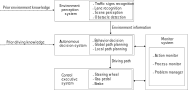
\includegraphics[width=11cm,height=18cm,keepaspectratio]{chapters/Chapitre_2/Figures/AV_Architecture.png}
        %\vspace{-2.3mm}
        \caption{AV's architecture \cite{ni2020survey}}
        \label{fig:AV_Architecture}
        \end{figure}


The environment \textbf{perception} system utilizes the prior knowledge of the environment to establish an environmental model including obstacles, road structures, and traffic signs through obtaining surrounding environmental information. The main function of the environment perception system is to realize functions like lane detection, traffic signal detection, and obstacles detection, by using some hardware devices such as cameras, LiDARs and radars.  

The main function of the autonomous \textbf{decision} system is to make some decisions for the self-driving car, including obstacle avoidance, path planning, navigation, and so on. For example, in the path planning, the autonomous decision system plans a global path according to the current localization and the target location firstly, then reasonably plans a local path for the self-driving car by combining the global path and the local environment information provided by the environment perception system.   

The \textbf{control} execution system's function is to generate the commands needed to meet the objectives given by the decision system, such as braking, steering, and accelerating to guarantee the speed control and path-following control. 

The \textbf{monitor} system is responsible to check whether the car is making actual progress towards its goal and reacts with recovery actions when meeting problems like unexpected obstacles and  faults.

\subsection{Multi-Vehicle System} \label{sec: MVS_control_Architecture}
Most of the current industrial developments and applied researches in the area of autonomous vehicles concern the methods and tools to enable \textit{individual} autonomous vehicles to hit the road safely. However, it is getting increasingly recognized that, to get full advantage from the autonomous vehicle technology, a number of situations will compulsory require \textit{coordinating} the relative activities and movements of the vehicles \cite{10.1007/978-3-030-03424-5_6} \cite{6949576}.


Consequently, a natural extension of an \textit{individual} autonomous vehicle is to deal with MVS, with the help of \textit{coordination}. MVS, which have shown immense promise as a component of future transportation systems \cite{chai2017connected} \cite{C-Roads} \cite{sjoberg2017cooperative}, will be further discussed in the rest of the section. Not that the proposed MVS makes the assumption that connection is always available, either locally or globally. MVS provide appealing benefits in terms of operating in constrained environment, resolving problems concurrently, considerably reducing accidents and related costs.   

Around the globe, car manufacturers and research institutes are starting to move away from the vision of building autonomous vehicles that are completely autarkic from their surroundings and towards including communication into their cars. Recent surveys cover benefits of such communication for autonomous driving \cite{wang2018networking} \cite{5G}. Vehicle connectivity is a new technology that enables Vehicle-to-Infrastructure (V2I), Vehicle-to-Vehicle (V2V) and Vehicle-to-Everything (V2X) communication \cite{blum2004threat} \cite{machardy2018v2x}. Vehicles equipped with interactive Advanced Driver Assistance Systems (ADAS) and Cooperative Intelligent Transportation Systems are typically considered to be connected \cite{uhlemann2015introducing}. Car connectivity may give both the regular vehicle and the autonomous vehicle new information and services. MVS are capable of receiving information from the V2X outside the field of vision and negotiating with other road users. Thus, MVS may outperform the \textit{individual} intelligent vehicle not only in terms of safety and performance, but also in terms of traffic throughput and fuel efficiency via global route planning and cooperative driving \cite{eskandarian2019research}.

The connected ecosystem provided by the V2X paradigm linked to the autonomous vehicle technology permits to unlock new innovative mobility solutions just to mention a few: car sharing \cite{goodrich2008human}, where fleets of autonomous vehicles will be available to serve our urban mobility needs; personalized public transport and ride sharing  \cite{OnRecommending}\cite{stiglic2018enhancing}, where autonomous vehicles and buses can dynamically gather people based on their actual required routes; smart and more effective parking approaches \cite{lin2017survey}, in that autonomous vehicles can search for parking slots based on criterion different from the very soon and very close, one that humans usually adopt, and exploiting additional information that they might have. 

It is difficult to test these innovative mobility solutions on public roads, and there is a lack of experimental validation in real-world conditions \cite{guanetti2018control}. Therefore, several programs based on MVS have been established by governments and national organizations. The following section gives an overview of MVS projects around the world. 

\subsection{Overview of MVS projects around the world}\label{sec:MVS_Projects_Overview}


In this section it is proposed to delve into the projects related to the MVS. These projects epitomize the technological advancements and innovations dedicated to enhancing the capabilities of MVS when navigating in on-road dynamic environments such as highways. 

\subsubsection{PATH} \label{PathProject}
Partners for Advanced Transportation Technology (PATH) 
\cite{PathProject1} (cf. Figure \ref{fig:path_project}) is a research and development program of the University of California, Berkeley, has been a leader in Intelligent Transportation Systems research since its founding in 1986. In collaboration with the California Department of Transportation (Caltrans), administered by the university’s Institute of Transportation Studies, PATH is a multi-disciplinary program with staff, faculty, and students from universities worldwide and cooperative projects with private industry, state and local agencies, and nonprofit institutions.

The PATH research on automated platoons was initially motivated by the need to produce a significant increase in the capacity of a highway lane, so that increases in travel demand could be accommodated with a minimum of new infrastructure construction. The PATH studies of highway capacity showed that it could be possible to increase lane capacity by factor of two to three over today's capacity if the vehicles were driven in platoons of up to ten cars \cite{michael1998capacity}. The gaps between platoons would be long enough to ensure that even in the worst crash hazard condition, with maximum deceleration, a following platoon would be able to stop without hitting the last vehicle of the forward platoon. An extensive modeling and simulation study of crash safety and capacity showed the advantages of the platoon mode over individual automated vehicle \cite{carbaugh1998safety}. The PATH studies have been based on the assumption that all vehicles would be automated, including the first vehicle on the platoon. 

PATH first tested the longitudinal control of a four cars platoon at highway speeds in 1994, and then a demo based on eight cars platoon was developed for the National Automated Highway System Consortium (NAHSC) in 1997. The latter included a large set of maneuvers; car following, lane change, joining and leaving platoon to cite a few, all under completely automatic control. 

More recently, the PATH platooning research has focused on heavy trucks, mainly because of the potential of energy saving associated with aerodynamic drag reductions. Operating tractor-trailer trucks in close-formation automated platoons of three trucks could enable a capacity of about 1500 trucks per lane per hour \cite{bergenhem2012overview}. The PATH experiments on truck platoons have shown the technical feasibility of driving two trucks at a gap of 3m and three trucks at a gap of 4m between trucks. These experiments have also shown direct fuel consumption savings in the range of 5\% for the lead truck and 10\% to 15\% for the following trucks. 

\begin{figure}[!h]
        \centering 
        \includegraphics[width=8cm,height=18cm,keepaspectratio]{chapters/Chapitre_2/Figures/Path_project.png}
     %   \vspace{-2.3mm}
        \caption{Highway cooperative navigation part of the PATH project \cite{PathReport}}
        \label{fig:path_project}
        \end{figure}





\subsubsection{Demo 2000}
A demonstration on the cooperative driving with five automated vehicles was conducted in November 2000 part of the Demo 2000 cooperative driving project to show the feasibility and potential of the technologies \cite{tsugawa2000introduction}. The cooperative driving in Figure \ref{fig:Demo_2000}, aiming at the increase in the safety and throughput of road traffic, here means that automated vehicles are driven in a flexible platoon with a short inter-vehicle distance over a couple of lanes. The vehicles of the demonstration are equipped with RTK-GPS \cite{tsugawa2001cooperative} for vehicle localization, a laser radar detection of an obstacle or a preceding vehicle, the inter-vehicle communication unit, and the onboard display for the passenger to locate the neighboring vehicles. The localization data are employed for the lateral and the longitudinal control of the automated vehicle with the precise map of the demonstration site. The data on the localization and speed  of each vehicle in the platoon and the location of the obstacles are transmitted at every 100 milliseconds over the inter-vehicle communication. The protocol, nicknamed as DOLPHIN (Dedicated Omni-purpose inter-vehicle communication Linkage  Protocol for Highway automatIoN) after the ecology of the dolphins, is designed for the dedicated use in the demonstration. The five automated vehicles drove at 40 - 60 km/h on a test track according to the demonstration scenario including stop and go, platooning, lane changing, merging, and obstacle detection and avoidance \cite{tsugawa2001demo}.   


\begin{figure}[!h]
        \centering 
        \includegraphics[width=8cm,height=18cm,keepaspectratio]{chapters/Chapitre_2/Figures/DEMO2000.PNG}
       % \vspace{-2.3mm}
        \caption{Platoon navigation under the DEMO 2000 project \cite{fujioka2002its}}
        \label{fig:Demo_2000}
        \end{figure}


\subsubsection{Scania platooning}
Fuel is one of the largest cost for a fleet owner \cite{bergenhem2012overview} \cite{aarts2016european}. Therefore, systems that reduce fuel consumption are high financial interest for fleet owners. Reducing the fuel consumption also reduces the environmental effect of the transport. Scania's main interest in the platooning is hence focused on heavy-duty  goods vehicle platooning on highways (cf. Figure \ref{fig:Scania_platooning}) with a highlight on fuel consumption minimization \cite{alam2015heavy}. 


Distributed control of a heavy-duty vehicle platoon is a collaboration between Scania and the Royal Institute of Technology, and is partly funded by the Swedish government. The main focus of the project is how a single vehicle operating in a platoon should be efficiently controlled without jeopardizing safety. Longitudinal movement is autonomously controlled while lateral movement is manual. The control architecture has been developed based on a distributed control, meaning that each vehicle is responsible for its own control, based on information from onboard sensors (e.g., radar, cameras) along with, information exchange between the vehicles in the platoon via V2V communication. 

% (b) iQFleet, is a collaboration between the KTH, the Swedish National Road and Transport Research Institute, The Swedish Transport Administration and is partly funded by the Swedish government. The project covers several research topics where platooning is one. Platooning research is focused on how platoons should be controlled w.r.t. other road users, road topology, instracture, etc. The goal is to develop strategies and architecture that support driving and routing a number of platoons in an optimal way w.r.t. the road conditions. iQFleet 

It also includes real road tests of platooning. The trial takes place between two Swedish cities and it aimed to: 
\begin{itemize}
    \item Investigate the fuel saving potential in real traffic conditions, 
    \item Evaluate the driver acceptance, 
    \item Analyze interactions between the platoon and the surrounding traffic. 
\end{itemize}

\begin{figure}[!h]
        \centering 
        \includegraphics[width=8cm,height=18cm,keepaspectratio]{chapters/Chapitre_2/Figures/Scania_platooning.jpg}
       % \vspace{-2.3mm}
        \caption{Scania platooning  [image courtesy of Scania]}
        \label{fig:Scania_platooning}
        \end{figure}
%For validity of the trials, the trucks were driven by professional trucks drivers. In the first phase, the platoon uses existing Adaptive Cruise Control based on radar information. The gap between the trucks was 2-3s, which corresponds to 40-60m. In the second phase, V2V communication was introduced, what shortened inter-trucks distance. 


\subsubsection{Energy ITS}
A national Intelligent Transportation System (ITS) project by the Japanese Ministry of Economy, Trade and Industry, started in 2008, aims at energy saving and global warming prevention with ITS technologies \cite{TSUGAWA201341}\cite{OHTA2023100187}. The latter has two themes: an automated truck platoon and an evaluation method of effectiveness of ITS on energy saving. Another motivation for the project is mitigating the lack of skilled drivers. On a test vehicle, a platoon of three completely automated heavy trucks and one fully automated light truck traveled at 80 kilometers per hour with a distance of up to 10 meters \cite{tsugawa2014results}. The lateral control is based on the lane marker detection by the computer vision, and the longitudinal control is based on the gap measurement by the lidar, radar and the V2V communication (cf. Figure \ref{fig:Energy_ITS}). According to the trial, platooning of 10m gap at 80 km/h can reduce energy by about 15\%  (measurement) by the aerodynamic drag reduction, and $CO_{2}$ by 2.1 \% (simulation) \cite{tsugawa2011automated}. Additionally, this research included testing on four heavy-duty trucks equipped with Cooperative Adaptive Cruise Control (CACC) \cite{tsugawa2014results}. 



\begin{figure}[!h]
        \centering 
        \includegraphics[width=9cm,height=18cm,keepaspectratio]{chapters/Chapitre_2/Figures/ITS.png}
      %  \vspace{-2.3mm}
        \caption{Configuration of the automated truck part of the Energy ITS project \cite{tsugawa2014results}}
        \label{fig:Energy_ITS}
        \end{figure}







\subsubsection{SARTRE}
The SARTRE program (SAfe Road TRains for the Environment) \cite{bergenhem2010challenges}\cite{chan2016sartre} is an European Commission Co-Funded project that seeks to support a change in transport utilization. The project vision is to develop and integrate solutions that allow vehicles to drive in platoons on public roads without modification of the infrastructure. SARTRE train defines a platoon as a collection of vehicles led by manually driven heavy-duty vehicles. The vehicles behind follow the lead vehicle automatically; both laterally and longitudinally (cf. Figure \ref{fig:SARTRE}). Vehicles may join or leave the platoon dynamically (e.g., leave on arrival at the destination). SARTRE expected advantages of platooning include a reduction in fuel consumption, increased safety, traffic efficiency, increased driver convenience and comfort \cite{chan2012cooperative}\cite{2011-36-0060}.



\begin{figure}[!h]
        \centering 
        \includegraphics[width=9cm,height=18cm,keepaspectratio]{chapters/Chapitre_2/Figures/SARTRE.jpg}
        \caption{SARTRE project demonstration [image courtesy of the Volvo car corporation]}
        \label{fig:SARTRE}
        \end{figure}



\subsubsection{Grand Cooperative Driving Challenge} \label{sec:GCDC}
Low cost and reliable communication systems have recently renewed the interest in MVS. In the 2011 Grand Cooperative Driving Challenge (GCDC) (cf. Figure \ref{fig:GCDC2011}) \cite{bergenhem2010challenges}\cite{ploeg2012introduction}\cite{maartensson2012development}\cite{guvencc2012cooperative}, nine international teams joined the challenge with the purpose of supporting and accelerating the introduction of MVS in everyday traffic through a driving challenge. Two scenarios, one urban and one highway, were performed. The urban scenario featured two platoons standing one after the other with a certain distance. The task was to let the rear platoon join the foremost platoon with minimum disturbances. The highway scenario focused on the platooning performance, where a lead vehicle from the organizers guided the participating vehicles in maneuvers. 

For both scenarios, evaluation criteria were based on total platoon length, platoon length variations, vehicle gap length, and string stability. The vehicles incorporated automated longitudinal control, whereas the drivers manually operated the lateral steering. The 2011 GCDC focused on forming platoons, while basic platoon operations such joining from rear on a single lane were performed, and complicated operations such as platoon merging from two parallel lanes were out of reach. The winner of the 2011 GCDC winner was Team AnnieWay; a group of researchers hosted at Karlsruhe Institute of Technology (Karlsruhe, Germany) \cite{geiger2012team}. 

Many challenges surfaced during the 2011 GCDC, ranging from different interpretation of standards (e.g., time, position) to issues with radar reflections. One of the main challenges that occurred was related to wireless communication, where all participants should intercept the transmitted information in the same way. 

While 2011 GCDC focused on basic platooning such as forming and maintaining a platoon, the 2016 GCDC \cite{ploeg2017cooperative} aimed to demonstrate how cooperative automated vehicles can perform complicated platooning operations with close to reality traffic scenarios (cf. Figure \ref{fig:GCDC2016}). In addition to the Heudiasyc team, nine other teams were part of the 2nd GCDC edition and were challenged through two typical environments; highway and urban intersection \cite{englund2016grand}. 

Advanced platoon operation was investigated in the 2016 GCDC. The cooperative platoon merge scenario involved two platoons driving on a highway on different lanes that must merge into one platoon. A competition zone was defined within which the vehicles' operations were judged. Highway scenario included common events on road traffic (e.g., road works, lane closure, traffic merge). 

Intersections are one of the most critical and challenging traffic environments that are attracting significant works \cite{chen2015cooperative}. In order to showcase MVS abilities, a cooperative urban non-controlled intersection was considered. To be more realistic, the latter involved non-communicating vehicles. In addition, a third scenario was considered, including an emergency vehicle that required passage in a congested traffic situation. Team Halmstad from the Halmstad University (Halmstad, Sweden) won the challenge \cite{aramrattana2018team}. 



In Table \ref{tab:Summary_project} a summary of the above discussed project is given. 


\begin{figure}[ht]
\begin{minipage}[b]{0.45\linewidth}
\centering
\includegraphics[width=\textwidth]{chapters/Chapitre_2/Figures/GCDC2011.png}
\caption{GCDC 2011 [image courtesy of IEEE]}
\label{fig:GCDC2011}
\end{minipage}
\hspace{0.5cm}
\begin{minipage}[b]{0.45\linewidth}
\centering
\includegraphics[width=1.05\textwidth]{chapters/Chapitre_2/Figures/GCDC2016.jpeg}
\caption{GCDC 2016 [image courtesy of IEEE]}
\label{fig:GCDC2016}
\end{minipage}
\end{figure}




% %%%%%%%%%%%%%
% \newenvironment{changemargin}[2]{%
% \begin{list}{}{%
% \setlength{\topsep}{-4pt}%
% \setlength{\leftmargin}{#1}%
% %\setlength{\rightmargin}{#2}%
% \setlength{\listparindent}{\parindent}%
% \setlength{\itemindent}{\parindent}%
% \setlength{\parsep}{\parskip}%
% }%
% \item[]}{\end{list}}
% %%%%%%%%%%%%



\newpage
\thispagestyle{empty}

\begin{landscape}
  \begin{adjustwidth}{-0.20\textwidth}{-0.20\textwidth}

\begin{table}[]
\resizebox{21cm}{!}{
\centering

\begin{tabular}{|c|c|c|c|c|c|l|}
\hline
                                                                         & Vehicle type                                                          & Control                                                             & Infrastructure requirement                                                       & Traffic integration                                                         & Sensors                                                       & \multicolumn{1}{c|}{Goals}                                                                                                                             \\ \hline
PATH (1986 - 1997)                                                       & \begin{tabular}[c]{@{}c@{}}Cars or heady \\ duty trucks\end{tabular}  & \begin{tabular}[c]{@{}c@{}}Longitudinal \\ and lateral\end{tabular} & \begin{tabular}[c]{@{}c@{}}Reference markers\\  in road surface\end{tabular} & \begin{tabular}[c]{@{}c@{}}Dedicated lane \\ (highway focused)\end{tabular} & Mixed                                                         & \begin{tabular}[c]{@{}l@{}}- Energy savings \\ - Increase traffic throughput\end{tabular}                                                                  \\ \hline
Demo 2000 (2000)                                                         & Cars                                                                  & \begin{tabular}[c]{@{}c@{}}Longitudinal \\ and lateral\end{tabular} & None                                                                         & Mixed                                                                       & Mixed                                                         & \begin{tabular}[c]{@{}l@{}}- Demonstrate platooning efficiency \\- Build a dolphin inspired \\ communication protocol\end{tabular}                        \\ \hline
\begin{tabular}[c]{@{}c@{}}Scania platooning \\ (2001- now)\end{tabular} & heavy-duty trucks                                                     & Longitudinal                                                        & None                                                                         & \begin{tabular}[c]{@{}c@{}}Mixed \\ (highway focused)\end{tabular}          & Mixed                                                         & \begin{tabular}[c]{@{}l@{}}- Fuel savings\\ - Demonstrate complex \\ maneuvers using platooning\end{tabular}                                              \\ \hline
\begin{tabular}[c]{@{}c@{}}Energy ITS \\ (2008 - 2012)\end{tabular}      & heavy-duty trucks                                                     & \begin{tabular}[c]{@{}c@{}}Longitudinal \\ and lateral\end{tabular} & Lane markers                                                                 & Dedicated lane                                                              & Mixed                                                         & \begin{tabular}[c]{@{}l@{}}- Mitigate lack of skilled drivers \\- Energy saving\end{tabular}                                                              \\ \hline
\begin{tabular}[c]{@{}c@{}}SARTRE \\ (2009 - 2012)\end{tabular}          & \begin{tabular}[c]{@{}c@{}}Cars and heavy \\ duty trucks\end{tabular} & \begin{tabular}[c]{@{}c@{}}Longitudinal \\ and lateral\end{tabular} & None                                                                         & \begin{tabular}[c]{@{}c@{}}Mixed \\ (highway focused)\end{tabular}          & \begin{tabular}[c]{@{}c@{}}Production \\ sensors\end{tabular} & \begin{tabular}[c]{@{}l@{}}- Increase safety and passengers' \\ comfort \\ - Reduce road congestion, \\ along with energy saving\end{tabular}                 \\ \hline
1st GCDC (2011)                                                          & Cars mainly                                                           & Longitudinal                                                        & None                                                                         & \begin{tabular}[c]{@{}c@{}}Mixed \\ (highway focused)\end{tabular}          & Mixed                                                         &\begin{tabular}[c]{@{}l@{}}- Accelerate MVS deployment \\ - Demonstrate platooning  feasibility\end{tabular}\\ \hline
2nd GCDC (2016)                                                          & Cars                                                                  & \begin{tabular}[c]{@{}c@{}}Longitudinal \\ and lateral\end{tabular} & None                                                                         & Mixed                                                                       & Mixed                                                         & \begin{tabular}[c]{@{}l@{}}- Outperform complex platooning \\maneuvers \\ - Demonstrate cooperative \\ intersection crossing feasibility\end{tabular} \\ \hline
\end{tabular}
}
\caption{Summary of the major project involving MVS}
\label{tab:Summary_project}
\end{table}
\end{adjustwidth}

\end{landscape}
\newpage





\section{Cooperative navigation for MVS: scenarios overview} \label{sec: CooperativeNavigation-Scenarios Overview}
The challenge of \textbf{coordinating} the actions and interactions of MVS within on-road environments in a vast multifaceted one. This challenge encompasses an array of highly diverse scenarios, ranging from scenarios involving cooperative merging on highway on ramps, as well as, employing tools such as Cooperative Adaptive Cruise Control (CACC) for tasks like platooning. To urban settings involving cooperative navigation through signalized and non-signalized intersections. Despite this apparent diversity, these varied scenarios can be effectively unified and conceptualized within a coherent framework (cf. Figure \ref{fig:CAV_applications}). 



With \textbf{coordination} we refer to the decision-making and planning (involving vehicles themselves and possibly some additional infrastructure process) aimed at orchestrating vehicle' actions as to achieve a goal which cannot be achieved (or not optimally) by each vehicle in isolation. The coordination goal may belong either to an individual vehicle (e.g., intersection crossing), or to a group of vehicles (e.g., platoon navigation), or even the traffic system as a whole (e.g., improving the city traffic flow) (cf. Figure \ref{fig:CAV_applications}).  

In the following section, it is proposed an overview of the topics related to the problem of coordinating the motion of MVS from the scenario perspective. 


\begin{figure}[!h]
        \centering 
        \includegraphics[width=11cm,height=18cm,keepaspectratio]{chapters/Chapitre_2/Figures/Schema_cooperative.png}
        %\vspace{-2.3mm}
        \caption{MVS applications: an overview}
        \label{fig:CAV_applications}
                \vspace{-5mm}
        \end{figure}
\subsection{Cooperative navigation in urban environment}

% il faut citer le CGDC 2016 avec la gestion d'intersection en mode cooperatif et renvoyer vers le projet que je detail un peu plus haut 
% introduction 
In urban core areas, MVS navigation becomes highly difficult under a variety of urban situations involving numerous road users. Several MVS applications have been explored to benefit safety, mobility and the environment with connected vehicles \cite{karmanska2021benefits}\cite{CAVBenefits}\cite{congestion2}. Among them, MVS cooperation technology for intersection or roundabout applications attract representative and significant efforts. More precisely, research on MVS cooperative driving is conducted at both signalized and unsignalized intersection/roundabout. 


% definition de la coordination 
Intersection crossing (cf. Figure \ref{fig:intersection}) and roundabout (cf. Figure \ref{fig:roundabout}) navigation in urban areas is the problem of coordinating vehicles' motions while concurrently navigating through the intersection/roundabout. According to \cite{mariani2021coordination}, the problem of intersection/roundabout is a competitive resource-oriented problem, where the vehicles are self-interested agents willing to obtain the right-of-way as soon as possible across the shared resource represented by the intersection/roundabout.  


        \begin{figure}[!h]
        \centering 
        \includegraphics[width=10cm,height=18cm,keepaspectratio]{chapters/Chapitre_2/Figures/Intersection.PNG}
        %\vspace{-2.3mm}
        \caption{Cooperative intersection crossing}
        \label{fig:intersection}
              %  \vspace{-5mm}
        \end{figure}

        \begin{figure}[!h]
        \centering 
        \includegraphics[width=10cm,height=18cm,keepaspectratio]{chapters/Chapitre_2/Figures/Driving School.PNG}
        %\vspace{-2.3mm}
        \caption{Cooperative roundabout crossing}
        \label{fig:roundabout}
               % \vspace{-5mm}
        \end{figure}

% le problème c'est quoi
Today, intersections management is realized either by a central controller, the traffic light, or by imposing to vehicles (i.e., the drivers) pre-defined coordination rules to be obeyed (e.g., stop at sign or give the right-of-way to vehicles coming from the right), as well as for roundabout \cite{7562449}. This put the responsibility for safety fully in charge of humans, and not promote efficiency. 

% les solutions possibles mais qui ne sont pas possible à la fois
To tackle the problem of intersection/roundabout navigation, it is possible (i) to act on the supply side, increasing the number of roads or lanes in a network, (ii) to reduce the demand, restricting the access to urban areas at specific hours or to specific vehicles, or (iii) to improve the efficiency of the existing network, by means of a widespread use of MVS.

% la solution avec les CAVs et la communication 
In fact, with the help of V2V communication and/or V2I communication, it is possible to conceive a variety of innovative solutions, safer and more efficient. Roughly, V2I communication is often preferred at signalized intersections in order to get Signal Phase and Time (SPaT) information and prevent unnecessary speed changes or complete stops \cite{Eco-Approach}.

 Within an intelligent transportation system, V2V and V2I communications are often used at intersection/roundabout  \cite{guanetti2018control}\cite{wang2019survey}, eventually making traffic light and stop signs obsolete. With the help of V2V and/or V2I communication, the possibility of sharing future intentions among vehicles is feasible, helping to prevent conflicting trajectories. Thus, following the planning and scheduling algorithm, MVS can be assigned specific sequences to cross the intersection/roundabout. Alongside, communication offers opportunity to optimize the passing order, also known as passing sequence, among the vehicles within a certain communication range, this means that the navigation task through the intersection/roundabout can be seen as a global task related to the participating vehicles, where each vehicle has its own passing order provided by a multi-criterion function. This cooperative behavior permits to translate the problem of intersection/roundabout from a competitive resource-oriented task to a cooperative altruistic-task oriented, where the global aim tackles the traffic throughput, idling time at intersection/roundabout and energy efficiency, in addition to risk metrics.

In fact, the research work related to MVS navigation coupled with V2V/V2I communication in intersection/roundabout has gained considerable attention during the last decades. Comprehensive surveys about this problem are analyzed in \cite{chen2015cooperative}\cite{elliott2019recent}\cite{guo2019urban}\cite{namazi2019intelligent}\cite{rasheed2013fleet}. 

%\textcolor{blue}{ajouter une figure avec plusieurs intersection et des roundpoint un peu comme dans la these de zhang en ajoutant une signalized intersection/roundabout et une unsignalized intersection/roundabout}


%The authors in \textcolor{red}{ajouter la reference 513 de la these de zhang} propose an Eco-CACC algorithm that computes the most fuel-efficient vehicle trajectory through a signalized intersection by guarantying that the vehicle arrives at the intersection stop bar as soon as the last connected vehicle in the queue is dischargedµ. The work in \textcolor{red}{ajouter la reference 540 de la these de zhang} considers a real-time 









\subsection{Cooperative navigation in highway environment}
Among the maneuvers performed by the vehicle on a highway environment one can cite on/off-ramp merging \cite{7562449}\cite{zhu2022merging}, platoon navigation \cite{kavathekar2011vehicle}, lane change \cite{moridpour2010lane}. Some of these maneuvers can be challenging since they involve numerous road users performing at high maneuvers \cite{dey2015review}. 
 
% pourquoi intégrer les ITS dans les highways, les CAVs avec la communication et les avantages de cette intégration.
With the significant developments achieved during the last decade with the help of intelligent transportation systems, addressing mobility issues on highway become possible. The integration of MVS on highway environment appears to be the next ITS move and the natural extension to the aforementioned mobility technology. Mainly because, in one hand, under the MVS paradigm, collaborative navigation on a highway addresses the problem of coordinating the vehicle's maneuvers, so they travel together without causing any collision risk \cite{bayat2017environmental}\cite{faisal2019understanding}\cite{montanaro2019towards}. In the other hand, connectivity integrated in MVS, make them capable to not only drive by themselves with on-board sensors, but also to communicate with each other with the help of the V2V communication \cite{hakak2022autonomous}\cite{balador2022survey}. Consequently, it improves road safety where future actions can be well anticipated where a better understanding of the navigation scene can be built. Beside the safety benefits, MVS technology associated with communication permits to increase traffic throughput by reducing safety distance between MVS, and to improve energy efficiency by avoiding unnecessary speed changes \cite{bagloee2016autonomous}. 

%Based on the impact of CAVs technology on highway, it has garnered considerable attention during the last decade. Moreover, it is seen in the literature as an auspicious technology not only to tackle traffic throughput on highway, but also to overcome the safety and the mobility issues related to on-off ramp merging on highways.  


Over the past decade, the impact of MVS technology on highways has captured significant attention. This innovative technology is regarded in the literature as promising, not only for addressing traffic congestion on highways but also for enhancing safety and mobility by addressing the challenges associated with on/off ramp merging. An overview addressing the utilization of the MVS technology in the context of highway navigation in platoon is provided in Section \ref{sec:platooning_navigation}. Section \ref{sec:on-ramp merging} specifies MVS utilization in the context of on-ramp merging on highway. 

\subsubsection{Cooperative platooning navigation on highway}\label{sec:platooning_navigation}
% introduction des applications comme le platooning 
On the highway, human driven vehicles have a natural tendency to follow one another closely and operate within a phenomenon known as longitudinal formation or platooning (cf. Figure \ref{fig:Merging}). For a human-operated vehicle, a platoon-based formation can be considered as basic behavior, and it can be easily distinguished in everyday life. However, for MVS, they must stay in the same lane and follow nearby vehicles by maintaining safe distance and velocity, to form the desired longitudinal shape. The aim of the platoon formation control is to confirm that all the vehicles in a platoon move at the same speed while maintaining the desired geometry, which is stated by a desired inter-vehicle spacing strategy \cite{hafner_survey_2022}. Therefore, for MVS, platoon formation requires specific algorithms, controllers and strategies.


\begin{figure}[!h]
        \centering 
        \includegraphics[width=10cm,height=18cm,keepaspectratio]{chapters/Chapitre_2/Figures/merging.PNG}
      %  \vspace{-2.3mm}
        \caption{Cooperative merging on highway}
        \label{fig:Merging}
             %   \vspace{-5mm}
        \end{figure}

It was under the PATH (cf. Section \ref{PathProject}) research project that the current CACC implementation in production vehicles was mainly developed as the extension of the commercially available ACC system \cite{6588305} (cf. Figure \ref{fig:CACC}). Therefore, most CACC vehicles are also equipped with sensors installed on ACC vehicles, such as odometers, radar and/or LiDAR, along with communication. Given the fact that the communication bandwidth might become insufficient when the number of MVS increases in a CACC system, short ranged wireless technologies are more accepted for V2V communication \cite{Grilli}. By sharing vehicle information such as acceleration, speed and position, MVS in the communication range can cooperate to increase highway capacity \cite{ren2008distributed}.



%Communication topology is a cornerstone in the CACC technology \cite{8569947}. The information flow topology defines the way CAV obtains information from other CAV in a CACC system. %Some typical types of information flow topologies include predecessor-following, predecessor-leader following, two predecessor-following, two predecessor-leader following and bidirectional types . 







\begin{figure}[!h]
        \centering 
        \includegraphics[width=10cm,height=18cm,keepaspectratio]{chapters/Chapitre_2/Figures/CACC.PNG}
      %  \vspace{-2.3mm}
        \caption{Cooperative adaptive cruise control: platooning navigation}
        \label{fig:CACC}
              %  \vspace{-5mm}
        \end{figure}

%In this section collaborative navigation of MVS in highway using platooning will be discussed through its impact on highway throughput, and on energy efficiency. The cooperative Adaptive Cruise Control (CACC) is presented as a tool to perform cooperative navigation on highway. 






%The latter is based on the extension of Adaptive Cruise Control (ACC) with cooperative maneuvers by CAVs. \textcolor{red}{ajouter la reference A review on Cooperative Adaptive Cruise Control systems: Architectures, controls and applications}. 

%Cooperative Adaptive Cruise Control (CACC) is one of the most promising technologies for CAVs platooning navigation on highway. At the heart of the concept of CACC is the merging of Adaptive Cruise Control (ACC), a subset of the broader class of automated longitudinal speed control systems, with a cooperative module enabled with the V2V/V2I \textcolor{red}{ajouter la bonne reference, voir le rapport bibio}. 



%The development made in communication field permit to communicate information between the CAVs using the V2V communication, and between the CAVs and the infrastructure with the help of the V2I communication. 








  
 
 In CACC systems, MVS share their own data with other MVS in the network by V2V communications, which is realized in a distributed manner without central management \cite{1402433}.
 
 CACC takes advantages of V2V communications to allow MVS to form platoons and be driven at harmonized speeds with short-time headway between them.  MVS in a certain communication range can cooperate with others to obtain the following benefits: (i) driving safety is increased since actuation time is shortened compared to manually driven, and downstream traffic can be broadcasted to following vehicles in advance; (ii) roadway capacity is increased due to the reduction of time/distance headway between vehicles; (iii) energy consumption and pollutant emissions are reduced due to the reduction of unnecessary velocity changes and aerodynamic drag on following vehicles \cite{massar2021impacts}. 

\subsubsection{Cooperative on-ramp merging on highway}\label{sec:on-ramp merging}


Traffic merging at highway on-ramps (cf. Figure \ref{fig:OnRamp}) is a major conflict that generates safety and mobility concerns. The difficulty arises for the AV along the on-ramp where it has to discern whether to accelerate or decelerate to enter the main line safely and may not have a clear line of sight. Meanwhile, the mainline highway users may have to modify their speeds to permit the entrance of merging AV, thus affecting traffic flow which may result in road congestion. To address these issues, cooperative MVS have was studied and applied to the highway on-ramp merge case, where different control algorithms have been proposed and implemented to allow MVS to merge with each other in a cooperative manner. Existing related works have been reviewed in \cite{7562449}. 

 
 
 
 \begin{figure}[!h]
        \centering 
        \includegraphics[width=10cm,height=18cm,keepaspectratio]{chapters/Chapitre_2/Figures/OnRamp.png}
        %\vspace{-2.3mm}
        \caption{Cooperative on-ramp merging on highway}
        \label{fig:OnRamp}
              %  \vspace{-5mm}
        \end{figure}
 
 

 
 
 
 
 
 
 
 
 
 
 
 
 
 
 
 
 








\section{Conclusion}




In this chapter, a comparison between single autonomous vehicle systems and multi-vehicle systems is explored. Since MVS comprises several individual AVs in a cooperative manner, this chapter provides a summary of the mechanisms employed by the AVs within their control architecture, paving the pay for the presentation of the MVS paradigm. An extensive overview of prominent projects involving MVS is presented. Additionally, the chapter delves into contexts where MVS finds utility in dynamic and challenging on-road environments. It examines relevant works related to both urban cooperative navigation and highway platooning navigation, in addition to the on-ramp merging on highway. Finally, the chapter highlights the significant advantages of utilizing MVS in various scenarios, with a particular focus emphasis on highway context. 
 

  \chapter{Cooperative Motion Planning and Decision-Making for MVS: Architecture Overview} \label{sec: CooperativeNavigation_GlobalOverview} \label{chap:chapter2}




\begin{abstract}
This chapter is devoted to providing a comprehensive overview of MVS control architecture. It delves into an exploration of pertinent literature, examining the various applications of MVS across different domains. The chapter sheds light on the paradigms employed in constructing MVS control architecture. Furthermore, it offers a detailed literature review of MVS applications within complex and dynamic environments.
    
\end{abstract}


\textbf{Contents}
\vspace{0.15cm}
\hline
\hspace{2cm}
\localtableofcontents
\hspace{2cm}
\hline











\section{Introduction}
% TODO
%% Give an introduction about the importance of AV in acadimia and link it to Zhing's diagram
%% Introduce the idea of acadimia being interessted about the MVS and give one old reference about MVS to prove that MVS are pretty old a topîc of interest in acadimia 
%% donner un cahier des charges de sur quoi le MVS doit respecter un peu comme le fait Zhang (page 39)
%% Need to introduce the idea of several types of architecture (centralized/ distributed/ hybride) 
%%  ajouter une section sur les architecture multi-controller/ behaviors pour introduire le fait que j'ai plusieurs behaviors (voir livre lounis page 17 et la thèse de Vilca surement) 
%% Need to introduce the idea that we do have a variaty of methods that rely on several levels (decision, communication, control) to precise our scoop which is (decision and control) not communication. 


In the recent years, the automotive research and industry has undergone a profound transformation, driven by rapid advancements in technology and a growing emphasis on safety, sustainability and efficiency. At the forefront of this evolution, one concept is pointed to revolutionize the way we think about transportation: Multi-Vehicle System (MVS). These cutting edge technologies represent the fusion of several years of development of the automated vehicles, connectivity and automotive engineering, promising to reshape not only the way we move and travel but also our urban environment and our roads. 




The primary objective of this chapter is to provide an extensive overview of the MVS control architecture, along with the examination of the relevant literature concerning the utilization of MVS across diverse applications. Section \ref{sec:control_architecture_for_MVS} outlines the various modules and process integrated in the MVS control architecture. In Section \ref{sec:MVS_control_Architecture}, an insight into the paradigms employed in constructing the MVS control architecture is presented. Formation control stands as an important aspect of the MVS paradigm, and thus, in Section \ref{sec: formation_control_theory}, a comprehensive review of various formation control approaches is conducted. Lastly, Section \ref{sec:review_MVS_application} provides a literature review highlighting MVS applications within complex environments.  


% je peux continuer cette section avec l'explication de ce qu'on va trouver dans les sections plus bas à savoir expliquer les architecture, et les méthodes utilisées avec le classement --- un truc en mode in this section .... blablabla 

\section{Control architecture for MVS} \label{sec:control_architecture_for_MVS}
% enfaite deja là on commence a parler de l'architecture du véhicule. 
Automated Vehicles (AVs), known as self-driving cars or autonomous vehicles, have captured the imagination of the public, scientists and industry alike during three decades. These vehicles leverage sophisticated sensors, complex decision-making processes and real-time data analysis to navigate the roads with minimal to absence of human intervention. The promise of improved safety, enhanced energy management, reduced congestion, and increased accessibility has fueled intense research and development. One consensus started to emerge between the contributors to the AVs developments; to take full advantages of the AV technology, AVs must collaborate with the road users.

On the other hand, MVS takes the concept of driving automation to the next level by introducing a collaboration level between vehicles, infrastructures, and even pedestrians. This inter-connectivity has the potential to induce numerous benefits such as enhancing safety, more efficient energy consumption and real-time traffic optimization (cf. Section \ref{sec: CooperativeNavigation-Scenarios Overview}).  

The autonomous management of a fundamental MVS essentially encompasses five core process as depicted in Figure \ref{fig:MVS_architecture_concept}, which are detailed as follows: 

\begin{figure}[!h]
        \centering 
        \includegraphics[width=12cm,height=18cm,keepaspectratio]{chapters/Chapitre_3/Figures/Diagram_MVS_architecture.png}
       % \vspace{-2.3mm}
        \caption{Reference control scheme for MVS, adapted from \cite{ventura2015safe}}
        \label{fig:MVS_architecture_concept}
           %     \vspace{-5mm}
        \end{figure}

\subsection{Perception module} \label{sec: perception} 
The perception module plays a pivotal role in gathering precise data for both the vehicles part of the MVS and the surrounding vehicles. It relies on a combination of sensors designed for distinct purposes: 
        \begin{itemize}
         \item Proprioceptive sensors: These sensors focus on capturing information related to the current state of the individual vehicle within the MVS. This includes data such as position, orientation, velocity, battery level, etc. Common examples of proprioceptive sensors encompass odometers, gyroscopes, and Inertial Measurement Units (IMUs) .
         \item Exteroceptive sensors: Exteroceptive sensors, on the other hand, are designed to collect information from the external environment. They include sensors like cameras and range sensors as LIDAR, sonar and infrared devices (as illustrated in Figure \ref{fig:MVS_architecture}).
           \end{itemize}

    One of the critical tasks of the perception module involves the detection of various obstacles, static or dynamic, within the MVS environment. This task holds paramount importance, as both localization and decision-making modules (refer to Section \ref{sec: localization} and Section \ref{sec: Decision-making}) rely heavily on its outputs. Through the utilization of data fusion algorithms, the vehicle's cooperative perception layer effectively combines its own proprioceptive and exteroceptive data with the perception data shared by the vehicles/infrastructure through the communication module (cf. Section \ref{sec: communication} ). The objective is to deliver a dependable estimation of obstacle positions and a coherent representation of the surrounding environment. 

    Common approaches to cooperative perception predominantly employ range sensors and cameras  \cite{rauch2012car2x} \cite{kim2015impact}. 





   \subsection{Localization module}  \label{sec: localization} 
   The localization module is responsible for establishing the precise poses of the MVS w.r.t. its navigation environment. This is a pivotal process since it serves as a foundation upon which many other processes rely.
   
   %Localization predominately hinges on two types of sensors: 

   %\begin{itemize}
    %   \item Proprioceptive sensors: These include odometers and gyroscopes, focusing on the vehicle's internal state of localization. 
    %   \item Exteroceptive sensors: The module incorporates external sensors such as GPS, cameras, high-definition maps, and range sensors to enhance localization accuracy. 
   %\end{itemize}

   Typically, localization requires data fusion from the aforementioned sensors, combined with data shared via communication module. This fusion is crucial in achieving a precise estimation of the poses of the MVS vehicles. Various research endeavors have explored data fusion techniques like Extended Kalman filter (EKF) \cite{huang2017new}, Markov localization \cite{bahr2009consistent}, particle filters \cite{rekleitis2003probabilistic}, and robust filters designed to handle uncertainty \cite{dong2015distributed}. It is worth noting that this thesis primarily concentrates on developments within the decision-making and control levels part of the MVS architecture, assuming the presence of an accurate localization system to facilitate all simulation results. 




       \subsection{Communication module} \label{sec: communication} 
       The MVS paradigm has witnessed extensive research efforts from scientific institutions, industry players, and various organizations aiming to address communication capabilities \cite{9217500}. These capabilities encompass various forms of communication, including Vehicle-to-Vehicle (V2V), Vehicle-to-Infrastructure (V2I), Vehicle-to-Pedestrian (V2P), and Vehicle-to-Network (V2N) communication, collectively known as Vehicle-to-Everything (V2X) communication. V2X communication facilitates diverse use cases by enabling the exchange of messages among infrastructure elements, vehicles, and pedestrians, employing various wireless communication technologies such as Dedicated Short-Range Communication (DSRC) \cite{kenney2011dedicated} \cite{vershinin2020vehicle} and cellular network technologies like 5G \cite{muhammad20215g}.


V2X communication holds the promise of substantially enhancing road safety by enabling anticipatory actions through a more comprehensive understanding of the navigation environment, augmenting traffic throughput by reducing inter-vehicle safety distances within the same formation, and improving fuel efficiency by minimizing unnecessary maneuvers. 


The information flow topology defines the way a vehicle obtains information from other vehicles part of the MVS. Some typical types of information flow typologies include (a) predecessor-following (PF), (b) predecessor-leader following (PLF), (c) bidirectional (BD), and (d) bidirectional-leader follower (BDL), which are illustrated in Figure \ref{fig:Communication topologies} \cite{zheng2014influence}\cite{wang2018review}. It is important to note that the majority of scenarios involving MVS are inherently dynamic, introducing complexities such as interactions between multiple MVS or potential communication disruptions within existing typologies. Consequently, the information flow within the MVS is dynamic, meaning that communication patterns car vary as MVS navigate through different typologies during their operations. 

It is worth noting that main aim of this thesis is on the decision-making and the control level. Therefore, the communication module is said to be reliable (i.e., communication losses and delays were not considered). This assumption helps to focus on the considered levels part of the MVS control architecture and to facilitate thus the different analysis. 
\begin{figure}[!h]
        \centering 
        \includegraphics[width=11cm,height=18cm,keepaspectratio]{chapters/Chapitre_3/Figures/communication_topologies (1).png}
       % \vspace{-2.3mm}
        \caption{Communication topologies, adapted from \cite{ren2008distributed}}
        \label{fig:Communication topologies}
              %  \vspace{-5mm}
        \end{figure}

% c'est une excellente manière pour introduire la multi-behavior controler architecture ici enfaite ! 














     
     \subsection{Decision-making module} \label{sec: Decision-making} 
     The decision-making module derives its outcomes from a myriad of elements, including the assigned task, information regarding other vehicles within the MVS, acquired through the communication module (as discussed in Section \ref{sec: communication}), the environment's representation from the perception module (cf. Section \ref{sec: perception}), and the vehicle's position obtained from the localization module (cf. Section \ref{sec: localization}). 

    To illustrate, when a vehicle is navigating towards its designated goal and detects an obstacle in its path, the decision-making process comes into play. It must decide whether the vehicle should brake and come to a halt or maneuver to evade the obstacle, based on the vehicle's specific task and the overarching MVS objectives. 

    Various architectural frameworks have been devised to address these decision-making elements. One such framework is the LAAS architecture (An Architecture for Autonomy) \cite{alami1998architecture}, organized into three hierarchical levels: the decision level, the execution level, and the functional level. The decision level oversees processes requiring anticipation and a degree of global knowledge within the context of task execution. It encompasses planning and decision-making capacities. The execution level translates tasks into procedures composed of elementary robot actions and supervises their execution while reacting to the environment. The functional level comprises elementary robot functions implementing control loops. 

    Another architectural approach, especially suited for high-complexity navigation tasks, is the multi-controller (or behaviors) based decision architecture \cite{adouane2016autonomous}. This approach is founded on the concept that a robot can accomplish a complex global task through the coordination of several elementary behaviors/controllers, such as trajectory tracking, obstacle avoidance, and MVS coordination (e.g., splitting and joining), among others, to better govern the overall vehicle behavior \cite{adouane2016autonomous}. An example showcasing the use of this architecture approach is the hybrid multi-controller architecture proposed in \cite{ventura2015safe} (cf. Figure \ref{fig:Archi_Vilca} ) for a group of indoor robots. This architecture subdivides the overarching MVS navigation task into a set of accurate and dependable elementary controllers, such as obstacle avoidance, trajectory tracking, target reaching, and navigation in formation.  

\begin{figure}[!h]
        \centering 
        \includegraphics[width=13cm,height=20cm,keepaspectratio]{chapters/Chapitre_3/Figures/Archi_vilca}
        %\vspace{-2.3mm}
        \caption{Control architecture for the navigation in formation of MVS \cite{ventura2015safe}}
        \label{fig:Archi_Vilca}
            %    \vspace{-5mm}
        \end{figure}


      \subsection{Action module} \label{sec: Action} In the action module, the commands generated by the decision-making module (refer to Section \ref{sec: Decision-making}) are applied to the vehicle. A control law formulates these commands, instructing the actuators (motors) based on sensor information, the decision-making module (cf. Section \ref{sec: Decision-making}), and the vehicle's model. This control law's complexity can be tailored to align the system's modeling intricacies and the specific task at hand. 

   For example, in navigation applications, the design of the control law often focuses on guiding the vehicle along a predetermined trajectory, as demonstrated in \cite{vilca2015novel}\cite{chebly2019coupled}. Additionally, the control law can account uncertainties associated with the sensors and actuators, ensuring robust and dependable system operation \cite{yang2021comparative}.
    
   





















\subsection*{Discussion: MVS' technology future challenges}

Despite decades of research and development dedicated to MVS systems, there remains a significant untapped potential for technology to enhance the experience of road users. Nevertheless, MVS continue to grapple with a multitude of challenges, as outlined below \cite{eskandarian2019research}\cite{guanetti2018control}\cite{malik2021collaborative}\cite{ventura2015safe}: 

\textbf{Accurate perception/localization data:} Perception errors may be exacerbated in MVS. A data association mechanism that is efficient for a variety of vehicles and sensor designs is required \cite{kim2015impact}. The performance of the cooperative perception is highly dependent on the accuracy of relative localization. However, relative localization accuracy may be limited in particular circumstances \cite{luft2016recursive}. 

\textbf{Real-time coordination:} In scenarios featuring dynamic environments with multiple agents, ensuring system safety often hinges on cooperative motion planning for new maneuvers. This kind of planning relies heavily on the algorithms integrated on board and is particularly sensitive to the presence of nearby traffic. Consequently, achieving real-time coordination becomes imperative for the onboard controller \cite{ding2019rule}\cite{qu2009cooperative}. 

\textbf{Communication:} There is a notable absence of unified communication topologies and protocols tailored for the development of MVS \cite{hafner2021survey}. To address this challenge, a dependable decision/control strategy is needed to effectively manage various communication issues such as delays, packet losses, error messages, and interactions with uncooperative agents \cite{cui2019review}\cite{sun2021survey}. Furthermore, the efficiency of cooperative perception can be adversely affected by transmission latency and bandwidth limitations. The trade-off between communication bandwidth and maintaining optimal real-time closed-loop performance of the MVS has been a relatively under-explored aspect in this context \cite{ahmed2023vehicular}\cite{sarker2019review}\cite{daoud2023communication}.




\textbf{Accurate forecasts:} The lack of a unified communication protocol and a normalized decision/control architecture for MVS that facilitate access to more accurate predictions has led the majority of current methods to depend solely on static route information, like road curvature and speed limits. However, the potential of MVS often hinges on advancements in data forecasting, which is linked with central technological challenges. 

\textbf{Real-world verification:} The large majority of MVS related projects (e.g., CACC) were tested in a controlled environments (i.e., mainly due to local laws, on-road scenarios complexity, drivers acceptance, etc.)\cite{arvin2020safety}\cite{damaj2021connected}\cite{duboz2022exploring}. Thus, the MVS efficiency in dynamic and open on-road environments is difficult to know. Current verification issues for MVS' advanced algorithms include real-world testing and application to non-highway scenarios. 
 
% citer ce papier A review of connected and automated vehicle Platoon merging and splitting operations



Certainly, MVS have the potential to eliminate or greatly reduce unforeseen human errors by leveraging perception and localization sensors, as well as communication systems to enhance their awareness of the environment. These technologies offer substantial advantages in various scenarios, as discussed in the Section \ref{sec: CooperativeNavigation-Scenarios Overview} pertaining to CAV applications. However, realizing the full potential of MVS on public roads necessitates further exploration and utilization of these technologies. The decision and control mechanisms governing CAV systems should not solely rely on individual vehicle perceptions or objectives but should also consider the overall system state. A central challenge in the field of MVS navigation is the formulation of a robust control strategy. This strategy is a cornerstone in ensuring that all vehicles within the CAV system can seamlessly configure themselves in a synchronized and efficient manner to achieve their designated objectives. Additionally, by incorporating V2X communication, MVS can engage in the exchange of crucial data, as perception and localization information, as well as real-time status updates like intended acceleration, actual acceleration, or velocity, with fellow road users \cite{guanetti2018control}. An overview of MVS-related decision/control architecture will be discussed in the next section. 



%% architecture oriented 

\section{Overview of MVS control architecture} \label{sec:MVS_control_Architecture}
As depicted in Figure \ref{fig:MVS_architecture}, the MVS comprises multiple modules deployed within each AV part of the global ecosystem. Specifically, in this context, we are focusing on the MVS control architecture, encompassing system responsible for communication, perception, localization, decision-making/planning and control modules (cf. Figure \ref{fig:MVS_architecture}). The literature contains a plethora of descriptions regarding control architectures for MVS \cite{adouane2017toward}\cite{hichri2014cooperative}\cite{lozenguez2011map}\cite{vilca2016adaptive}\cite{assaad2018system}\cite{assaad2018cooperative}\cite{assaad2019autonomous}\cite{wang2019survey}.
%\cite{eskandarian2019research}
It is worth noting that this PhD thesis does not aim to provide an exhaustive classification of MVS structures and architectures. Nevertheless, a pivotal consideration that must be addressed before embarking on the development of the MVS decision/control architecture is the choice between a centralized and decentralized management scheme within the architectural framework \cite{7562449} \cite{rios2016automated}\cite{adouane2016autonomous}. This section is dedicated to evaluating the advantages and disadvantages of centralized vs. decentralized management within the MVS context. 

\begin{figure}[!h]
        \centering 
        \includegraphics[width=12cm,height=18cm,keepaspectratio]{chapters/Chapitre_3/Figures/Architecture.png}
        %\vspace{-2.3mm}
        \caption{General cooperative architecture composed of: communication, perception, localization, planning and control modules \cite{wang2019survey}}
        \label{fig:MVS_architecture}
          %      \vspace{-5mm}
        \end{figure}
% voir dans les these encadrees par Reine si je trouve pas déja des définitions sur les architectures celle de rhada djaber je pense 

% ajouter les figures de chacune des architectures voir la these de vilca 
\subsection{Centralized approaches} \label{sec:CentralizedArchitecture}
An architectural configuration earns the designation of \textit{centralized}, when a portion or the entirety of the sensory and/or decision-making processes of individual robotic entities is detached from their physical structures and overseen by a central control unit \cite{diaz2016centralized}\cite{zhou2017stochastic}, commonly referred as a supervisor, or central planner \cite{adouane2016autonomous}. A centralized architecture is often synonymous of a Top-Down approach, which entails envisioning a conductor (the supervisor) orchestrating a group of mobile robots, akin to orchestra. 

The principal advantage of this architectural approach lies in the fact that a central unit, whether termed a controller or supervisor, can base its decisions on a comprehensive understanding of the entire system, which often surpasses the decision-making capacity of an individual component within the MVS \cite{khoshnevis1998centralized}. This paradigm is usually adopted in small-scale systems,
where the required computational capacity is moderate. Nevertheless, it is important to note that these architectures necessitate a complete awareness of every element within the system, demanding substantial computational power and a significant flow of information through extensive communication  \cite{khoshnevis1998centralized}\cite{yuta1992coordinating}. Additionally, they lack for robustness (due notably to its dependency on a single controller/ supervisor). 

Regarding the implementation, centralized architectures are designed to have the capacity to manage data originating from communication modules, perception/localization modules, and motion modules. This with the help of information flow topology \cite{zheng2015stability}, sensor fusion approaches \cite{gruyer2017perception}, and cooperative planning \cite{ren2008distributed}.

In scenarios where shared topological spaces are involved, such as intersection crossing, centralized approaches often emerge as viable solution when a limited number of intersecting vehicles is involved, in order to tackle the collision problem. In \cite{dresner2004multiagent}, the authors propose a reservation scheme as a means to oversee the control of a single intersection where two roads intersect. Thus, each vehicle is treated as a driver agent responsible for submitting a request to reserve specific space-time cells, allowing them to cross the intersection within a particular time interval. Upon receiving these reservation requests, the centralized reservation system takes decisions; accepting the request if there are no conflicts with previous accepted reservations, otherwise, the request is declined. With the development of the communication technologies such as 5G, centralized architectures gain a major popularity. However, its longer end-to-end latency prohibits its use in vehicle safety \cite{machardy2018v2x}. 

An example of centralized architecture is proposed in \cite{ventura2015safe}\cite{camacho2006roboskeleton}. This architecture named RoboSketon (cf. Figure \ref{fig:CentralizedArchitecture}) is based on three-layer architecture and it contains an agent that manages the other agents (cf. Figure \ref{fig:CentralizedArchitecture}). If the controlling agent (coachAgent) fails, the hole system could readily fail \cite{ventura2015safe}.  

\begin{figure}[!h]
        \centering 
        \includegraphics[width=11cm,height=18cm,keepaspectratio]{chapters/Chapitre_3/Figures/CentralizedArchitecture}
        %\vspace{-2.3mm}
        \caption{Example of centralized architecture \cite{ventura2015safe}\cite{camacho2006roboskeleton}}
        \label{fig:CentralizedArchitecture}
               % \vspace{-5mm}
        \end{figure}

\subsection{Decentralized approaches}\label{sec:DecentralizedArchitecture}
A decentralized architecture is a system in which parts have local authorities by themselves \cite{assaad2019overview}. In contrast to the centralized architecture, in a decentralized architecture, each vehicle within the MVS maintains its own independent processes for perception/localization and decision-making/planning. Such architectures entail a reduction in the volume of communicated signals and data. Notably, in this decentralized setup, each vehicle within the MVS does not require a comprehensive understanding of the overall environment prior to taking actions within its immediate surroundings. 

One of the key advantages of this decentralized design is that the AVs within the MVS paradigm can individually control their operations without necessitating external commands, which impacts resilience if the system faces defects and failures. Moreover, decentralized control facilitates parallel computation, enhancing system responsiveness and thereby ensuring the reliability and scalability of the implementation  \cite{cao1997cooperative}\cite{feddema2002decentralized}\cite{ren2008distributed}. The primary drawback of decentralized management lies in its heavy reliance on extensive coordination. This is primarily because the specific tasks allocated to each vehicle are embedded within their local control systems. Consequently, if there is a need to alter the assigned tasks, achieving a global reconfiguration of the MVS without the presence of a supervisor can be a challenging endeavor. 

The decentralization paradigm can also be applied to various aspects of the MVS, including communication technologies \cite{abboud2016interworking}\cite{ghosal2020security}, perception techniques involving decentralized fusion \cite{winner2014handbook}, and cooperative motion planning \cite{7562449}. Additionally, in the context of road safety, decentralized systems like dedicated short-range communication have demonstrated their advantages when compared to cellular network like 5G \cite{jurgen2012v2v}\cite{harding2014vehicle}. The decentralization paradigm when well mastered is more flexible to deal with MVS having a large number of entities and is generally a synonym of Bottom-Up approach \cite{adouane2005architectures}. 

A typical example is the ALLIANCE/L-ALLIANCE architecture developed in \cite{parker1994alliance}\cite{parker1996alliance}\cite{parker1998alliance} (cf. Figure \ref{fig:DecentralizedArchitecture}) for heterogeneous robots. Robots have information about their actions and the actions of the group through the top-board communication topology. This architecture uses behavior-based controllers which depend on the assigned robot's task. L-Alliance \cite{parker1996alliance} is an extension of the Alliance architecture \cite{parker1994alliance} which uses reinforcement learning to adjust the activation parameters of the behaviors \cite{ventura2015safe}. 

% ajouter un footnote avec la définition de bottom up and top down voir la these de lounis.

\begin{figure}[!h]
        \centering 
        \includegraphics[width=11cm,height=18cm,keepaspectratio]{chapters/Chapitre_3/Figures/Decentralized}
       % \vspace{-2.3mm}
        \caption{Example of decentralized architecture \cite{ventura2015safe}\cite{parker1998alliance}}
        \label{fig:DecentralizedArchitecture}
             %   \vspace{-5mm}
        \end{figure}


\newpage


\subsection{Hybrid approaches}
% hybride architectures 
% Hierarchical architecture 
Other comprehensive studies with similar discussion suggesting some variations in control approach/architectures might also be discovered in \cite{chen2017towards}\cite{evestedt2016interaction}\cite{jiang2017eco}\cite{pendleton2017perception}\cite{yurtsever2020survey}\\ \cite{loke2019cooperative}\cite{zhou2016impact}. It is proposed to highlight several types of notable control architectures as follows: 

\begin{itemize}



\item \textbf{Hierarchical architecture:} This type of control architecture exhibits a form of local centralization, as discussed in \cite{ren2008distributed}\cite{adouane2006behavioral}\cite{assaad2019overview}, while maintaining decentralization in a global context. To clarify further, each vehicle within this framework independently manages its assigned responsibilities but provides updates to a central planner part of the vehicle's architecture regarding the status of its activities. Based on this definition, it becomes evident that the vast majority of MVS are structured hierarchically, as elucidated in \cite{girard2001overview}\cite{karagiannis2011vehicular}. This hierarchical structuring is particularly well-suited for large-scale designs, where the overarching task is subdivided into a series of smaller, more manageable sub-problems, each addressed within distinct layers \cite{varaiya2000question}. 

An illustrative example of this architectural structuring is found in the UM-PRS (University of Michigan Procedural Reasoning System) \cite{lee1994prs}\cite{lee1999reactive}, where a multi-agent system is employed for environmental recognition. 








%%%
\item \textbf{Hybrid Centralized/Decentralized architecture}: This control framework combines a high-level central controller with localized decentralized controllers within individual vehicles \cite{assaad2019overview}\cite{noreils1993toward}\cite{siciliano2008springer}\cite{ventura2015safe}. Consequently, this design combines both of the noteworthy advantages of the centralized architecture (cf. Section \ref{sec:CentralizedArchitecture}) and the decentralized architecture (cf. Section \ref{sec:DecentralizedArchitecture}): 
\begin{enumerate}
    \item Centralized planner: The centralized planner assumes a pivotal role as a high-level controller overseeing the vehicles within the MVS. 

    \item Robustness: The decentralized controllers within the vehicles part of the MVS exhibit fault tolerance, enhancing the system's robustness. 

    \item Flexibility: The hybrid architecture provides the flexibility to adjust the global task or control strategy based on inputs from both the centralized and decentralized control components. 
\end{enumerate}

One compelling illustration of this architecture's application is its use in MVS navigation in formation, with a primary focus on safety and flexibility. The centralized approach allows to the central entity (leader of the formation) to manage the configuration desired formation even for formation reconfiguration. The decentralized approach allows each robot (follower) locally generate its commands to track its assigned target \cite{ventura2015safe}. 

One example of the centralized/decentralized architecture is proposed in \cite{simmons2001first} (cf. Figure \ref{fig:CentralizedDecentralizedArchitecture}). It is based on three-layer architecture, and it allows coordination between the robots (communication layer) and autonomy in action (executive and behavioral layer) \cite{ventura2015safe}\cite{simmons2001first}. 
    
\end{itemize}

\textbf{\begin{figure}[!h]
        \centering 
        \includegraphics[width=11cm,height=18cm,keepaspectratio]{chapters/Chapitre_3/Figures/Centralized-Decentralized}
        %\vspace{-2.3mm}
        \caption{Example of centralized/decentralized architecture \cite{ventura2015safe}\cite{simmons2001first}}
        \label{fig:CentralizedDecentralizedArchitecture}
                %\vspace{-5mm}
        \end{figure}}

% Nous, on propose quoi ? 

\newpage
The central aim of this Ph.D. thesis revolves around the creation of a Decision/Control architecture that mitigates in-between the advantages of both the centralized and the decentralized framework (cf. Table \ref{Tab:CentralizedVsDecentralized}).  Designed for cooperative based maneuvers (cf. Section \ref{sec: CooperativeNavigation-Scenarios Overview}), the MVS targeted architecture aims to seamlessly align with the individual control architectures of the vehicles part of the MVS, while the Decision/Control architecture for MVS consistently leans toward a bottom-up strategy, where decentralized modules are in charge of performing local tasks. There are specific scenarios or tasks where leveraging global knowledge from a central planner can enhance MVS performance. 

\begin{table}[!h]
\
\caption{Comparison between MVS architectures \cite{adouane2005architectures}}\label{Tab:CentralizedVsDecentralized}
  \begin{adjustwidth}{-0.10\textwidth}{-0.10\textwidth}

\begin{tabular}{|l|llll|}
\hline
              & \multicolumn{1}{l|}{Perception}                                          & \multicolumn{1}{l|}{Localization}                                          & \multicolumn{1}{l|}{Decision}                                          & Action                                                                                               \\ \hline
Centralized   & \multicolumn{3}{l|}{\begin{tabular}[c]{@{}l@{}}A central entity uses the information \\ from all the deported sensors to unde-\\ strand the robots' environment and to \\ compute the commands to send to them.\end{tabular}} & \begin{tabular}[c]{@{}l@{}}Each robot executes the \\ command sent by the central \\ entity.\end{tabular} \\ \hline
Decentralized & \multicolumn{4}{l|}{\begin{tabular}[c]{@{}l@{}}Each robot uses local information from its sensors to understand its \\ environment and to generate and execute its commands to accomplish \\the assigned task.\end{tabular}}                                                                                                               \\ \hline
\end{tabular}
  \end{adjustwidth}

\end{table}

%% methodologie oriented 


% TODOD list ---> il faut charcher un angle d'attaque pour introduire les différentes méthodologies -- peut etre revenir à l'introduction et fragmenter encore plus l'architecture pour avoir d'information 
% il faut introduire la notion de la réactivité et la congnivité 
% il faut préciser plus d'info sur les différents blocks qui font l'arhitecture et les associers aux notions de réactivité etc 
% il faut parler des méthodologie, 








\section{MVS navigation in formation: a review} \label{sec: formation_control_theory}
% le but ici est de detailler les differents types et formalisme qui existe pour le définition de la formation
% donc, ca va parler de la structure virtuelle, du leader follower, etc. 






Numerous research laboratories, including the current thesis work, have directed their focus toward applications involving navigation in formation. These applications find utility across a spectrum of domains, spanning transportation, agriculture, and military applications \cite{ventura2015safe}\cite{wolterink2011automated}\cite{meyer2014research}. 

Formation control, at its core, pertains to the capacity to maintain the relative positions of a group of vehicles/robots with respect to each others or to a specific reference. In essence, this entails ensuring that the group of vehicles or robots adheres to a predefined geometric formation \cite{adouane2016autonomous}.

Navigating MVS in formation presents a set of intricate challenges, as highlighted in \cite{ventura2015safe}. These challenges encompass fundamental questions: 

\begin{itemize}
    \item \textbf{Defining the desired formation:} What configuration should the MVS aims to achieve? 
    \item \textbf{Determining actual positions:} How do the individual vehicles ascertain their current positions within the formation? 
    \item \textbf{Maintaining formation:} What strategies do the vehicles employ to ensure the formation remains intact? 
    \item \textbf{Adapting to Road Conditions and Obstacles:} How can the MVS adapt to varying road topologies and the presence of obstacles? 
    \item \textbf{Evaluating formation performance:} What criteria are employed to assess the performance of the MVS formation? 
\end{itemize}

To address these questions, various approaches have been developed, including Leader-Follower, Virtual Structure, Behavior-based, and other Optimization-based techniques \cite{chen2005formation}\cite{murray2007recent}, each offering insights into the complexities of formation navigation within MVS.

\subsection{Leader-Follower} \label{sec: Leader-follower}
% il faut ajouter une section CACC


The concept of leader-follower formation approach involves a hierarchical structure, comprising a single vehicle designated as the leader ($UGV_L$), while the rest, referred as the followers ($UGV_i$ and $UGV_j$), determine their positions relative to the leader pose or another reference pose (cf. Figure \ref{fig:Leader_follower}). They achieve this by utilizing their representation of the environment from their own positions \cite{ventura2015safe}\cite{michaud2002distributed}\cite{el2012echelon}.



\textbf{\begin{figure}[!h]
        \centering 
        \includegraphics[width=9cm,height=18cm,keepaspectratio]{chapters/Chapitre_3/Figures/Leader_follower.PNG}
        %\vspace{-2.3mm}
        \caption{The leader follower formation modeling approach \cite{ventura2015safe}}
        \label{fig:Leader_follower}
               % \vspace{-5mm}
        \end{figure}}


In the realm of transportation, a prevalent application of this formation strategy is the one-dimensional leader-follower, often referred to as platooning-based formation or column formation. In this context, a leader assumes a pivotal role within the MVS formation, tasked with following a reference trajectory while simultaneously serving as the guiding reference for the followers. The followers, in turn, closely track the leader's or another guide's position and adapt their control inputs accordingly. This leader-follower can be characterized by either constant spacing or constant headway, as it can be seen in Cooperative Adaptive Cruise Control (CACC) (cf. Section \ref{sec: CACC}), among other leader-follower models found in the literature, such as the spring-damper system \cite{hutchison_bending_2009}. The spring-damper model introduces one or more interaction models, enabling control over the inter-vehicle distances within the MVS formation (cf. Figure \ref{fig:SpringDamper}). 

One notable advantage of the leader-follower approach is its compatibility with the decentralized architecture, wherein each vehicle autonomously makes decisions based on local information in relation to a common reference, thereby maintaining the formation's shape. Control techniques rooted in optimal control or model predictive control can be leveraged to uphold the formation shape. In \cite{7225700}, an exhaustive survey of methods employed to ensure the effectiveness of the leader-follower approach is given. 

However, this approach has its limitations. It heavily relies on the leader, rendering it susceptible to faults in the leader vehicle. Any issues with the leader can disrupt the entire navigation task or even lead to collisions within the MVS formation. Furthermore, when dealing with large MVS formations, where the leader is responsible of supervising the followers, significant computational costs arise, and communication issues, such as package losses and delays, can become prominent concerns. 







\textbf{\begin{figure}[!h]
        \centering 
        \includegraphics[width=10cm,height=18cm,keepaspectratio]{chapters/Chapitre_3/Figures/Virtual_Structure}
      %  \vspace{-2.3mm}
        \caption{Leader-follower based on spring damper system \cite{ventura2015safe}}
        \label{fig:SpringDamper}
               % \vspace{-5mm}
        \end{figure}}


\subsection{Virtual Structure} \label{sec: Virtual-structure}


A vehicle formation materializes when multiple vehicles collaborate across multiple lanes while adhering to a pre-defined configuration. To govern such formations, the virtual structure has been adopted, effectively dividing the formation control into a high-level virtual structure and a low-level control problem  \cite{7535413}. \\

This approach can be summarized through the following steps \cite{yang_quan_chen_formation_2005}: 
\begin{enumerate}
    \item \textbf{Defining the virtual rigid body:} The dimension, shape, and dynamics of a virtual rigid body are defined based on the number of vehicles and the road geometry (cf. Figure \ref{fig:Virtual_Structure}). 

    \item \textbf{Vehicle tracking: } Each vehicle within the MVS closely tracks its designated virtual agent or target (cf. Figure \ref{fig:Virtual_Structure}). 

    \item \textbf{Virtual agent motion}: The motions of the virtual agent or target are computed to align with the desired maneuver. 
\end{enumerate}
\textbf{\begin{figure}[!h]
        \centering 
        \includegraphics[width=10cm,height=18cm,keepaspectratio]{chapters/Chapitre_3/Figures/Virtual_Structure_Corrected.PNG}
       % \vspace{-2.3mm}
        \caption{Virtual structure formation modeling approach \cite{ventura2015safe}}
        \label{fig:Virtual_Structure}
          %      \vspace{-5mm}
        \end{figure}}



The advantages of the virtual structure approach primarily stem from its simplicity compared to other formation control methods. It also offers flexibility in shaping different types of formation control \cite{4651041}\cite{benzerrouk:tel-00669559}\cite{2014_Benzerrouk_RAS}. Some research combines the leader-follower approach with a deformable  virtual structure to tackle formation reconfiguration \cite{8430659} (cf. Figure \ref{fig:Archi_Vilca}). Formal safety guaranteed for the entire fleet is provided by employing a reconfiguration matrix that considers inter-vehicle distances to prevent collisions \cite{8430659} \cite{ventura2015safe}. 

However, there are drawbacks associated with the virtual structure approach, mainly linked to its centralized nature. The central unit is responsible of assigning virtual agents/nodes and overseeing formation maintenance. Additionally, factors like road shape and vehicle dimensions must be taken into account.




\subsection{Behavior-based}
Formation control using a behavior-based approach involves the task of decomposing the main objective into several fundamental sub-tasks (cf. Figure \ref{fig:Behavior-based}), with the ultimate aim of generating the desired emergent behavior \cite{arkin1998behavior}. The selection of these sub-tasks is carried through two primary methods: 

\begin{itemize}
    \item \textbf{Competitive selection:} In this method, only one behavior is chosen at any given time. The design of such a selection system follows a hierarchical structure, with the desired behavior holding the highest priority compared to others (cf. Figure \ref{fig:Behavior-based}). It is worth noting that architectures employing hierarchical selection may encounter challenges in stability analysis during the switching phase \cite{adouane2016autonomous}. 

    \item \textbf{Cooperative selection:} In contrast to the competitive selection, the cooperative selection in Figure \ref{fig:Behavior-based} allows for the simultaneous selection of two or more behaviors, which are then fused to create an emergent complex behavior. While this approach offers the potential to achieve sophisticated behaviors \cite{adouane2016autonomous}, it introduces complexities during the transition phase what can be a challenging task \cite{SCHONER1995213}. 
    
\end{itemize}

The primary advantage of the behavior-based approach is its adaptability to handle more complex tasks and its capacity to generate emergent behaviors. Some research work has successfully integrated graph theory into behavior-based formation control to address issues associated with time-varying communication \cite{4522625}. Another proposed formation control architecture based on selection of behaviors, combining both self-centered maneuvers through competitive selection and more altruistic maneuvers with the assistance of cooperative selection is presented in \cite{736776}. 


\begin{figure}[!h]
        \centering 
        \includegraphics[width=14cm,height=18cm,keepaspectratio]{chapters/Chapitre_3/Figures/behavior_based.PNG}
       % \vspace{-2.3mm}
        \caption{Behavior-based formation modeling approach \cite{ventura2015safe}}
        \label{fig:Behavior-based}
          %      \vspace{-5mm}
        \end{figure}



\newpage

\subsection{Consensus-based control} \label{sec:consensus_control}

In the realm of MVS, consensus-based control represents an important and fundamental part of the literature related to formation control \cite{ren2008distributed}. Thus, consensus-based control is part of the MVS control architecture paradigm (cf. Section \ref{sec: MVS_control_Architecture}), especially, decentralized MVS control architecture (cf. Section \ref{sec:DecentralizedArchitecture}). The essence of consensus-based control lies in the convergence of individual entities toward a common objective through interactions facilitated by sensing and communication networks (cf. Figure \ref{fig:consensus_control}), as elaborated in Section \ref{sec: communication}. 

The formation modeling used part of the consensus-based control theory relies on the algebraic graph topology as in Figure \ref{fig:consensus_control}, where the vehicles are represented by the nodes and in-between node links are the vehicle's in-between communication. The primary objective of consensus-based control is to stabilize the relative distances or headway between vehicles in the MVS to achieve predefined task. Formation control, in essence, plays an important role in realizing consensus-based control, as it governs the spacial configuration and relative positions of the MVS vehicle, contributing to the fulfillment of a shared goal \cite{ren2008distributed}\cite{ma2017consensus}\cite{gao2022survey}.






In \cite{4283094}, a first order consensus-based protocol was implemented. This entailed the utilization of a decentralized control framework built upon the leader-follower formation approach, ensuring the formation maintenance through information exchange among neighboring vehicles. Additionally, in \cite{6891349}, a control algorithm rooted in consensus-based control was proposed, accounting for communication delays to govern a platoon-based formation. The stability of this formation was mathematically proven using the Lyapunov formalism \cite{khalifa2019vehicles}\cite{khalifa2018vehicles}. In this approach, the leader disseminates its state information, while each follower solely measures its relative position w.r.t. the preceding vehicle part of the MVS. This localized approach to formation maintenance was integrated with consensus-based control, even accommodating network and sensor time delays as well as variable leader velocities. Conditions ensuring both internal and string stability of the platoon were established. 


Consensus-based control enables the formal modeling of formations by integrating the control of vehicles and the MVS communication topology. Nevertheless, consensus-based control does entail certain drawbacks. For instance, it often simplifies the dynamics of the MVS vehicles by treating them solely as integrators \cite{ren2008distributed}. Furthermore, consensus-based control theory relies on the assumption of continuous connectivity among the vehicles to establish a strongly connected graph, which might not always hold in practice \cite{wang2022consensus}. 







\begin{figure}[!h]
        \centering 
        \includegraphics[width=9cm,height=18cm,keepaspectratio]{chapters/Chapitre_3/Figures/Consensus_control.png}
       % \vspace{-2.3mm}
        \caption{From communication topology to algebraic graph representation for consensus-based control}
        \label{fig:consensus_control}
          %      \vspace{-5mm}
        \end{figure}

\subsection{Discussion} \label{sec: Disc_formation_approach}

It is evident that the primary focus of the literature on MVS formation control has predominantly revolved around platooning-based formations. Approaches such as leader-follower paradigm (cf. Section \ref{sec: Leader-follower}) have been extensively employed to tackle various challenges, including platooning modeling \cite{li2022platoon}, string stability (ensuring the stability of the platoon)\cite{feng2019string}, and information flow \cite{ren2008distributed}, among others. 

However, the leader-follower approach exhibits certain limitations, particularly in flexibility and adaptability, when dealing with what we refer to as \textit{challenging scenarios}, such as intersection crossings or on-ramp merging (as discussed in Section \ref{sec: Leader-follower}). To mitigate these limitations, exploring the virtual structure approach (cf. Section \ref{sec: Virtual-structure}) emerges as a potential solution, with a clear imperative for tailored adaptations to suit on-road contexts. 

On the other hand, behavior-based formation modeling and control may find its application in scenarios where the main task can be easily divided, and a common goal is distinctly identified by the formation's agents. This approach typically relies on a central entity to define task decomposition and distribution among agents. However, to circumvent the drawbacks of centralization, our work endeavors to promote decentralized approaches. 

Consensus-based control offers the advantage of formally modeling formation structures. However, its dependence on the assumption of a strongly connected graph makes it less fault-tolerant, particularly in dynamic environments such as highway scenarios. 

Clearly, our literature review has indicated that on-road formation-based approaches have not significantly explored the applications of the virtual structure approach. While this approach may initially seems conceptual, we intend to delve into this topic further in Chapter \ref{Chap03} to explore its feasibility and applications. 



\section{MVS Navigation in complex environments} \label{sec:review_MVS_application}
As previously discussed in Section \ref{sec: CooperativeNavigation-Scenarios Overview}, and as evident from the literature review, the coordination challenges within MVS extend to both rural (cf. Figure \ref{fig:rural}) and urban settings. These challenges encompass a range of scenarios, including highway speed coordination (cf. Figure \ref{fig:Highway_navigation}), merging onto on-ramps and off-ramps (cf. Figure \ref{fig:on-ramp_highway}), and coordination intersections (cf. Figure \ref{fig:intersection_urban}) \cite{bernardin2019scenario}\cite{guo2019urban}\cite{wang2019survey}\cite{7562449}.  Additionally, MVS planning technology, known for its substantial impact on road capacity \cite{amoozadeh2015platoon}\cite{zhao2013simulation}, has gained significant attention over the past decade. Furthermore, a majority of fundamental research efforts have concentrated on MVS highway speed harmonization \cite{hegyi2005optimal}\cite{papageorgiou2008effects}\cite{ma2016freeway}\cite{talebpour2013speed}, as it holds the potential to reduce overall times and average energy consumption \cite{VAHIDI2018822}. 

% \textbf{\begin{figure}[!h]
%         \centering 
%         \includegraphics[width=11cm,height=18cm,keepaspectratio]{chapters/Chapitre_3/Figures/Scenarios}
%         \vspace{-2.3mm}
%         \caption{\cite{zhu2022hierarchical}}
%         \label{fig:Scenarios}
%                 \vspace{-5mm}
%         \end{figure}}





\begin{figure}[ht]
\begin{minipage}[b]{0.45\linewidth}
\centering
\includegraphics[width=\textwidth]{chapters/Chapitre_3/Figures/rural.jpg}
\caption{Rural freeway}
\label{fig:rural}
\end{minipage}
\hspace{0.5cm}
\begin{minipage}[b]{0.45\linewidth}
\centering
\includegraphics[width=5.8cm,height=4.35cm]{chapters/Chapitre_3/Figures/intersection.jpg}
\caption{Intersection crossing}
\label{fig:intersection_urban}
\end{minipage}

\begin{minipage}[b]{0.45\linewidth}
\centering
\includegraphics[width=\textwidth]{chapters/Chapitre_3/Figures/autoroute.jpg}
\caption{Highway navigation}
\label{fig:Highway_navigation}
\end{minipage}
\hspace{0.5cm}
\begin{minipage}[b]{0.45\linewidth}
\centering
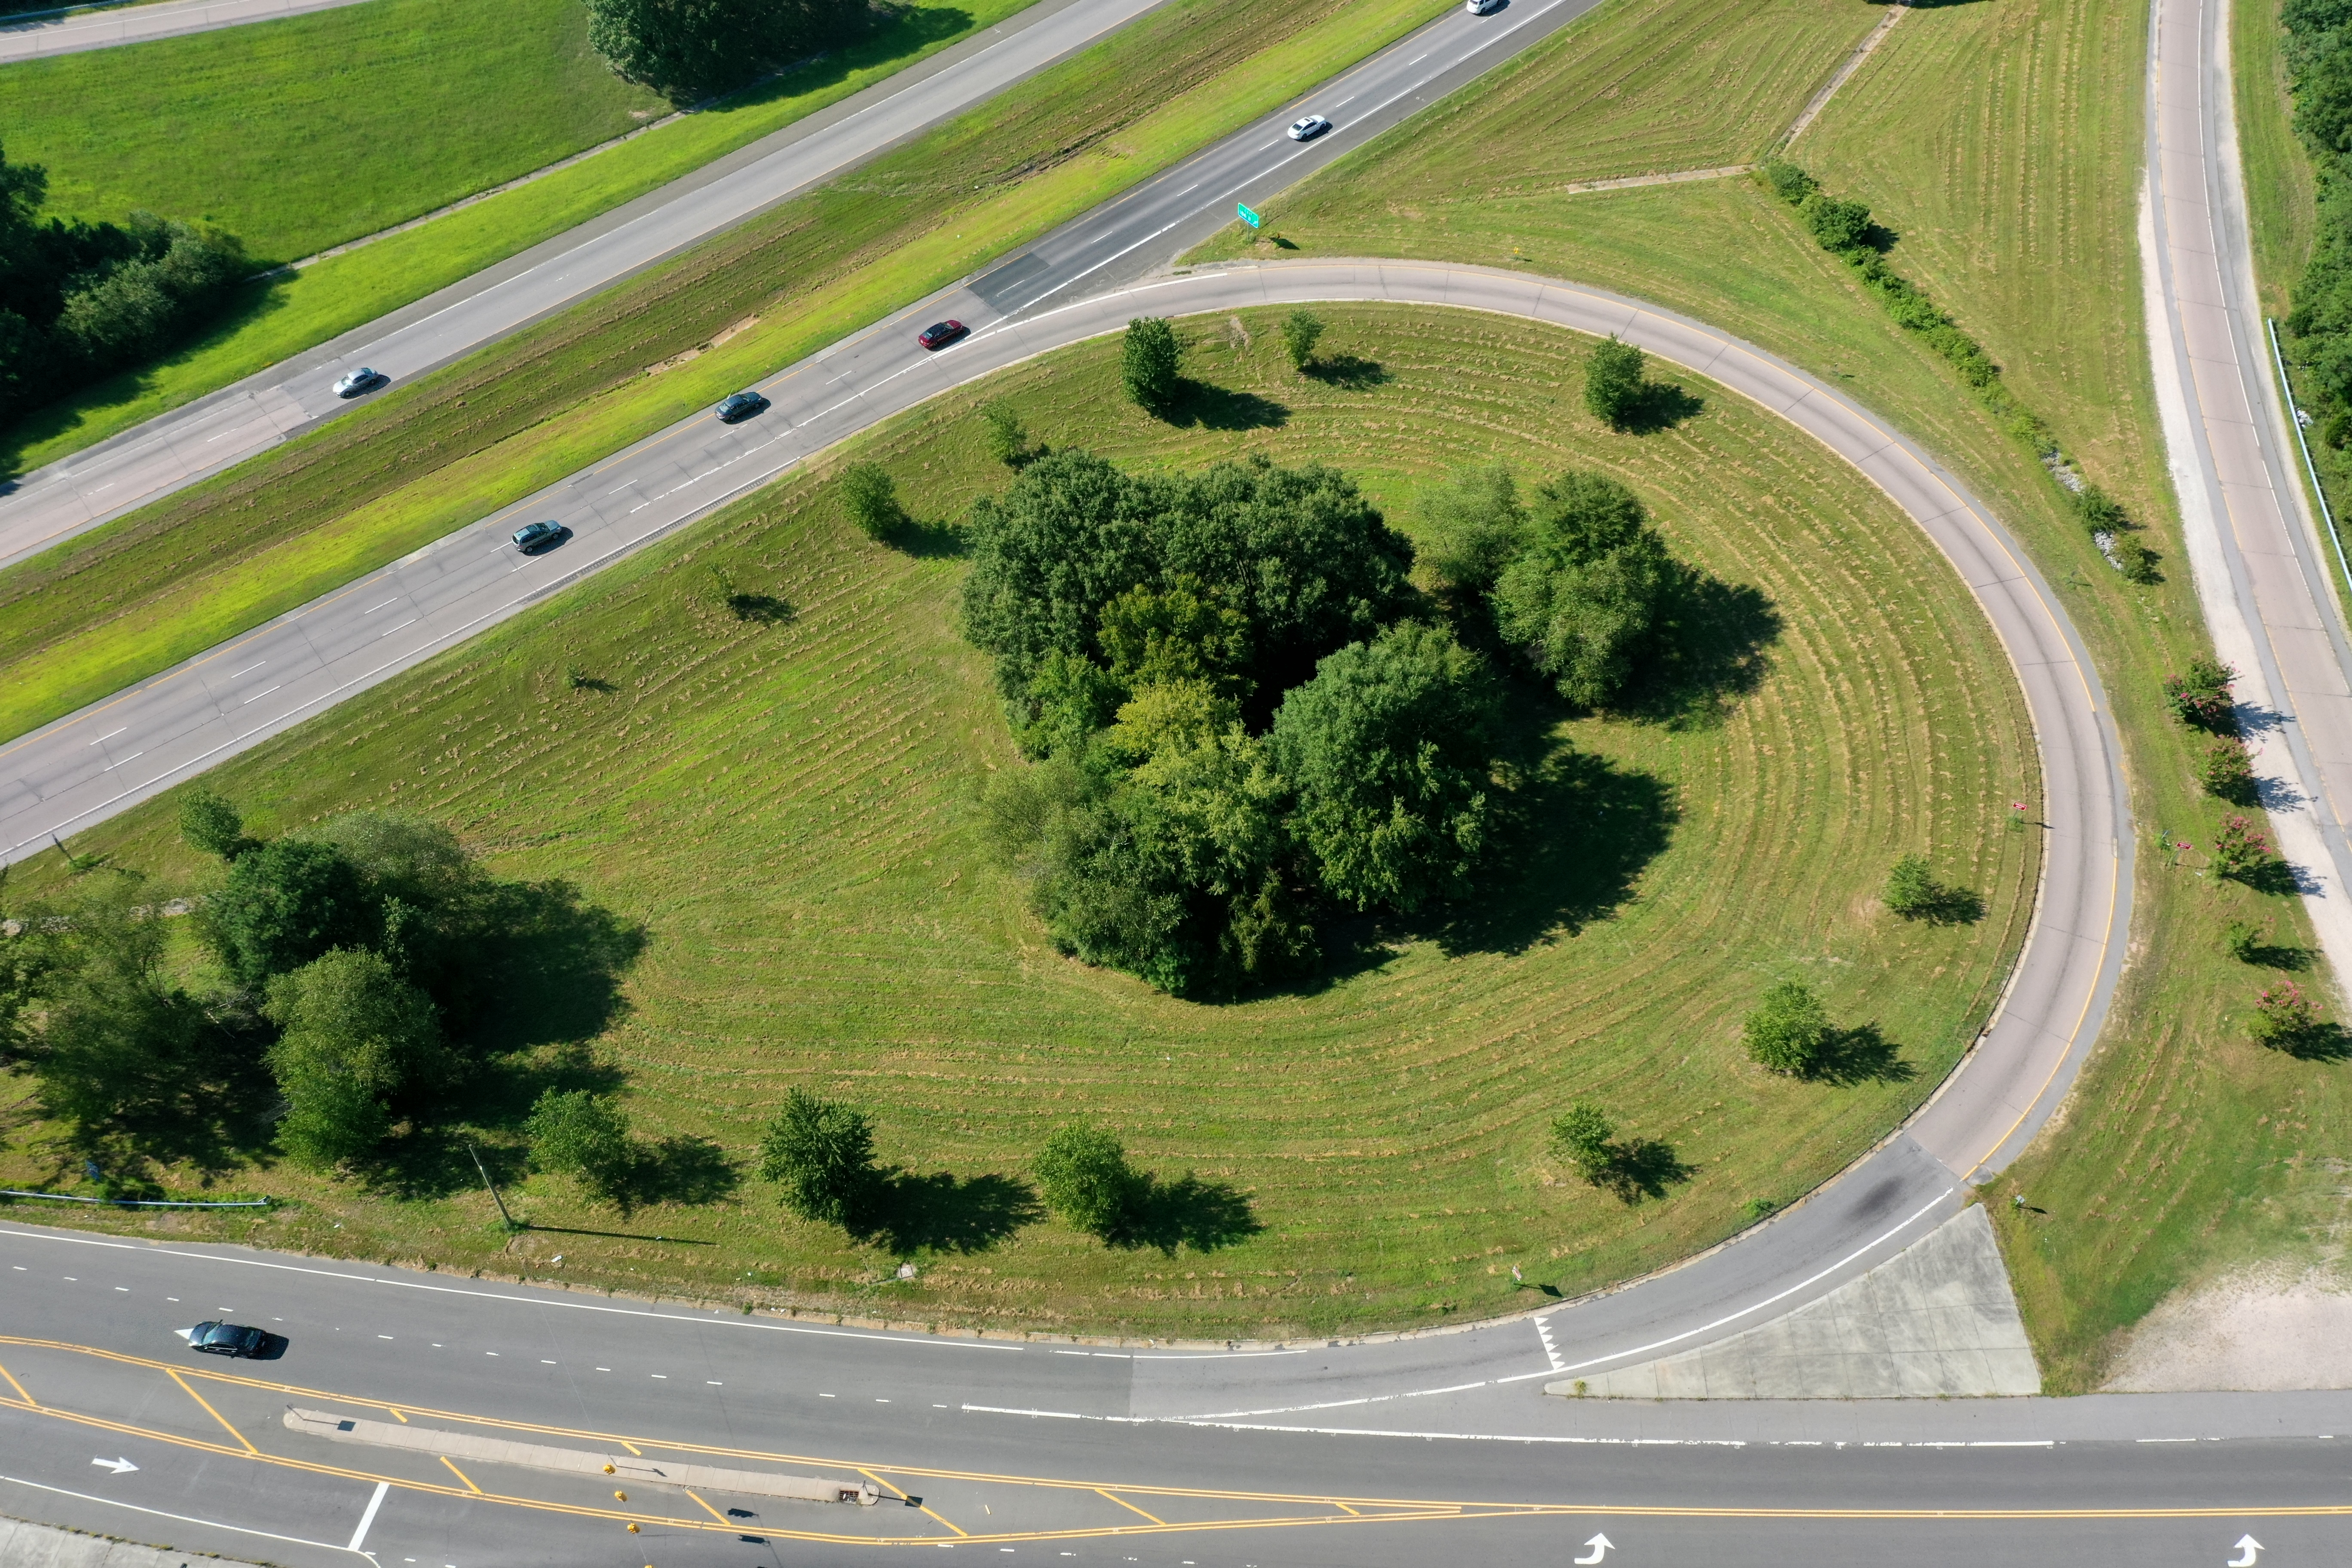
\includegraphics[width=1.0\textwidth]{chapters/Chapitre_3/Figures/onramp.jpg}
\caption{Highway on-ramp}
\label{fig:on-ramp_highway}
\end{minipage}
\label{fig:scenarios_images}
\end{figure}


In this PhD manuscript, our primary focus lies on exploring the manifold potential of MVS in the context of highway scenarios: 
\begin{itemize} % il faut linker ça avec le speed hamonization

\item \textbf{MVS highway navigation in formation:} Autonomous vehicle formation control, akin to broader concept of highway speed harmonization, exerts an important influence on traffic management, yielding numerous benefits such as heightened road safety, optimized traffic flow, and decreased energy consumption. While human-driven vehicles effortlessly navigate in formation, achieving the same behavior for MVS requires a robust and safe strategy to prevent collisions between the vehicles inside and outside the MVS formation. Additionally, the question of MVS formation stability demands a formal \footnote{Formal: by formal, we refer to the existence of an analytical mathematical model.} systematic response. 



Employing a safe and reliable formation control method allows for reduced inter-vehicle spacing within the MVS paradigm, thus optimizing the road capacity utilization. Since vehicles contend with aerodynamic drag that consumes energy, optimizing inter-vehicle distances can mitigate this drag effort, resulting in energy savings as one of the benefits of MVS navigation in formation (cf. Figure \ref{fig:truck_platooning}) \cite{zhao2021distributed}\cite{Mechnical_simulation}. 

\textbf{\begin{figure}[!h]
        \centering 
        \includegraphics[width=9cm,height=18cm,keepaspectratio]{chapters/Chapitre_3/Figures/Co-simulation-in-Matlab-Simulink-TruckSim.png}
        %\vspace{-2.3mm}
        \caption{Truck platooning \cite{zhao2021distributed}}
        \label{fig:truck_platooning}
        %        \vspace{-5mm}
        \end{figure}}

%\newpage

\item \textbf{Cooperative on-ramp merging on highway:} Traffic merging at highway on-ramps presents significant safety and mobility challenges. The complexity emerges when the vehicle on the on-ramp must make split-second decisions regarding acceleration or deceleration to merge safely into the desired highway lane, often without a clear line of sight (cf. Figure \ref{fig:on_ramp_merging_scenario}). Simultaneously, highway road users must adjust their speeds to accommodate the merging vehicle, potentially disrupting traffic flow and leading to congestion (cf. Figure \ref{fig:on_ramp_merging_scenario}). 


\textbf{\begin{figure}[!h]
        \centering 
        \includegraphics[width=9cm,height=18cm,keepaspectratio]{chapters/Chapitre_3/Figures/CooperativeMerging.png}
       % \vspace{-2.3mm}
        \caption{On-ramp merging on highway}
        \label{fig:on_ramp_merging_scenario}
       %         \vspace{-5mm}
        \end{figure}}









To address these challenges, application of cooperative MVS to highway on-ramp merging scenarios can be explored. Various control architectures can be evaluated to their suitability in managing this specific scenario and its associated complexities \cite{7562449}. 



    
\end{itemize}
    As a result, Section \ref{sec: Highway_cooperative_navigation} shows a comprehensive review of the highway cooperative navigation relative application through the Cooperative Adaptive Cruise Control (CACC) (cf. Section \ref{sec: CACC}).  For the problem of cooperative on-ramp merging on highway, Section \ref{sec: cooperative_merging_on_highway} offers a thorough review of relevant approaches. The MVS reviewed application performance are evaluated through the prism of traffic throughput, energy efficiency, and negotiation. 
    
    
    

   % \textcolor{blue}{Discussion: Je ne sais pas si je peux/dois ajouter notre bibio sur les méthodes en relation avec les cooperative intersection crossing ... L'état de l'art est déjà +/- fait, mais dois-je l'ajouter, sachant que ce chapitre est déjà assez long ? }
    %Further insights into the methods used for cooperative intersection crossing are exposed in Section \textcolor{red}{ajouter la section qui parle des méthodes utilisées pour le intersection crossing }. 



% il faut revoir la décomposition des sections pour donner un plus de sens à cela

\subsection{Highway collaborative navigation} \label{sec: Highway_cooperative_navigation}
Collaborative navigation along a highway entails the intricate task of orchestrating the maneuvers of a fleet of vehicles, collectively referred to as MVS in formation navigation in highway, to function as a cohesive unit known as a formation (cf. Section \ref{sec: formation_control_theory}). Advances in communication technology have ushered in the era of V2V communication (cf. Section \ref{sec: communication}), enabling the exchange of information among vehicles within the same formation. 

Traditionally, vehicles on the road tend to follow each other, creating platoon-based formations (cf. Figure \ref{fig:platoon_formation}). For human-operated vehicles, this platoon behavior is a natural occurrence, easily observable in everyday driving scenarios. However, for MVS, adhering to lanes and maintaining safe distances and velocities when following nearby vehicles become more complex endeavor. This complexity arises primarily from the need to effectively manage the dynamics of MVS vehicles, underscoring the requirement for cooperative control over these dynamics.

\textbf{\begin{figure}[!b]
        \centering 
        \includegraphics[width=10.5cm,height=18cm,keepaspectratio]{chapters/Chapitre_3/Figures/cooperative_navigation_in_formation_on_highway}
        %\vspace{-2.3mm}
        \caption{Platoon-based navigation in formation on highway}
        \label{fig:platoon_formation}
             %   \vspace{-5mm}
        \end{figure}}


The primary objective of platoon formation control is to ensure that all vehicles within a platoon travel at the same velocity, adhering to the desired one-dimensional spacial configuration, which is stipulated by a predefined inter-vehicle spacing strategy \cite{jia2015survey}. Consequently, the formation of a platoon-based shape necessitates the development of specialized algorithms, controllers and strategies \cite{mariani2021coordination}. 


In the forthcoming section, we will introduce the concept of Cooperative Cruise Control (CACC) as an important module for executing cooperative navigation maneuvers on the highway. It is proposed in what follows to delve into collaborative navigation within formation and explore its ramifications on highway throughput, energy efficiency and its synergy with negotiation. 


\subsubsection{Cooperative Adaptive Cruise Control (CACC)} \label{sec: CACC}
The core of the CACC concept lies on the fusion of Adaptive Cruise Control (ACC), a subset of automated longitudinal speed control systems, with a cooperative module empowered by the V2V communication and/or V2I communication (cf. Section \ref{sec: communication}) \cite{shladover2015cooperative}.

Over the past decade, considerable advancements in MVS technologies have been achieved. MVS now possess the capability not only to autonomously navigate using onboard sensors but also to communicate with other vehicles via V2V communication. The terms of CACC have been used with varying interpretations, leading to different perceptions of their functions and capabilities in the context of CACC and platooning-based solutions. In CACC systems, MVS exchange their parameters via the V2V communication without a central management unit \cite{wischhof2005information}. Consequently, CACC leverages V2V communication (cf. Figure \ref{fig:platoon_formation}) to enable the vehicles part of the MVS to form platoons and travel at synchronized speed \cite{wang2019survey}. This synchronization is achieved by minimizing the error $d_e$ between the desired distance $d_d$ (depending on the spacing policy and the current dynamic of the MVS) and the current inter-vehicle distance $d_{(.)→(.)}$ (cf. Figure \ref{fig:CACC}). 

        \begin{figure}[h!]
        \centering 
        \includegraphics[width=11cm,height=18cm,keepaspectratio]{chapters/Chapitre_3/Figures/cooperative_adaptive_cruise_control}
       % \vspace{-2.3mm}
        \caption{Cooperative Adaptive Cruise Control}
        \label{fig:CACC}
                %\vspace{-5mm}
        \end{figure}



Through the sharing of vehicle information, including acceleration, speed, and position, MVS with a certain communication range of the roadside unit collaborate to obtain several benefits: 

\begin{itemize}
    \item Enhanced driving safety is achieved through reduced actuation times compared to manual driving, along with improved anticipation of the future actions of the MVS. 

    \item Increased highway capacity results from reduced time/distance headway between the MVS. 

    \item Reduced energy consumption and pollutant emissions stem from minimized unnecessary velocity changes and decreased aerodynamic drag on following vehicles. 
\end{itemize}


        
The vehicle control strategy plays also a role in CACC systems as it determines the vehicle's dynamics. Specifically, the longitudinal control strategy has been extensively studied, \cite{wang2018review}\cite{dey2015review}\cite{nowakowski2010cooperative}, as vehicles operating in CACC mode must maintain the same longitudinal speed as other vehicles in the platoon while sustaining a constant longitudinal distance/headway relative to their preceding vehicle. Various longitudinal controllers have been proposed to address different objectives, such as platoon formation, optimizing fuel consumption, or ensuring system stability \cite{moser2017flexible}\cite{nie2020adaptive}. 

The literature related to the CACC includes several coordination approaches (e.g., consensus-based, optimization-based, etc.). A comprehensive review of these approaches can be found in \cite{wang2018review}\cite{dey2015review}\cite{liu2023systematic}.


One of the objective of this PhD work is take advantage of the MVS advantages (e.g. safety, passenger comfort, energy efficiency). From this perspective, the optimization techniques are well-suited to include these several criteria.  The following sections will undertake an in-depth analysis of various longitudinal controllers founded, based on optimization techniques.


\paragraph{Optimal Control} \label{sec: optimal-control} 
%In addition of MPC, other optimal control methodologies have been explored in the context of CACC. 

Optimal control has been employed to optimize energy consumption or travel time in \cite{massera2017safe}. While many consensus-based control approaches (cf. Section \ref{sec:consensus_control}) focus solely on vehicle speed and position, simplifying the longitudinal control to a single or double integrator model under the assumption of linearity, optimal control techniques often consider non-linearity and constraints \cite{wang2018review}\cite{dey2015review}\cite{shao2017robust}. These constraints may involve vehicle power-train dynamics and aerodynamics \cite{turri2018fuel}. 

In numerous cases where optimal control is applied to CACC systems, the objective function minimizes the total energy consumed by the vehicle traveling within a designated area. For instance, in the Eco-CACC system proposed in\cite{yang2016eco}, it computes the fuel-optimum vehicle trajectory through a signalized intersection, the optimal control problem is defined as: 


\begin{equation}
\min_{a_{-}, a_{+}} \int_{t_{0}}^{t_{0}+T} F(v(t), v'(t)) dt
\end{equation}

subject to

\begin{equation}
\int_{t_{0}}^{t_{0}+T} v(t) dt = d + l
\end{equation}

\begin{equation}
0 \leq a_{-} \leq a_{-}^{s}
\end{equation}

\begin{equation}
0 \leq a_{+} \leq a_{+}^{s}
\end{equation}

Here, $F(\cdot, \cdot)$ represents a nonlinear function of speed $v(t)$ and acceleration $v'(t)$, estimating the energy consumption rate based on vehicular speed and acceleration levels. $a_-$ and $a_+$ are the upstream deceleration and the downstream acceleration levels, respectively. $d$ and $l$ are the length of the control zone before and in the signalized intersection, respectively. 







\paragraph{String stability} \label{sec: string_stability}

String stability is a fundamental requirement to ensure the safety of the CACC system. It aims to attenuate distance error, velocity, or acceleration along the upstream direction in a platoon, as discussed in \cite{rajamani2011vehicle}. The problem of string stability can be formulated as: 

\begin{equation}
|y|{_\infty} \leq|u|{_\infty}
\end{equation}

Here, $y$ represents the scalar output of distance error, velocity, or acceleration of the following vehicle $i+1$, and $u$ represents the scalar output of distance error, velocity, or acceleration of the preceding vehicle $i$. String stability is guaranteed if:

\begin{equation}
\left|\frac{Y(s)}{U(s)}\right|_{\infty} \leq 1
\end{equation}

\noindent where $Y(s)$ and $U(s)$ are the Laplace transforms of $y$ and $u$, respectively.

Numerous works have analyzed the string stability of CACC systems \cite{wang2018review}\cite{nowakowski2010cooperative} \cite{9310215}, and some conclusions have been proposed to ensure string stability: 

\begin{itemize}
    \item If a constant distance spacing policy is adopted for vehicle spacing, the predecessor-follower (cf. Section \ref{sec: communication}) information flow may not guarantee string stability. Extending the information by broadcasting the leader's information to the following vehicles, using a predecessor-follower-leader information flow (cf. Section \ref{sec: communication}), for example, can ensure string stability. 

    \item To relax the formation rigidity imposed by the constant spacing policy, a constant time headway spacing policy can be employed, ensuring string stability by allowing the inter-vehicle distance to depend on the vehicle's velocity \cite{wang2018review}. 
\end{itemize}


\paragraph{Model Predictive Control (MPC): } \label{MPC}
Traditionally, Model Predictive Control (MPC) is framed within the state space framework for single vehicle, where controlled system is described by a linear model as expressed in \cite{stanger2013model}: 
\begin{equation}
\dot{x}(t) = Ax(t) + Bu(t), \quad x(0) = x_{0}
\end{equation}

Here, $x(k) \in \mathbb{R}^n$ represents the state input, and $u(k)\in \mathbb{R}^p$ represents the control input. With $n$ and $p$ are the the state variables and inputs numbers respectively. $A$ is the state matrix, with $dim [A]=n\times n$, and $B$ is the input matrix, with $dim [B]=n\times p$. $x_0$ is the initial state vector. Typically, a receding horizon implementation is formulated as an optimization problem, such as:

\begin{equation}
J_{u(t)}(x_{0}) = \min_{a(t)} \int_{0}^{T} [q_{f}(v(t), a(t)) + \gamma] dt
\end{equation}

Subject to:

\begin{equation}
\Delta \dot{x}(t) = v_{p}(t) - v(t)
\end{equation}

\begin{equation}
\dot{v}(t) = a(t)
\end{equation}

\begin{equation}
\Delta x(t) \geq \Delta x_{\min , 0}+h_{\min } v(t)
\end{equation}

\begin{equation}
\Delta x(t) \leq \Delta x_{\max , 0}+h_{\max } v(t)+\gamma r
\end{equation}

\begin{equation}
a_{\min} \leq a(t) \leq a_{\max }(v(t))
\end{equation}

\begin{equation}
v_{\min} \leq v \leq v_{\max }
\end{equation}

In this context, $q_f$ represents the current fuel consumption depending on $v(t)$ and $a(t)$, where $v(t)$ is the ego-vehicle's velocity and $a(t)$ is its acceleration. $v_{p}(t)$ represents the preceding vehicle's velocity. $\Delta x(t)$ denotes the actual inter-vehicle distance, with $\Delta x_{\min , 0}$ and $\Delta x_{\max , 0}$ being the minimum and maximum distances when stationary. $h_{\min }$ and $h_{\max }$ correspond to the minimum and maximum time headway, associated with the minimum and maximum inter-vehicle distances. The relaxation aspect is introduced through the slack variable $\gamma$ and relaxation parameter $r$. Constraints are also applied to acceleration ($a_{min}$ and $a_{max}$) and velocity ($v_{min}$ and $v_{max}$).


Typically, centralized MPC systems assume knowledge of all the states for computing control inputs. However, in practical applications, especially in dynamic scenarios like highway traffic, gathering information from all the vehicles to compute a large-scale optimization problem is not always feasible. This limitation has led to the development of Distributed Model Predictive Control (DMPC) \cite{caruntu2016distributed}\cite{negenborn2014distributed}, and stochastic MPC (SMPC) to include the uncertainty of the system \cite{moser2015cooperative}.





\subsubsection{Evaluation of the highway collaborative navigation approaches}
As discussed in Section \ref{sec: CooperativeNavigation-Scenarios Overview}, MVS collaborative navigation is linked with several advantages. In this section, an extensive examination of MVS formation navigation in highway is presented, with a focus on aspects such as traffic throughput, energy efficiency, and negotiation.

\paragraph{Traffic throughput} \label{sec: highway_Traffic_throughput}

The primary goal of the CACC systems is to establish and regulate platoon-based formations. Consequently, the advantages of CACC systems can be considered as benefits for formation-based navigation on highways. 

The impact of platoon enabled by CACC on highway throughput was investigated in \cite{van2006impact}. In this research, a stochastic microscopic-traffic simulation model was developed to assess various of traffic flow performance, including safety, exhaust-gas emissions, and noise emissions. The proposed model utilizes real traffic measurements, such as instances, lanes speeds, and vehicle lengths, to generate traffic scenarios at the beginning of simulations runs. The simulations demonstrated that the presence of more CACC-equipped vehicles in traffic leads to higher average velocities. Regarding traffic throughput, scenarios with 100 \% CACC-equipped vehicles showed the best performance compared to other mixing penetration scenarios. 

In \cite{liu2018modeling}, a CACC modeling framework was proposed, incorporating interactions between CACC-equipped vehicles and manually driven vehicles in mixed traffic. This framework included lane-changing rules and automated speed control to ensure realistic CACC performance. Several simulations were conducted on a 4-lanes freeway segment with an on-ramp and off-ramp lanes. The case study compared basic CACC-operated vehicles with Multi-Lanes CACC (ML-CACC)-operated vehicles for different market penetrations. Results indicated that traffic flows with CACC market were consistently lower that those with ML-CACC. 

The study in \cite{jin2020analysis} shows the effect of platooning on mixed traffic and its impact on improving highway throughput. To address this scenario, a new fluid model of mixed-autonomy traffic flow was introduced, which was then used to analyze and design platoon coordination strategies. Simulations were conducted to study the effect of platoon penetration on highway throughput. The results showed that traffic throughput increased with higher platoon fractions on the highway. The study also explored the impact of platoon size, revealing the presence of an optimal platoon size. 


\paragraph{Energy efficiency} \label{sec: energy_efficiency}
Vehicle platooning offers a significant opportunity to enhance energy efficiency by substantially reducing the distance between vehicles, thereby decreasing the aerodynamic drag coefficient \cite{wadud2016help}. The extent of drag reduction in platooning depends on factors such as the vehicle shapes with the platoon, their arrangement, and the distance between them. Savings are most pronounced for vehicles positioned in the middle of the platoon, and the overall savings increase with the number of vehicles in the platoon. For instance, when two vehicles maintain 1-meter gap between them, the average gap reduction is estimated to be around 10 \% \cite{zhu2011simulation}. In cases where the platoon consists of a mix of vehicle types, drag reduction has been estimated at 20\% \cite{schito2012numerical}, and even up to 40 \% \cite{duan2007effects}. In scenarios involving long platoons of vans (five or more vehicles) spaced 0.5 to 1-meters apart, drag reduction of up to 44 \% to 55\% has been reported in \cite{schito2012numerical}. 

Platoon-based formations facilitated by CACC systems also lead to energy efficiency improvements by minimizing unnecessary changes in velocity. In \cite{wang2017developing}, an approach was proposed to minimize energy consumption and pollutant emissions within platoons during various stages, including sequence determination, gap closing and opening, platoon cruising with gap regulation, and platoon joining and splitting. Compared to consensus-based (cf. Section \ref{sec:consensus_control}) CACC system, the results demonstrated that an ECO-CACC (cf. Section \ref{sec: CACC}) could reduce global energy consumption by 1.5 \% during platoon formation and 2 \% during platoon reconfiguration phases \cite{wang2017developing}.

In \cite{bichiou2020vehicle}, an energy consumption model was developed for various types of vehicles, including internal combustion light-duty vehicles, electric vehicles, hybrid electric vehicles, buses and trucks. This model aimed to quantify the effects of platooning on fleet fuel consumption. The findings indicated that energy consumption reductions of up to 3\%, 3.5\%, 4.5\%, 10\%, and 15\%, respectively. 

It becomes evident that vehicles platooning is especially well-suited for heavy-duty vehicles, particularly on highways where travel is at high speeds, leading to substantial aerodynamic drag. Trucks, which often cover long distances on highways, can benefits from joining neighboring trucks to form platoons, even if they have different starting points and destinations. For an in-depth analysis of fuel economy in truck platooning, refer to \cite{zhang2020fuel}. %\textcolor{red}{ajouter des reference sur le truck platooning, ajouter les travaux du gars qui est venus présenter ses travaux au bureau sur platooning}. 

\paragraph{Negotiation} \label{sec: Negotiation_platoon}

To date, the literature lacks of substantial exploration of negotiation- and agreement-based approaches concerning navigation in formation, applied to the case of highways and MVS formation reconfiguration in highway (cf. Figure \ref{fig:negotiation_CACC}) \cite{mariani2021coordination}. This absence may stem from several factors, including unsuitability of such approaches or simply insufficient exploration of these possibilities. One key reason for scarcity of negotiation in this context could be the limited scope for negotiation or discussion with a platoon during cruising. For instance, while one might argue that leader selection could be a negotiation topic, leaders are typically chosen strategically and functionally, often as the vehicle positioned at the front of the formation. Similarly, negotiation speed profiles may not be a significant consideration since the primary goal of a platoon is to travel safely at the maximum allowable speed \cite{mariani2021coordination}. 
\textbf{\begin{figure}[!h]
        \centering 
        \includegraphics[width=11cm,height=18cm,keepaspectratio]{chapters/Chapitre_3/Figures/cooperative_merging_on_highway}
       % \vspace{-2.3mm}
        \caption{Negotiation-based merging in highway}
        \label{fig:negotiation_CACC}
          %      \vspace{-5mm}
        \end{figure}}


However, a potential avenue for exploration is negotiation platoon reconfiguration. Platoon-based formations operate with dynamic environments, such as highways, and are subject to various maneuvers, including vehicles joining, splitting, or changing lanes (individually or as a formation). These maneuvers need to be executed with a global perspective to ensure safety and efficiency, while also being fair in terms of the efforts required from each vehicle. For instance, consider the splitting maneuver depicted in Figure \ref{fig:negotiation_CACC}. Platoon members could engage in discussions where each vehicle proposes its solution to create the desired gap. A negotiation mechanism could then be employed to select the best proposition, taking into account safety and efficiency. 

In practice, scenarios like these are often managed by the platoon leader \cite{amoozadeh2015platoon}. In this work, the authors introduced a platoon management protocol supporting three fundamental maneuvers: merging, splitting, and lane changes. The reconfiguration protocol relies on centralized platoon coordination, where all maneuvers are decided and planned by the platoon leader, and followers follow orders and send requests to and from the leader. However, this approach has limitations associated with centralization (cf. Section \ref{sec:CentralizedArchitecture}), such as restricted flexibility (i.e., typically limited to the communication range) and a lack of formal methods for analyzing the stability of the proposed solutions. 


In addition to the above cooperative highway navigation approaches, on-ramp merging on highway is also one scenario subject to MVS cooperative navigation. The following section presents an overview of the approaches related to MVS on-ramp merging on highway.  
 
\subsection{Collaborative on-ramp merging on highway} \label{sec: cooperative_merging_on_highway}
The merging of traffic at highway on-ramp presents a significant challenge, leading to safety and traffic flow concerns. This challenge becomes particularly pronounced for the merging vehicles, as they must make real-time decisions regarding acceleration or deceleration to safely integrate into the mainlines traffic, often without a clear line of sight. Simultaneously, the drivers on the highway may need to adjust their speeds to facilitate the smooth entry of merging vehicles, potentially, disrupting traffic flow and can induce congestion. In response to these complex issues, researchers have explored the concept of cooperative merging, specifically involving MVS, to address the merging problem at highway on-ramp. 

One can note that the corner stone idea behind collaborative on-ramp merging on highway is to minimize the global effort provided by each vehicle while performing the merging scenario. Naturally, the idea of Prioritizing the stability of the already established vehicle groups (platoons) arises as an evidence. The works in \cite{SCHOLTE2022103511}\cite{s23094401}\cite{9781345} propose several strategies for vehicle merging in an already established platoon with low collaborative efforts.

Various control algorithms have been proposed and implemented to enable the vehicles part of the MVS to merge with one another in a cooperative manner. An extensive review of existing research can be found in \cite{7562449}\cite{awal2013optimal}\cite{zhu2022merging}\cite{bevly2016lane}. In this section, it is proposed to evaluate the existing literature related to cooperative on-ramp merging on-highway through the prism of traffic throughput (cf. Section \ref{sec: on-ramp_traffic_throughput}), energy efficiency (cf. Section \ref{sec: merging_energy_efficiency}), and its implication with negotiation (cf. Section \ref{sec: merging_negotiation}). 

\subsubsection{Traffic throughput} \label{sec: on-ramp_traffic_throughput}
Enhancing highway traffic flow throughput seamless merging at highway on ramps has been a widely explored challenge in the literature. Initially, centralized approaches (cf. Figure \ref{fig:Centralized_merging}) were introduced, utilizing a merging coordinator with support of V2I communication. For instance, in \cite{4047597}, a two-layer centralized controller was proposed based on heuristic rules derived from empirical observations of system behavior. The first layer established the merging sequence by estimating each vehicle's merging time, assuming constant-speed travel. The second layer determined the necessary constant acceleration to resolve conflicts identified during the merging sequence. However, heuristic-based approaches are limited in their adaptability to dynamic environments, and their optimality is not rigorously proven due to the absence of formal optimization algorithms approach. 

\textbf{\begin{figure}[!t]
        \centering 
        \includegraphics[width=10.5cm,height=18cm,keepaspectratio]{chapters/Chapitre_3/Figures/Centralized_cooperative_on_ramp_merging.png}
        %\vspace{-2.3mm}
        \caption{Centralized collaborative on-ramp merging on highway}
        \label{fig:Centralized_merging}
                %\vspace{-5mm}
        \end{figure}}

 %\newpage
To address the optimality concerns in passing sequences, several centralized methods have been developed in the literature, focusing on optimizing travel time to increase highway throughput. These methods use the communication coordinator's responsibility to optimize the passing sequence order based on merging times. An example of optimizing problem formulation is developed below \cite{7562449}, the particularity of this approach resides on reliance on the merging zone crossing time, what makes it less road geometry dependent and more generic: 

\begin{equation}
\min_{u} \frac{1}{2} \sum_{j=1}^{m} \sum_{i=1}^{n}\left[t_{j, i}^{\text {out }}-t_{j, i}^{\text {in }}\right]^{2}
\end{equation}

Subject to: 

\begin{equation}
    \begin{aligned}
\dot{x}_{j, i} &=v_{j, i} \\
\end{aligned}
\end{equation}
\begin{equation}
\begin{aligned}
\dot{v}_{j, i} &=u_{j, i} \\
\end{aligned}
\end{equation}
\begin{equation}
\begin{aligned}
t_{j, i}^{\text {out }}-t_{j, i}^{\text {in }} & \geq \Delta T_{a} \\
\end{aligned}
\end{equation}
\begin{equation}
\begin{aligned}
o<v_{j, i}(t, u) & \leq v^{\max } \\
\end{aligned}
\end{equation}
\begin{equation}
\begin{aligned}
x_{j, i}(t) & \leq x_{j, i+1}(t)+\delta \quad \forall t \\
\end{aligned}
\end{equation}
\begin{equation}
\begin{aligned}
x_{j, i}(t) & \leq x_{p, q}(t)+S \quad \forall t, j \neq p, i \neq q
\end{aligned}
\end{equation}


\noindent where $t_{j, i}^{\text {in }}$ and $t_{j, i}^{\text {out }}$ are the times that the vehicle $i$, on the road $j$, enters and exits the merging zone, $\Delta T_{a}$ is the minimum allowed time to cross the intersection at the maximum speed $v^{\max}$, and $\delta$ is the desired safe distance between vehicles on the same road. $S$ is the length of the shared zone.

Another approach, as presented in \cite{7562449}, offered an optimization framework with an analytical closed-form solution for online vehicle coordination at merging zones. Simulations demonstrated significant reductions in travel times and improvements in traffic flow. In addition, in \cite{chou2016coordinated}, the authors introduced an approach that virtually positioned vehicles onto highway's main lane before actual merging, ensuring smooth and safe merging maneuvers. The results indicated substantial improvements in traffic flow when a high percentage of MVS vehicles were involved. 

\paragraph*{Discussion}
While centralized methods have shown promise in addressing highway on-ramp merging, they come with certain limitations. These approaches heavily rely on communication, exacerbating any communication-related issues that may arise. Moreover, their critical flaw lies in fault tolerance; if the central coordinator fails, the entire system may fail. 

To mitigate these issues, decentralized approaches (cf. Figure \ref{fig:Decentralized_merging}) can be considered. These approaches draw inspiration from centralized methods, such as the concept of virtual vehicles/platooning. 

\textbf{\begin{figure}[!h]
        \centering 
        \includegraphics[width=10.5cm,height=18cm,keepaspectratio]{chapters/Chapitre_3/Figures/Cooperative_on_ramp_merging.png}
       % \vspace{-2.3mm}
        \caption{Decentralized collaborative on-ramp merging on highway}
        \label{fig:Decentralized_merging}
           %      \vspace{-5mm}
        \end{figure}}
In the virtual vehicle/platooning approach, each merging vehicle communicates its position and velocity within a certain range. Based on this data, each vehicle constructs its view of the merging scenario, replacing real-vehicles with virtual ones. Passing orders are then generated individually by each vehicle part of the MVS, aided by the virtualization. Conflict checks are performed to prevent merging collisions, with adjustments made if conflicts arise, depending on the merging strategy. An advanced variation of this approach introduced the concept of slots\footnote{ A slot is a geometrical space in the highway mainline, defined by its coordinates w.r.t. a common reference frame within the MVS, usually used by the vehicle for negotiation purposes to avoid collision}, allowing the vehicles part of the MVS to navigate within virtual slots. Conflict checking is conducted across these slots, accommodating localization uncertainties and ensuring minimal safety distances \cite{6338779}. In comparison with centralized methods, this cooperative merging method demonstrated superior performance in terms of traffic throughput and average on-ramp vehicle delay. %However, the level of conservativeness can vary based on slot dimensions, with slot-based virtual vehicle/platooning potentially being more conservative than the centralized approaches. 

\subsubsection{Energy efficiency} \label{sec: merging_energy_efficiency} 
Merging onto a dense highway from an on-ramp presents a complex challenge, characterized by its combinatorial nature and the limited information available regarding average speed in the different lanes \cite{7265166}. Additionally, ramp merging often leads to congestion and the formation of phantom traffic jams\footnote{Phantom traffic jams: dense traffic crawls to a halt for no apparent reason.} \cite{VAHIDI2018822}. V2V communication (cf. Section \ref{sec: communication}) offers a solution by enabling the anticipation of neighboring vehicles' intentions. This advanced knowledge of lane speeds can enhance the eco-driving control algorithms of MVS \cite{VAHIDI2018822}, resulting in more informed and smoother merging maneuvers. According to \cite{7313484} \cite{7562449}, these improvements can lead to an increased energy efficiency. Moreover, the benefits may extend beyond individual vehicles; by reducing the occurrence of phantom jams, the overall energy efficiency of traffic can be enhanced. However, it is worth noting that very few works have explored this particular advantage of MVS coordination on merging \cite{VAHIDI2018822}. %This scarcity of research can be attributed to the challenges associated with estimating fuel consumption, which is a complex task, and the intricate nature of on-ramp merging scenarios. Table \ref{energy} provides a summary of the limited findings regarding the impact of cooperative on-ramp merging on energy efficiency.


% \begin{table}[!ht]
% \renewcommand\arraystretch{1.25}
% \begin{adjustwidth}{-0.1\textwidth}{-0.1\textwidth}
% \caption{\label{energy}Summary of selected published results on energy efficiency gain enabled by anticipating margining on-ramp on highway.}
% \begin{tabularx}{\linewidth}{c c c } 
% \hline
% %\lipsum[11]\leavevmode\vspace*{-\baselineskip}
%  Reference &  Method and conditions & Energy efficiency (gain in \%)  \\ [0.8ex] 
%     \hline %%%%%%%%%%%%
%      \begin{minipage}{0.25\textwidth}   \vskip \cite{kamal2011ecological}  \vskip \end{minipage} &\Longstack{  \begin{minipage}{0.50\textwidth}   \vskip \begin{itemize} \setlength\itemsep{-0.4em} \item MPC velocity controller with $15\text{s}$ as prediction horizon  \end{itemize} \vskip  \end{minipage}} & \begin{minipage}{0.15\textwidth} \vskip  \empty{}\\\begin{itemize} \setlength\itemsep{-0.4em} \end{itemize} \vskip \end{minipage} \\  
%      \begin{minipage}{0.15\textwidth}   \vskip   \vskip \end{minipage} &\Longstack{  \begin{minipage}{0.50\textwidth}   \vskip \begin{itemize} \setlength\itemsep{-0.4em}  \item Simulation scenarios in $2\text{Km}$ road distance:  \subitem At $50\%$ MVS equipped with MPC controller w.r.t. conventional vehicles  \subitem At $50 \%$ MVS equipped with Cooperative Adaptive Cruise Control (CACC) w.r.t. conventional vehicles  \end{itemize} \vskip  \end{minipage}} & \begin{minipage}{0.15\textwidth} \vskip  \begin{itemize} \setlength\itemsep{-0.4em} \item $+12.9$ \\ \item $+7.5$  \end{itemize} \vskip \end{minipage} \\ 
%      \hline

%      %%%%%%%%
%      \begin{minipage}{0.25\textwidth}   \vskip \cite{7534837}  \vskip \end{minipage} &\Longstack{  \begin{minipage}{0.50\textwidth}   \vskip \begin{itemize} \setlength\itemsep{-0.4em} \item Optimal control based approach  \end{itemize} \vskip  \end{minipage}} & \begin{minipage}{0.15\textwidth} \vskip  \empty{}\\\begin{itemize} \setlength\itemsep{-0.4em} \end{itemize} \vskip \end{minipage} \\  
%      \begin{minipage}{0.15\textwidth}   \vskip   \vskip \end{minipage} &\Longstack{  \begin{minipage}{0.50\textwidth}   \vskip \begin{itemize} \setlength\itemsep{-0.4em}  \item Simulation scenarios:  \subitem  Coordination of $30 \text{vehicles}$ with same initial speed \subitem  Coordination of $30 \text{vehicles}$ With Different Initial Speed for Each Road \end{itemize} \vskip  \end{minipage}} & \begin{minipage}{0.15\textwidth} \vskip  \begin{itemize} \setlength\itemsep{-0.4em} \item $+52.7$ \\ \item $+48$  \end{itemize} \vskip \end{minipage} \\ 
%      \hline

%      %%%%%%%%
     
     
    
     
%     \hline

% \end{tabularx}
% \end{adjustwidth}
% \end{table}
% \\






\subsubsection{Negotiation} \label{sec: merging_negotiation}
In the absence of road coordinator and predefined heuristic rules, a vehicle seeking to merge into a lane from an on-ramp vehicle must ensure two conditions: (a) avoiding collisions with vehicles already in the targeted lane, and (b) executing a smooth merge without abruptly slowing down the vehicles on the target lane \cite{mariani2021coordination}. 

The approaches proposed in \cite{amoozadeh2015platoon} and \cite{aoki2017merging} rely on V2V communication (cf. Section \ref{sec: communication}) through the Vehicular Ad-Hoc network VANET protocol to facilitate negotiation. The merging vehicle initiates action proposals to vehicles already on the target lane, with the latter having the right to decline and propose alternative actions. In congested traffic conditions, such approaches are susceptible to issues of resource allocation, as vehicles on the highway may be unwilling or unable to accept proposals of cooperation from on-ramp vehicles. In other terms, the allocation of resources (space and time) for vehicles willing to merge from on-ramps to highway can be problematic due to reluctance or inability of vehicles already on the highway to accept this merging proposals. 

To address the challenge of resource allocation, negotiation approaches based on incentive mechanisms can be conceptualized. For instance, merging vehicles could employ auctions \cite{adhau2012multi}\cite{adnan2016protocols}\cite{cui2013game},where they offer compensation to enter the target lane. However, as of now, no relevant examples of such mechanisms have been found in the literature.


\section{Conclusion}


This chapter introduced various paradigms employed in the construction of the multi-vehicles system (MVS) control architecture. Additionally, it delved into the concept of formation control through a comprehensive review of the diverse approaches utilized for this purpose. Furthermore, this chapter explored the relevant literature concerning the versatile application of MVS, where the main challenges related to the different applications were highlighted. 

Addressing the challenges of MVS in dynamic and complex on-road environment, such as on-ramp merging and navigation in formation in highway, requires a multifaceted control architecture. The key takeaways from this chapter are listed as follows: 









\begin{enumerate}

    \item \textbf{Formal modeling of the MVS formation:} The formation composed by the vehicles part of the MVS should be done following a formal approach. Formal modeling helps to prove the stability of the formation motion, provides safety proofs, and enhances the cooperation efficiency. 

    \item \textbf{Distributed solution:} The proposed solution should aim for a high degree of decentralization to minimize dependencies on central units.

     \item \textbf{Promoting cooperation:} To prevent selfish behaviors, negotiation mechanisms should be an integral part of the solution to encourage cooperative interactions. Additionally, the notion of altruism coupled with MVS cooperation can be interesting to mitigate this issue. 

    
     \item \textbf{Performance demonstration:} The effectiveness of the proposed solution should be demonstrated in through the prism of its effects on safety, traffic flow, passenger comfort, and energy efficiency. 

    \item \textbf{Robustness:} The decision-making layer must prioritize robustness to ensure safe operations, and risk management methods should be integrated to maintain collision-free interactions.

     \item \textbf{Uncertainty assessment:} Recognizing that uncertainties are inherent to the problem, the proposed solution should incorporate mechanisms to address these uncertainties effectively.


\end{enumerate}

%% ajouter les deux références ci dessous à la partie navigation en formation dans le highway avec le concept de platoon virtuel 
% - W.J. Scholte, P.W.A. Zegelaar, H. Nijmeijer,
%A control strategy for merging a single vehicle into a platoon at highway on-ramps,Transportation Research Part C: Emerging Technologies, Volume 136,

% - Yongjie Xue, Xiaokai Zhang, Zhiyong Cui, Bin Yu, Kun Gao,
%A platoon-based cooperative optimal control for connected autonomous vehicles at highway on-ramps under heavy traffic, Transportation Research Part C: Emerging Technologies, 


























% l'idée de cette section est de donner des exmples d'application de la navigation en formaiton des MVS 
% \subsection{MVS navigation in formation: an application review}
% In the realm of MVS, the utilization of advanced formation methodologies has become pivotal in addressing a myriad of complex challenges mainly related to MVS' motion coordination. In particular, Cooperative Cruise Control (CACC) and consensus-base control strategies attention for their potential to improve the dynamics of MVS coordination. Building upon the fundamental concepts (cf. Section \ref{sec: formation_control_theory}), this section explores the multifaceted applications of CACC and consensus-based control within the realm of MVS. Through a comprehensive examination, it is proposed to delve into the intricacies of these control paradigms, shedding light to their promising contributions to enhancing on-road safety and transportation efficiency.







% Mes éléments c'est les suivants: 
% - navigation in formation  (application in highway - Leader follower, consensus based control) 
% - stategies used for on-ramp and off-ramp merging 
% - stategies used to MVS motion coordination - intersection crossing and roundbout 

  % PART 2
  \part{Cooperative Multi-Controller Architecture}
  % TOC 
% introduction 
% problem statement -- on peut parler de la problème générale & dans le chapitre sur la structure virtuelle on peut parler de backround and challenges pour présenter ce qui existent dans la structure virtuelle et ce qu'on veut faire avec cette strcture
% Goals of the proposed architecture (AFRS)
% OVerall AFRS architecture 
% Conclusion 

% Goals of this chapter 
% The gloabl context of the thesis was largely presented before - 
% Now, we want to present the achitecture used for the thesis 
% Present the global idea of the formation reconfiguration using the virtual structure and how it can be used to tackle the scenario of on-ramp merging on highway 
% Present the decision making level and it is used/connected to the rest of the architecture 


% il faut un contexte générale à cette partie tout en sachant 

\chapter{The proposed Cooperative Multi-Controller Architecture (C-MCA)}

\label{Chap03}
\begin{abstract}
    In this Chapter an global overview of the proposed Cooperative Multi-Controller Architecture (C-MCA). Drawing inspiration from the foundational multi-controller architecture, a brief summary of the latter is presented. Subsequently, the chapter delves into the key functionalities of the C-MCA, with a particular focus on decision-making and planning at the system level. The chapter concludes with a dedicated section addressing the problem statement related to the this PhD work.

    
\end{abstract}


\textbf{Contents}
\vspace{0.15cm}
\hline
\hspace{2cm}
\localtableofcontents
\hspace{2cm}
\hline




 \section{Introduction}


The overarching goal of this PhD work centers on building a decision/control architecture that takes advantage from the MVS coordination ability to overcome the challenges related to on-ramp merging on highway. Consequently, two main sub-objectives related to the decision/control were identified: (1) Developing a suitable approach for MVS navigation in formation for on-ramp merging on highway, and (2) Build a decision-making level designed to mitigate the on-ramp merging challenges. 

 
The examination of the MVS paradigm and its associated control architectures in Chapter \ref{chap:chapter1} and Chapter \ref{chap:chapter2} have led to the realization that classical control architectures come with inherent limitations. Keeping the idea of building a decision/control architecture suitable for MVS on-ramp merging on highway, while mitigating the classical control architecture limitations. This chapter delves into the proposed Cooperative Multi-Controller Architecture (C-MCA). 




The C-MCA is based on the foundational multi-controller architecture, consequently, Section \ref{sec:MCA} elaborates the multi-controller architecture background relevant to this PhD work. Section \ref{sec: AFRS} presents an overview of the proposed Cooperative Multi-Controller Architecture (C-MCA).  Lastly, section \ref{sec: problem_statement} outlines the problem statement tackled in this work. 





\section{Multi-controller architecture} \label{sec:MCA}



The principal aim of the Multi-Controller Architecture (MCA) is to systematically decompose the fundamental functions of the MVS, in order to break down the complexity of the tackled scenario. In essence, it endeavors to disassemble the overarching task into a sequence of sub-tasks. Consequently, implementing the MCA necessitates the development of reliable elementary controllers and specialized mechanisms, often referred to as behaviors, to proficiently manage their interactions. 

The MCA, depicted in Figure \ref{fig:MCA}, serves as the foundational framework for our research. Its purpose is to oversee interactions among elementary behaviors while upholding the overall control system's stability, as discussed in \cite{dimiathesis}. The MCA, featured in Figure \ref{fig:MCA}, primarily encompasses three elementary behaviors: lane keeping, adaptive cruise control and lane change. It is pertinent to highlight that the underlying operational principals of three two behaviors have been extensively expounded upon in the literature (cf. Chapter \ref{chap:chapter2}). Our particular interest lies in the adaptation of the behavioral concept for MVS on-ramp merging on highway navigation, as well as, the selection process part of the decision-making of the MCA in Figure \ref{fig:MCA}. 

During each sampling interval, one of these three behaviors is activated via a the behavior selection mechanism (cf. Figure \ref{fig:MCA}) part of the decision-making level based on inputs from the perception, localization and communication modules. Each vehicle's controller consists of a dedicated and uniform set of way-points, defined by pose  $X_T=[x_T, y_T, \theta_T]$ and the desired velocity $v_T$. It is crucial to underscore that, once these target points are established, the controllers must rely on robust control laws to consistently reach and track these designated target points. 

        \begin{figure}[!h]
        \centering 
        \includegraphics[width=11cm,height=18cm,keepaspectratio]{chapters/Chapitre_4/Figures/Adapted_control_architecture.png}
       % \vspace{-2.3mm}
        \caption{Multi-Controller Architecture}
        \label{fig:MCA}
       % \vspace{-5mm}
        \end{figure}







Building upon the MCA paradigm outlined in this section, the subsequent section provides an overview of the main functionalities of the proposed C-MCA tailored for merging onto highway on-ramps in the context of MVS. Special attention is given to the decision-making and planning levels.




% Cooperative Navigation (CN) stands as a widely adopted approach to ensure the effective maneuvering of intelligent vehicles within complex/cluttered environments. As discussed in Section \ref{sec: CooperativeNavigation-Scenarios Overview}, the coordination complexities arising in both rural and urban settings encompass tasks such as harmonizing speeds on motorways and highways, facilitating smooth merging on on-ramps, and orchestrating the movements of the vehicles on highways. However, the primary hurdle lies in accurately assessing and mitigating potential hazards within the road environment while implementation adaptable CN strategies, as discussed in Section \ref{sec: CooperativeNavigation_GlobalOverview}. Consequently, the main aim of this Ph.D. thesis is to propose a safe and energy efficient control architectures for MVS that navigates in dynamic and complex environment such as merging on on-ramp and multi-road navigation on highway,  with a reasonable communication conditions. 

% % il faut parler du contenue de ce chapitre en précisant les items qui y figurent 
% More precisely, this chapter firstly outlines in Section \ref{sec: problem_statement} the the general problem statement tackled in this PhD along with the main related challenges. The global decision/control architecture proposed in the context of this PhD is given in Section \ref{sec: AFRS}. 



















\section{Overall Cooperative Multi-Controller Architecture} \label{sec: AFRS}

% pour l'architecture proposée on peut citer les items suivants: 
% - commencer par la partie architecture global avec les modules mais d'un point de vu global 
% - dire que les modules perceptions et localization sont déjà traités avant dans les sections et les citer 
% - mettre l'ascent sur les architectures multi-controller et les systèmes de selection de comportement (switch, etc) 
% - introduire notre propre architecture, et expliquer les modules et leurs fonctionnement ! 


\subsection{The C-MCA main functionalities}






The primary focus of this work revolves around adapting the MCA detailed in Section \ref{sec:MCA}, to suit the requirements of cooperative navigation within the MVS paradigm in complex and dynamic environments. More precisely, it is proposed to employ the MCA as the foundational framework in the development of a Cooperative Multi-Controller Architecture (C-MCA) (cf. Figure \ref{fig:C-MCA}) designed to overcome the challenges related to MVS navigation on on-ramp merging and cooperative highway navigation. 

The proposed C-MCA is depicted in Figure \ref{fig:C-MCA}. It has been designed around various interconnected modules that facilitate planning, control, access, and management of on-ramp merging and cooperative highway navigation within MVS. This section aims to establish a global focus of the main functionalities part of the C-MCA, whith an emphasis on the decision-making level (cf. Figure \ref{fig:C-MCA} \textcircled{\small{1}}) and the local trajectory planning (cf. Figure \ref{fig:C-MCA} \textcircled{\small{2}}).  























\subsubsection{Environment perception} \label{sec:environment_features}
As discussed in both Section \ref{sec: perception} and Section \ref{sec: localization}, the roles of the perception and localization modules involves furnishing the essential environmental characteristics indispensable for MVS navigation. These characteristics encompass critical information such as the vehicle's precise localization, the number of lanes, lane markings, distances to road boundaries, and the pose of detected obstacles. To achieve this, these modules operate based on a vector map, serving as a detailed representation of the environment. Fusion algorithms, combining data from perception and localization, are employed to generate a reliable representation of the environment. 


\textbf{\textit{Assumption 1:}} It is essential to underscore that this PhD manuscript concentrates on the decision-making and planning/control modules with the C-MCA. Consequently, the perception, localization, and vector map modules are assumed to be reliable and are not the primary focus of this research.  





\newpage
\thispagestyle{empty}
\begin{landscape}
        \begin{figure}[!h]
        \centering 
        \includegraphics[width=20cm,height=18cm,keepaspectratio]{chapters/Chapitre_4/Figures/C_MCA.png}
        \vspace{-2.3mm}
        \caption{Cooperative Multi-Controller Architecture }
        \label{fig:C-MCA}
        \vspace{-5mm}
        \end{figure}


\end{landscape}
















\subsubsection{Communication module} \label{sec:communication_module}
  This module operates in collaboration with the Road Side Unit (RSU) positioned within the merging zone (cf. Figure \ref{fig:ScenarioTopology}). The RSU acts as a conduit for the exchange of crucial information between the merging vehicle and the highway vehicles, thus enhancing of the MVS's motion coordination capabilities. In essence, when referring to the communication aspect of this research, it pertains to the exchange of information between the vehicle components of the MVS and the RSU, all within the communication range defined in Figure \ref{fig:ScenarioTopology}. Further details related to the RSU can be found in Appendix \hyperlink{AppendixA}{A}). 

\textbf{\textit{Assumption 2:}} It is important to note that the communication module, both within the vehicles and integrated into the RSU, functions as tools aimed at enhancing the overall abilities of the MVS.  However, it is crucial to acknowledge that the complexities inherent in the levels addressed in this research preclude the comprehensive investigation of communication-related aspects such as communication delays, packet losses, and dynamic communication topologies. 
















\subsubsection{Global path planning}\label{sec:global_planner} 
The global path planner module gives a selected sequence of way-points through the road network. Additionally, it has the responsibility of setting the goal of the vehicle (e.g., its destination, navigating lane, etc.). It uses the inputs of the perception modules to cope with the traffic road rules 
(e.g., speed limits, traffic signs, etc.).










% \subsubsection{Risk assessment and management module} \label{sec:risk_assessment} 
% The principal objective of the risk assessment and management module is to uphold the paramount safety criterion consistently. This module has been devised to interpret the environment feature data and determine whether the decision-making level possesses the capacity to ensure compliance with safety criterion. In cases where such assurance is lacking, this module can trigger a fail-safe procedure. 








\subsubsection{Decision-making level} \label{sec:decision_making}
After defining the environmental perception and the vehicle's global path, it becomes imperative to adopt an appropriate decision-making strategy for the vehicle component within the C-MCA. This strategy must consider various factors, including the vehicle's objectives, the MVS overarching objectives, traffic regulations, etc. 



The core requirement of the decision-making level is to ensure the safety of the MVS during the on-ramp merging maneuver. Consequently, given the shared nature of on-ramp merging scenario and the high dynamic relative to the highway, the decision-making must establish a strategy to solve the conflicting scenarios. Before delving into the presentation of the proposed decision-making level part of the C-MCA, a short overview of the literature approaches used to solve the conflicts part of the shared zones is proposed.



As with intersection crossing, the merging conflict is mainly justified because of the shared nature of the merging zone \cite{mariani2021coordination}. Thus, solving conflicting scenarios requires an appropriate strategy designed to take into account explicitly these conflicting configurations. Several strategy can be found in the literature and they can be mainly classified in two categories:  (1) Centralized approaches and Decentralized approaches. In Centralized approaches, a Central controller defines the passing sequence of the vehicle in the shared zone, and the vehicles have no words concerning the selection policy. In contrast, in decentralized approaches, negotiation-based strategy can be used to establish the passing sequence. Some contributions part of the intersection crossing and on-ramp merging literature focused on the competitive nature of the  scenario \cite{mariani2021coordination}. Thus, the use of negotiation can be performed with auction-based mechanism. While approaching the shared zone, each vehicle can contact the RSU and place a bid; place an offer to buy a portion of the shared zone for a certain period. The value of the bid expresses the urgency of the vehicle. The RSU collects the bids and accord the conflict portion to the vehicle that placed the highest bid \cite{carlino2013auction}\cite{cabri2019auction}\cite{vasirani2012market}. The main limitation of the auction-based strategy is the liveness of the method, i.e., as explained in  \cite{mariani2021coordination} liveness stands for starvation of the vehicles; in some cases, the constant bidding strategy of the vehicle can prevent other vehicles from wining an auction, with the risk for them an indefinitely waiting time. 



        \begin{figure}[!h]
        \centering 
        \includegraphics[width=12cm,height=18cm,keepaspectratio]{chapters/Chapitre_4/Figures/Decision-making-level.pdf}
       % \vspace{-2.3mm}
        \caption{Flowchart of the decision-making level part of the C-MCA}
        \label{fig:Decision-module}
        %\vspace{-5mm}
        \end{figure}



In this PhD work, instead of relying on the competitive nature of the on-ramp merging scenario, it is proposed to rely on its cooperative nature. Consequently, the conflicting is solved while ensuring the respect of the MVS overarching goal and vehicle's individual goals. The decision-making level within the C-MCA module is founded upon a multi-behaviors decision-making system. This decision-making module (cf. Figure \ref{fig:C-MCA} \textcircled{1}) is responsible for selecting one of the two operational behaviors within the local trajectory level (cf. Figure \ref{fig:C-MCA} \textcircled{2} and Figure \ref{fig:Decision-module}), with respect to the safety criterion. In simpler terms, the decision-making level prompts the nominal behavior (responsible for promoting the vehicle's individual goals) to make predictions about the vehicle's expected nominal motion (cf. Figure \ref{fig:Decision-module} and Figure \ref{fig:C-MCA} \textcircled{2}). Based on these predictions, the safety criterion is assessed, if the nominal behavior is safe then the latter is activated. However, when a conflicting merging is detected based on the nominal behavior, the decision-making level and the cooperative behavior works together to solve the conflict (cf. Figure \ref{fig:Decision-module} and Figure \ref{fig:C-MCA} \textcircled{1} \textcircled{2}), while respecting both the MVS overarching goal and the vehicle's  individual goals. Further details about the multi-behavior decision-making level part of the C-MCA can be found in Chapter \ref{Chap05}. 





















\subsubsection{The local trajectory planning level} \label{sec:local_planning}
The local trajectory planning level part of the C-MCA in Figure \ref{fig:C-MCA} is composed of two primary behaviors: 

\begin{enumerate}
\item The nominal behavior: It takes into account data from the environment perception, and global path planning modules to predict the expected behavior of each vehicle within the MVS. The nominal behavior is designed to achieve the MVS vehicle's individual goals, thus it is optimized to enhance the performance of the involved vehicle. The forecaster behavior is subsequently evaluated using a safety metric by the decision level within the C-MCA, further details can be found in Section \ref{sec:The_nominal_mode}. 

\item The cooperative behavior: In cases where the nominal behavior fails to adhere to the safety criterion, the C-MCA decision-making level activates the cooperative behavior. Consequently, the cooperative behavior receives additional inputs, including safety evaluations related to the nominal behavior, in addition to the selected passing sequence. Based on these inputs, the cooperative behavior has the responsibility of generating the vehicles' dynamics corresponding to the passing sequence. The translation of the passing sequence into the MVS dynamics is ensured by the formation control strategy part of C-MCA.  Further details about the formation control strategy are given in Chapter \ref{Chap04}. 




\end{enumerate}






\subsubsection{The control level} \label{sec:control_law}
The control level is tasked with the precise tracking of the set-points generated by the local planning level. These set-points serve as a reference for the control to follow. The local trajectory planning level creates a velocity profile and yaw rate that are well-suited for the vehicle.

The used control law is the one detailed in Section \ref{sec:control_law}. The control law is synthesized for a tricycle model-based vehicle (cf. Section \ref{sec:control_law}) using Lyapunov  synthesis and is detailed in Section \ref{sec:control_law}. 



% je ne sais pas s'il faut ajouter une phrase de transition ici ou pas ... 


\section{Problem statement} \label{sec: problem_statement}
% ajouter une partie ou on parle du scenario qu'on cherche à traiter dans cette thèse avec toute la topologie de la route etc. Un peu comme le fait déjà zhang enfaite :! -- voir mon carnet de notes 
% il faut aussi présenter les hypothèses de travail qu'on fait tout au long de cette thèse comme celle sur la communication par example ! 
% il faut aussi expliquer comment la communication intervient dans l'architecture et comment les tâches sont distribuées entre les différents véhicules etc 





As previously discussed in both Chapter \ref{chap:chapter2} and Chapter \ref{Chap03}, and as highlighted by the comprehensive literature reviews in  \cite{bernardin2019scenario} \cite{guo2019urban} \cite{wang2019survey} \cite{7562449}, the coordination challenges confronting MVS extend their influence over a wide array of environments, encompassing both rural and urban settings, including highways. These challenges manifest in a multitude of scenarios, including the imperative for coordination on highways to maintain uniform speeds, as well as the intricacies of merging onto and exiting from on-ramps. As elucidated in Section \ref{sec: CooperativeNavigation-Scenarios Overview}, the cooperative navigation of MVS on highways ushers in an array of driving benefits, ranging from enhancing safety to improved traffic flow and optimized energy efficiency (cf. Section \ref{sec: CooperativeNavigation-Scenarios Overview}). 


In this section, we aim to provide an overview of the background that underlies this PhD thesis. Section \ref{sec:ScenarioTopology} will present a representation of the highway scenario involving on-ramp, thereby establishing the overarching road topology that serves as the foundational scenario of this work. Subsequently, the control law used in this PhD work is detailed. Lastly, the formalism definition and modeling of the formation are discussed. 


\subsection{Scenario topology}\label{sec:ScenarioTopology}

This research endeavors to leverage the capabilities of MVS to confront the intricacies associated with cooperative highway navigation. More precisely, it sets out to address the challenging scenario of cooperative merging at highway on-ramps, a scenario associated with significant safety and mobility complexities. The specific use at the heart of this research is illustrated in Figure \ref{fig:ScenarioTopology}, encompassing a multi-lane highway environment incorporating an on-ramp as the entry point to the highway section. Additionally, this scenario accounts for a designated merging zone, characterized by a fixed length, where merging maneuvers are authorized. Furthermore, the prescribed speed limits governing both the highway and the on-ramp segments are integrated as predetermined parameters with this scenario. 



        \begin{figure}[!h]
        \centering 
        \includegraphics[width=12.5cm,height=18cm,keepaspectratio]{chapters/Chapitre_4/Figures/ScenarioScene.pdf}
        \vspace{-2.3mm}
        \caption{Illustration of the scenario topology of the on-ramp merging on highway}
        \label{fig:ScenarioTopology}\label{fig:RSU-identification}
       % \vspace{-5mm}
        \end{figure}




The distinctive feature of the on-ramp merging scenario is the complex motion synchronization hurdles encountered by the vehicles. These challenges materialized as vehicles on the on-ramp must make decisions about whether to accelerate or decelerate. All this, while ensuring a safe and continuous merge onto the desired highway lane, often under conditions where a clear line of sight is not guaranteed. Simultaneously, highway users must adapt their speeds to accommodate to the behavior of the merging vehicle, which can potentially disrupt the flow of traffic and result in congestion. One way to help synchronization ability of the vehicles participating in the merging scenario is with the help of communication. In this work, we take the assumption of a on-ramp merging scenario equipped with a Road RSU (cf. Appendix \hyperlink{AppendixA}{A}).  


\subsection{Control law } \label{sec:control_law}

Before presenting the used control law, it is important to know the vehicle's model. 



Assuming that the vehicle evolves in asphalt road and in cluttered urban environment with relatively low speed, the following model is based on tricycle model \cite{ventura2015safe}. The two front wheels are replaced by a single virtual wheel located at the center of both front wheels. 


\begin{equation} \label{eq:vehiclemodel}
\begin{aligned}
\dot{x} &=v \cos (\theta) \\
\dot{y} &=v \sin (\theta) \\
\dot{\theta} &=v \tan (\gamma) / l_{b}
\end{aligned}
\end{equation}

\noindent $(x,y,\theta)$ is the vehicle's pose on the global reference frame $X_{G},Y_{G}$. $v$ is the vehicle's linear velocity and $\gamma$ is the steering angle of the vehicle. $l_{b}$ is the vehicle's wheelbase. $v$ and $\gamma$ are the control inputs of the vehicle (cf. eq \ref{eq:vehiclemodel}). 



	\begin{figure}[!h]
	\begin{center}
		
		\includegraphics[width=120mm,height=80mm]{chapters/Chapitre_4/Figures/vehicle_tricycle model.PNG}\\
		\caption{	\label{fig:vehicle_tricycle_model}Vehicle’s and target’s configuration in global $(X_G; Y_G)$ and local $(X_m; Y_m)$ reference
frames, and the control variables \cite{ventura2015safe}}
		
		
		
	\end{center}
\end{figure}



According to Figure \ref{fig:vehicle_tricycle_model}, $w_b$ corresponds to the track width of the vehicle and $I_{cc}$ the instantaneous center of curvature of the vehicle trajectory. The radius of curvature $r_c$ is given by: 

\begin{equation}
    r_c=\frac{l_b}{tan(\gamma)}
\end{equation}

\noindent and $cc=1/r_c$ is the curvature of the vehicle trajectory. \\




The used control law \cite{vilca2015novel} aims to drive the vehicle toward specific targets (static or dynamic) in the environment. At each sample time the tracked target is defined by a posture $(x_T,y_T,\theta_T$) and velocity ${V}_T$ (this velocity could be equal to 0 if the target is static). Using a Lyapunov formulation, the used control law \cite{vilca2015novel} is presented below. 

The adopted Lyapunov function $V$ is given by eq. \ref{eq:lay_control_1}. 

\begin{equation}\label{eq:lay_control_1}
\begin{aligned}
V & =\frac{1}{2} K_d d^2+\frac{1}{2} K_l d_l^2+K_o\left[1-\cos \left(e_\theta\right)\right] \\
& =\frac{1}{2} K_d d^2+\frac{1}{2} K_l d^2 \sin ^2\left(e_{R T}\right)+K_o\left[1-\cos \left(e_\theta\right)\right]
\end{aligned}
\end{equation}


\noindent where the initial values of $e_{R T}$ and $e_\theta$ must satisfy the following initial conditions:
\begin{equation}
    e_{R T} \in ]-\pi / 2, \pi / 2\left[\text { and } e_\theta \in \right]-\pi / 2, \pi / 2[
\end{equation}

The Lyapunov function (cf. eq. \ref{eq:lay_control_1}) is therefore a function of three parameters which depend on: the distance $d$ between the target and vehicle's position; the distance $d_l$ from the vehicle to the target line (line that passes through the target position with an orientation equal to the target orientation), this term is related to the Line of Sight and Flight of the target; and the orientation error $e_\theta$ between the vehicle and the target.


The desired linear velocity $v$ and the front wheel steering $\gamma$ of the vehicle which allow to asymptotically stabilize the error vector $\left(e_x, e_y, e_\theta,\left(v-v_T\right)\right)$ toward zero (permitting therefore to have $\dot{V}<0$) are given by:

\begin{equation}
\begin{aligned}
v & =v_T \cos \left(e_\theta\right)+v_b \\
\gamma & =\arctan \left(l_b c_c\right)
\end{aligned}
\end{equation}

\noindent where $v_b$ and $c_c$ are defined by: 
\begin{equation}
v_b=K_x\left[K_d e_x+K_l d \sin \left(e_{R T}\right) \sin \left(e_\theta\right)+K_o \sin \left(e_\theta\right) c_c\right]
\end{equation}
with: 
\begin{equation}
\begin{aligned}
c_c= & \frac{1}{r_{c_T} \cos \left(e_\theta\right)}+\frac{d^2 K_l \sin \left(e_{R T}\right) \cos \left(e_{R T}\right)}{r_{c_T} K_o \sin \left(e_\theta\right) \cos \left(e_\theta\right)}+K_\theta \tan \left(e_\theta\right) \\
& +\frac{K_d e_y-K_l d \sin \left(e_{R T}\right) \cos \left(e_\theta\right)}{K_o \cos \left(e_\theta\right)}+\frac{K_{R T} \sin ^2\left(e_{R T}\right)}{\sin \left(e_\theta\right) \cos \left(e_\theta\right)}
\end{aligned}
\end{equation}

\noindent $K=(K_d, K_l, K_o, K_x, K_\theta, K_{RT})$ is a vector of positive constants defined by the designer. Accurate analysis of this stable and efficient control law is given in \cite{vilca2015novel}\cite{ventura2015safe}. 

\subsection{Formation definition and configuration}\label{sec:formation_modeling_section}







Based on the MVS paradigm (cf. Section \ref{sec:MVS-paradigm}) and the communication range of the RSU (cf. Figure \ref{fig:ScenarioTopology}), a set of $N$ vehicles involved in creating the formation is identified. In other words, the RSU establishes connections with all the vehicles within its communication range. Consequently, the RSU assigns a unique communication identifier, in addition to the definition of the reference vehicle used as a reference frame by the formation coordinate system. This strategy is defined as follows: 

\begin{itemize}
    \item \textbf{Reference vehicle:} The RSU has the responsibility of designating the reference vehicle $V_R$ (cf. Figure \ref{fig:RSU-identification}). The pose of the latter is used as a mobile reference frame by the formation coordinates system. The RSU can select $V_R$ either from the vehicles part of the MVS or by considering a virtual vehicle. In this thesis work, the reference vehicle $V_R$ is selected from the MVS vehicles traveling in the lane containing the merging zone, and based on the shortest distance w.r.t. merging zone (cf. Figure \ref{fig:RSU-identification}). Its position is denoted by $x_{\text{R}}, y_{\text{R}}$, and its velocity by $\mathcal{V}_{\text{R}}$.
    
    
 

    \item \textbf{Formation modeling approach:} The formation of MVS is structured based on the virtual structure approach (cf. Section \ref{sec: Virtual-structure}). Figure \ref{fig:Coordinates_system} presents the formation coordinates  $F={f_i,i=1,\ldots,N}$, where $f_i$ are the $i-th$ vehicle coordinates w.r.t. the reference frame of the formation. 

    
% \end{itemize}
%        \begin{figure}[!h]
%         \centering 
%         \includegraphics[width=14cm,height=6cm]{chapters/Chapitre_5/Figures/RSU_identification.pdf}
%         %\vspace{-2.3mm}
%         \caption{Formation identification and id attribution}
%         \label{fig:RSU-identification}
%         %\vspace{-5mm}
%         \end{figure}





\subsubsection{Formation modeling based on a dynamic reference frame}


In Figure \ref{fig:RSU-identification}, the RSU broadcast $V_{R}$ pose to the vehicles part of the formation in order to compute their coordinates w.r.t. $V_R$ reference frame. According to \cite{8430659}, two suitable frames for formation definition can be used: 


\begin{itemize}
    \item \textbf{Cartesian reference frame:} also called rigid formation, it aims to maintain the formation's shape, the positions and orientations of the vehicles within the formation, computed relative to $V_{R}$, which is also called the leader vehicle, with respect to the Cartesian reference frame (the local frame of the reference vehicle defined as $X_m$ and $Y_m$). This approach aims to reduce vehicle's dependence on a global reference frame. Applying a straightforward transformation allows the determination of the vehicles part of the formation coordinates within a local reference frame attached to the reference vehicle \cite{mariottini2007leader}\cite{benzerrouk2010navigation}.

    \item \textbf{Frenet reference frame:} \label{sec:FrenetFrame} also known as flexible formation, this approach is utilized when it is more critical to track the reference vehicle's movements than to maintain a fixed formation shape during navigation. The Frenet reference frame is employed to adapt the formation to the reference vehicle's trajectory. This trajectory is used to define the formation's longitudinal (curvilinear) and lateral (perpendicular to the trajectory) coordinates \cite{8430659}\cite{avanzini2010urban}\cite{klanvcar2011control} (cf. Figure \ref{fig:Coordinates_system}).
\end{itemize}








In the Cartesian formation, the reference vehicle path is not taken into account such as in the Frenet formation, only its current Cartesian pose and dynamics have to be known by the vehicles part of the formation. Since the reference vehicle trajectory is part of the Frenet formation modeling, the latter offers a safe formation navigation in static environment. In contrary, according to \cite{8430659}, the Cartesian formation allows a safe stable geometric formation shape. 

During the on-ramp merging scenario, the formation shape is reconfigured from one initial shape to another, while guaranteeing the safety of the reconfiguration. Based on the advantages of both of the formation modeling approaches, the Frenet modeling approach is the one that satisfies the scenario requirements. In fact, one of the particularities of the on-road environment is its high dynamic, especially for highway environment. Additionally, the Frenet modeling approach offers more flexibility, an important requirement for navigation in dynamic environments. 

\subsubsection{Formation modeling based on the Frenet reference frame}
Each vehicle part of the formation is characterized by its coordinates $X_i=[x_i,y_i]^T$ within the global reference frame $[X_G,Y_G]$ (cf. Figure \ref{fig:Coordinates_system}). In order to locate $X_i$ w.r.t. the reference vehicle $V_R$ (cf. Figure \ref{fig:Coordinates_system}), it is proposed to use a Frenet reference frame (cf. Section \ref{sec:FrenetFrame}) centered on $V_R$ (cf. Figure \ref{fig:Coordinates_system}). 

       \begin{figure}[!h]
        \centering 
        \includegraphics[width=12.5cm,height=18cm,keepaspectratio]{chapters/Chapitre_5/Figures/ModelingScenarioSimple.pdf}
        %\vspace{-2.3mm}
        \caption{Coordinates system based on the Frenet reference frame}
        \label{fig:Coordinates_system}
        %\vspace{-5mm}
        \end{figure}



According to $V_R$ pose $X_R$ and its reference trajectory (cf. Figure \ref{fig:Coordinates_system}), the coordinates system is described as follows: 

\begin{itemize}
    \item The $i-$vehicle coordinates part of the formation are defined as $f_i=[h_i,l_i]^T, i\in {N}$ (cf. Figure \ref{fig:Coordinates_system}). 

    \item $h_i$ and $l_i$ are the longitudinal and lateral vehicle's coordinates w.r.t. the Frenet reference frame, respectively. The longitudinal coordinate $h_i$ represents the curvilinear distance between $V_R$ and $X_i$ according to the tangent to $V_R$ trajectory, while the lateral coordinate $l_i$ is computed based on the perpendicular line between $X_R(h_i)$ and its reference trajectory, and that passes through $X_i$, $l_i=PerpDist{X_R(h_i),X_i}$ (cf. Figure \ref{fig:Coordinates_system}). 
\end{itemize}


The kinematic model in eq. \ref{eq:vehiclemodel} is written in the global reference frame ${X_G, Y_G}$, thus a transformation from the mobile reference frame to the global reference frame is obtained with the following equations: 

\begin{equation} \label{eq:frenetToCartisian}
\begin{matrix}
\begin{bmatrix}
x_{T_i} \\
y_{T_i} \\
\end{bmatrix}
& = & \begin{bmatrix}
x_{R}(h_i)\\
y_{R}(h_i) \\
\end{bmatrix}
& + & \begin{bmatrix}
-l_i\sin(\theta_R(h_i)) \\
l_i\cos(\theta_R(h_i)) \\
\end{bmatrix}
\end{matrix}
\end{equation}


with $[x_{T_i},y_{T_i}]^T$ is the i-th vehicle virtual target w.r.t. $V_R$'s mobile reference frame. $[x_R,y_R]^T$ and $\theta_R$ are the reference vehicle $V_R$ pose and orientation.



       % \begin{figure}[!h]
       %  \centering 
       %  \includegraphics[width=14cm,height=6cm]{chapters/Chapitre_5/Figures/Full_scenario.png}
       %  %\vspace{-2.3mm}
       %  \caption{The virtual structure approach used to model the formation and its reconfiguration to perform the merging maneuver. (a) The initial shape of the formation and its coordinates. (b) The final shape of the formation after the merging maneuver and its desired coordinates. }
       %  \label{fig:Coordinates_system_full_scenario}
       %  %\vspace{-5mm}
       %  \end{figure}











\section{Conclusion}

This chapter presented the design of the Cooperative Multi-Controller Architecture (C-MCA) for safe and energy efficient on-ramp merging on highway, in addition to the details given on the main modules, as well as, their interactions. Indeed, the C-MCA aims to satisfy both the MVS overarching goal and the vehicle's individual goals. With the help of the multi-behavior decision-making level part of the architecture, the nominal behavior is activated when it is safe to satisfy the vehicle's individual goals. Satisfying the vehicle's goals is not always possible, especially given the shared nature of the merging zone. Consequently, the C-MCA has a dedicated cooperative behavior that works along the negotiation protocol part of the decision-making level to solve conflicting merging scenarios. In fact, a safe passing sequence is selected by the decision-making level, and the latter is translated into the vehicle's dynamics by the formation control approach part of the cooperative behavior. The following chapter is dedicated to present the details related to the proposed formation control strategies. 
  %!TEX root = ../Thesis.tex

\chapter{Dynamic Formation Reconfiguration for On-Ramp Merging}
%\addcontentsline{toc}{part}{Introduction} % Adds "Introduction" as part-style in ToC
%\markboth{Introduction}{Introduction}    % Marks left and right headers as "Introduction"

\label{Chap04}
\begin{abstract}
In scenarios involving conflicting mergings, the decision-making component of the C-MCA is tasked with determining a secure passing sequence for the MVS within the merging zone. The passing sequence is subsequently translated into the MVS dynamics in the planning level through the application of the formation reconfiguration mechanism. Within this chapter, several dynamic formation reconfiguration approaches for on-ramp merging will be discussed. Each proposed formation reconfiguration will be outlined, and its performance will be assessed to identify any limitations. These identified limitations will then guide the refinement of the formation reconfiguration mechanism, iteratively improving it until the planning objectives of the C-MCA are satisfactorily met\footnote{The detailed contributions in this chapter have been the subject of the following publications \hyperlink{ITSC22}{ITSC'22}, \hyperlink{VAMS23}{VAMS'23},  \hyperlink{MMAR23}{MMAR'23} and  \hyperlink{ITSC23}{ITSC'23}.}.
\end{abstract}


\textbf{Contents}
\vspace{0.15cm}
\hline
\hspace{2cm}
\localtableofcontents
\hspace{2cm}
\hline












% In order to overcome the challenges related to the problem of on-ramp merging (cf. Section \ref{} \textcolor{red}{ajouter la reference de la section ou on parle de la complexité du on-ramp merging}), one consider the tackled scenario as a formation control problem. In other terms, the vehicles aiming to perform the merging maneuver as well as the highway can be seen as members of the same formation. Consequently, the formation need to be defined and configured, modeled, and perform the merging maneuver through the formation reconfiguration. 







% \subsection{Formation definition and configuration}\label{sec:formation_modeling_section}







% Based on the MVS paradigm \textcolor{red}{ajouter la reference de la section qui parle de l'état de l'art sur le MVS paradigm dans le chapitre 1} and the communication range of the RSU \textcolor{red}{ajouter la reference de la section qui parle des RSU ici}, a set of $N$ vehicles involved in creating the formation are identified. In other words, the RSU establishes connections with all the vehicles within its communication range. Consequently, the RSU assigns a unique communication identifier, in addition of the definition of the reference vehicle used as a reference frame by the formation coordinate system. This strategy is defined as follows: 

% \begin{itemize}
%     \item \textbf{Reference vehicle:} The RSU has the responsibility of designating the reference vehicle $V_R$ (cf. Figure \ref{fig:RSU-identification}). The pose of the later is used a mobile reference frame by the formation coordinates system. The RSU can select $V_R$ either from the vehicles part of the MVS or by considering a virtual vehicle. In this thesis work, the reference vehicle $V_R$ is selected from the MVS vehicles traveling in the lane containing the merging zone, and based on the shortest distance w.r.t. merging zone (cf. Figure \ref{fig:RSU-identification}). Its position is denoted by $x_{\text{R}}, y_{\text{R}}$, and its velocity by $\mathcal{V}_{\text{R}}$.
    
    
 

%     \item \textbf{Formation modeling approach:} The formation of MVS is structured based on the virtual structure approach (cf. Section \ref{} \textcolor{red}{ajouter la reference de la structure virtuelle}. In Figure \ref{fig:Coordinates_system} presents the formation coordinates  $F={f_i,i=1,\ldots,N}$, where $f_i$ are the $i-th$ vehicle coordinates w.r.t. the reference frame of the formation. 

    
% \end{itemize}
%        \begin{figure}[!h]
%         \centering 
%         \includegraphics[width=14cm,height=6cm]{chapters/Chapitre_5/Figures/RSU_identification.pdf}
%         %\vspace{-2.3mm}
%         \caption{Formation identification and id attribution}
%         \label{fig:RSU-identification}
%         %\vspace{-5mm}
%         \end{figure}





% \subsubsection{Formation modeling based on a dynamic reference frame}


% In Figure \ref{fig:RSU-identification}, the RSU broadcast $V_{R}$ pose to the vehicles part of the formation in order to compute there coordinates w.r.t. $V_R$ reference frame. According to \cite{8430659}, two suitable frames for formation definition can be used: 


% \begin{itemize}
%     \item \textbf{Cartesian reference frame:} also called rigid formation, it is to maintain the formation's shape, the positions and orientations of the vehicles within the formation are computed relative to $V_{R}$, which also called the leader vehicle, with respect to the Cartesian frame (the local frame of the reference vehicle defined as $X_m$ and $Y_m$). This approach aims to reduce vehicle's dependence on a global reference frame. Applying a straightforward transformation allows the determination of the vehicles part of the formation coordinates within a local reference frame attached to the reference vehicle \cite{mariottini2007leader}\cite{benzerrouk2010navigation}.

%     \item \textbf{Frenet reference frame:} \label{sec:FrenetFrame} also known as flexible formation, this approach is utilized when it is more critical to track the reference vehicle's movements that to maintain a fixed formation shape during navigation. The Frenet reference frame is employed to adapt the formation to the reference vehicle's trajectory. This trajectory is used to define the formation's longitudinal (curvilinear) and lateral (perpendicular to the trajectory) coordinates \cite{8430659}\cite{avanzini2010urban}\cite{klanvcar2011control} (cf. Figure \ref{fig:Coordinates_system}).
% \end{itemize}








% In the Cartesian formation, the reference vehicle path is not taken into account such as in the Frenet formation, only its current Cartesian pose and dynamic have to be known by the vehicles part of the formation. since the reference vehicle trajectory is part of the Frenet formation modeling, the latter offers a safe formation navigation in static environment. In contrary, according to \cite{8430659}, the Cartesian formation allows a safe stable geometric formation shape. 

% During the on-ramp merging scenario the formation shape is reconfigured from one initial shape to another, while guaranteeing the safety of the reconfiguration. Based on the advantages of both of the formation modeling approaches, the Frenet modeling approach is the one that satisfy the scenario requirements. In fact, one of the particularities of the on-road environment is their dynamic, especially for highway environment. Additionally, the Frenet modeling approach offers more flexibility, an important requirement for navigation in dynamic environments. 

% \subsubsection{Formation modeling based on the Frenet reference frame}
% Each vehicle part of the formation is characterized by its coordinates $X_i=[x_i,y_i]^T$ within the global reference frame $[X_G,Y_G]$(cf. Figure \ref{fig:Coordinates_system}). In order to locate $X_i$ w.r.t. the reference vehicle $V_R$ (cf. Figure \ref{fig:Coordinates_system}), it is proposed to use a Frenet reference frame (cf. Section \ref{sec:FrenetFrame}) centered on $V_R$ (cf. Figure \ref{fig:Coordinates_system}). 

%        \begin{figure}[!h]
%         \centering 
%         \includegraphics[width=14cm,height=18cm,keepaspectratio]{chapters/Chapitre_5/Figures/ModelingScenarioSimple.pdf}
%         %\vspace{-2.3mm}
%         \caption{Coordinates system based on the Frenet reference frame}
%         \label{fig:Coordinates_system}
%         %\vspace{-5mm}
%         \end{figure}



% According to $V_R$ pose $X_R$ and its reference trajectory (cf. Figure \ref{fig:Coordinates_system}) the coordinates system is described as follows: 

% \begin{itemize}
%     \item The $i-$vehicle coordinates part of the formation are defined as $f_i=[h_i,l_i]^T, i\in {N}$ (cf. Figure \ref{fig:Coordinates_system}). 

%     \item $h_i$ and $l_i$ are the longitudinal and lateral vehicle's coordinates w.r.t. the Frenet reference frame, respectively. The longitudinal coordinate $h_i$ represents the curvilinear distance between $V_R$ and $X_i$ according to the tangent to $V_R$ trajectory, while the lateral coordinate $l_i$ is computed based on the perpendicular line between $X_R(h_i)$ and its reference trajectory, and that passes through $X_i$, $l_i=PerpDist{X_R(h_i),X_i}$ (cf. Figure \ref{fig:Coordinates_system}). 
% \end{itemize}


% The kinematic model in eq. \ref{eq:kinematic model} \textcolor{red}{voir ou est le soucis avec cette equation} is written in the global reference frame ${X_G, Y_G}$, thus a transformation from the mobile reference frame to the global reference frame is obtained with the following equations: 

% \begin{equation} \label{eq:frenetToCartisian}
% \begin{matrix}
% \begin{bmatrix}
% x_{T_i} \\
% y_{T_i} \\
% \end{bmatrix}
% & = & \begin{bmatrix}
% x_{R}(h_i)\\
% y_{R}(h_i) \\
% \end{bmatrix}
% & + & \begin{bmatrix}
% -l_i\sin(\theta_R(h_i)) \\
% l_i\cos(\theta_R(h_i)) \\
% \end{bmatrix}
% \end{matrix}
% \end{equation}


% with $[x_{T_i},y_{T_i}]^T$ is the i-th vehicle virtual target w.r.t. $V_R$'s mobile reference frame. $[x_R,y_R]^T$ and $\theta_R$ are the reference vehicle $V_R$ pose and orientation.



  






\section{Introduction}




The key concept behind the proposed dynamic formation reconfiguration approach is to take advantage of the MVS coordination ability to achieve safely and smoothly the merging scenario. In other terms, dynamic formation reconfiguration is used to control the vehicles motion during the merging phase. 

Once the ${N}\in \mathbb {N}$ vehicles part of the formation are identified, the Frenet frame (cf. Section \ref{sec:FrenetFrame}) is used to model the initial shape $F^{init}$. The formation desired shape $F^{end}$ (cf. Figure \ref{fig:Coordinates_system_full_scenario}) is obtained through the translation of the passing sequence $sq$ selected by the decision-making level. Lastly, in order to perform the merging maneuver, the formation reconfiguration process is launched. 

     \begin{figure}[!h]
        \centering 
        \includegraphics[width=13cm,height=6cm]{chapters/Chapitre_5/Figures/FullMergingScenario.pdf}
        %\vspace{-2.3mm}
        \caption{The virtual structure approach used to model the formation and its reconfiguration to perform the merging maneuver. (a) The initial shape of the formation and its coordinates. (b) The final shape of the formation after the merging maneuver and its desired coordinates. }
        \label{fig:Coordinates_system_full_scenario}
        %\vspace{-5mm}
        \end{figure}

Formation reconfiguration is the process that reshapes the formation from its initial shape $F^{init}$ toward the final one $F^{end}$ by generating intermediary formation coordinates $F(t)$ (cf. Figure \ref{fig:Coordinates_system_full_scenario}). The intermediary coordinates are transformed from the Frenet frame to the global Cartesian frame to generate the vehicles virtual targets $T_d$. The respect of the merging safety is ensured with the help of the inter-vehicle target distances. In other terms, each vehicle part of the MVS has its own virtual target $T_d$ generated by the formation reconfiguration process. The distance between two targets is the inter-vehicle target distances. Consequently, the MVS safety during the merging is ensured by the generation of safe virtual targets. The system of equations that describes the formation reconfiguration are given below: 
    


\begin{equation}\label{eq:initialandfinalcoordinates}
\begin{cases}
F^{init}=[f_{1}^{{init}^T}, ...,f_{N}^{{init}^T}]^T, \\
F^{end}=[f_{1}^{{end}^T}, ...,f_{N}^{{end}^T]^T},\\
F(t)=[f_{1}(t)^T, ...,f_{N}(t)^T]^T,
\end{cases}
\end{equation}

$f_i ^{init},f_i ^{end}, i\in {N}$ are the coordinates of $V_i$ in the initial and final formation, while $f_{i}(t), i\in{N}$ are its instantaneous coordinates. 

$e_{f_{i}}=[e_{h_{i}},e_{l_{i}}]^T $ is the convergence error between the desired coordinates of $V_i$ in the formation and the actual ones, it can be defined as: 

\begin{equation}\label{eq: errorbetweenfinitandfendforvi}
\begin{cases}
    e_{f_{i}}=f_{i}^{end} - f_{i}(t),\\
    f_{i}(t)=[h_{i}(t), l_{i}(t)]^T,\\
    f_{i}^{end}=[h_{i}^{end},l_{i}^{end}]^T,
\end{cases}
\end{equation}

The global error for a formation composed of ${N}$ vehicles can be written as: 
\vspace{-2.3mm}
\begin{equation}
    e_{F}=F^{end} - F(t)
\end{equation}

The derivative expression of the error can be written as: 
\begin{equation} \label{eq:fct error}
    \dot{e}_F=g(e_{f_{1}}, ..., e_{f_{N}})
\end{equation}


Equation \ref{eq:fct error} describes the formation reconfiguration problem as a control problem, where the goal is to control the convergence error from its initial value (error with the initial formation shape) toward the final one (error with the desired shape, so zero), while ensuring the respect of the vehicles' safety. 

 Part of this research work, several formation reconfiguration approaches were proposed. The following sections aim to describe these approaches. In Section \ref{sec:CORM}, the Constrained Optimal Reconfiguration Matrix (CORM) is described along with its advantages and limitations. Based on the CORM's limitations, the Extended Constrained Optimal Reconfiguration Matrix (E-CORM) was proposed (cf. Section \ref{sec:E-CORM}). Lastly, in order to overcome both the CORM's and the E-CORM's limitations, the Formation Reconfiguration Approach based on an Online Control Strategy (FRA-OCS) is proposed and presented in Section \ref{sec:No-opt}. The performance of each of the proposed formation reconfiguration approaches is discussed with the help of several simulation results. 





    
 \section{Constrained Optimal Reconfiguration Matrix (CORM)} \label{sec:CORM}  



The proposed Constrained Optimal Reconfiguration Matrix (CORM) involves an analysis of the derivative of $e_F$ (cf. eq. \ref{eq:fct error}). This analysis aims to ensure convergence to the new formation shape and generates smooth trajectories using the virtual targets during the reconfiguration process. Additionally, it helps to manage the minimum inter-target distance to prevent collisions between vehicles. 

The CORM is originally inspired by the inter-target distance matrix, thus, a concise overview of the latter is presented in the following section. Subsequently, the section focuses on the Constrained inter-target distance matrix proposed to explicitly take into account the road constraints. Lastly, this section delves into the safe and feasible local trajectory planning strategy proposed to ensure the feasibility of the formation reconfiguration during the merging. 



\subsection{The inter-target distance matrix} \label{sec:Inter-target-distance-matrix}

The proposed function $\dot{e}_F$ for the entire formation is adapted from \cite{ventura2015safe}\cite{8430659}, and it is designed as a linear system: 

\begin{equation}\label{eq:linearSystem}
    \dot{e}_{F}= Ae_F
\end{equation}

where $e_F=[e_{f_{1}}^T, ..., e_{f_{N}}^T]^T$ and $A^{2N \times 2N}$ are the state vector and the inter-target distance matrix corresponding to a formation of $N$ vehicles, respectively. 

\begin{equation}\label{eq: reconfiguration matrix}
A = 
 \begin{bmatrix}
  a_{1}I^{2 \times 2} & a_{12}I^{2 \times 2} & \cdots & a_{1N}I^{2 \times 2} \\
  -a_{12}I^{2 \times 2} & a_{2}I^{2 \times 2} & \cdots & a_{2N}I^{2 \times 2} \\
  \vdots  & \vdots  & \ddots & \vdots  \\
  -a_{1N}I^{2 \times 2} & -a_{2N}I^{2 \times 2} & \cdots & a_{N}I^{2 \times 2} 
 \end{bmatrix}
\end{equation}

The gains $a_{i}$ on the diagonal with $ i\in N $ control the convergence rate of the error, while  $a_{ij}$ with $i\neq j | \forall i,j\in \{N\times N\}$ are related to the inter-target distance between $T_{d_{i}}$ and $T_{d_{j}}$, to ensure the convergence of the formation toward its desired shape. 


The stability of the formation error system can be straightforward proved using Lyapunov analysis with the Lyapunov candidate function: 

\begin{equation}\label{eq:lyapunovFunction_CORM}
    V=\frac{1}{2}e_F^Te_F
\end{equation}

$V$ is a positive-definite function. To guarantee the stability of the system, $\dot{V}$ must be negative-definite. By taking the derivative of eq. \ref{eq:lyapunovFunction_CORM} and using eq. \ref{eq:linearSystem}, $\dot{V}$ can be written as: 

\begin{equation}\label{eq:derivativeLyapuniov_CORM}
    \dot{V}=e_F^T\dot{e}_F=e_F^TAe_F
\end{equation}

Since $A$ is negative-definite, then $\dot{V}<0$ and the formation error system has an asymptotic convergence. 

\subsubsection*{Safety insurance}


It is important to highlight that to avoid the collisions between the $N$ vehicles part of the formation, the condition relating the minimum inter-distances $\underline{D}_{T}$ and the gains of the matrix $A$ must be satisfied. Indeed, the distance between the defined target set-points must be greater than a certain constant minimum distance, called $\underline{D}_{T}$. The latter is chosen to take into account the dimensions of the vehicle in addition to a certain offset (cf. Figure \ref{fig:safetydistance}). 


       \begin{figure}[!h]
        \centering 
        \includegraphics[width=10cm,height=5cm]{chapters/Chapitre_5/Figures/safety_distance.pdf}
        %\vspace{-2.3mm}
        \caption{Illustration of the merging scenario where the minimum inter-distance $\underline{D}_{T}$ is depicted}
        \label{fig:safetydistance}
        %\vspace{-5mm}
        \end{figure}




For example, the case of two targets $T_{d_2}$ and $T_{d_3}$ is analyzed. The inter-target distance can be computed as: 

\begin{equation}\label{eq:derivative_inter_target}
    d_T^2 = e_{f_{23}}^Te_{f_{23}}
\end{equation}


Taking the derivative of the last equation to obtain the minimum value: 
\begin{equation} \label{eq:nul_distane_derivative}
    2e_{f_{23}}^T\dot{e}_{f_{23}}=0
\end{equation}

After several developments (the details can be found in Appendix \hyperlink{AppendixB}{B}), it is obtained finally in order to respect the minimum inter-target $\underline{D}_T$ \cite{8430659}: 

\begin{equation}\label{eq:FinalDistaneStudy_2}
    e_{f_{23}}^T \Big[\frac{a_2-a_3+a_{23}}{a_3-a_{23}}{e}_{f_2} + {e}_{f_{23}}^{end} \Big] \geq \underline{D}_{T} ^2 
\end{equation}

Thus, the values of $a_2$, $a_3$, and $a_{23}$ must be chosen to satisfy eq. \ref{eq:FinalDistaneStudy_2}.




The inter-target distance matrix proposed in \cite{8430659} is designed for an open-world environment, where a reactive collision avoidance approach was used only against the other moving robots present in the environment. Nevertheless, in the proposed CORM, it is targeted to deal with structured on-road environment, with road borders (cf. Figure \ref{fig:Coordinates_system_full_scenario}). It is thus important that the proposed formation reconfiguration takes into account these constraints. In order to take explicitly into account these road constraints while reconfigurating the MVS formation during the merging maneuver the constrained inter-target distance matrix is proposed. The details of the proposed approach are given in the following section.  


\subsection{Constrained inter-target distance matrix}
In on-road environment, the vehicles travel in a constrained environment, imposed by the road borders and the road geometry. As stated in Section \ref{sec:Inter-target-distance-matrix}, the inter-target distance matrix proposed in \cite{8430659} do not takes environments with such constraints into account. In order to mitigate these constraints, it is proposed a two-steps reconfiguration matrix computation. 

First, through an optimization algorithm (cf. Section \ref{sec:CORM_optimization_alg}), it is proposed to compute a constrained inter-target distance matrix. Consequently, the virtual targets $T_d$ of the $N$ vehicles part of the formation can be generated. This ensures the reconfiguration of the formation from the initial shape to the desired one, through the merging maneuver (cf. Figure \ref{fig:Coordinates_system_full_scenario}), while guaranteeing the respect of the safety distance between the vehicles. The geometry of the road (i.e., the road borders and the road center-line) is taken into account at this level with the help of an optimization process based on the objective function given by eq. \ref{eq:costfunction}. In Section \ref{sec:CORM_optimization_alg}, the details of this first step are presented. 


The constrained optimization in the first step allows to generate $\mathcal{M}$ (cf. Figure \ref{fig:CORM-approximation}); an approximation of the global reference trajectory w.r.t. the objective function given in eq. \ref{eq:costfunction}. However, the targets $T_d$ are not guaranteed to be onto the reference path (cf. Figure \ref{fig:CORM-approximation}), thus, in the second step of the proposed formation reconfiguration approach, it is proposed to project these generated virtual targets w.r.t. the reference path. The projection uses a Frenet reference frame w.r.t. the reference path to obtain the projected targets $T_p$. The dynamic of the projected targets $T_p$ is similar to the one of $T_d$, which means that if the vehicles follow precisely $T_p$, the vehicles stay on their reference path. However, their in-between distance profile will not be the same as if they follow $T_d$. Thus, it is proposed to impose a new dynamic to $T_p$ to obtain $\overline{T}_p$. The latter makes sure that the vehicles are at the same safety distance as the one obtained with the constrained inter-target matrix when they enter the conflicting zone (cf. Figure \ref{fig:CORM-approximation}). Section \ref{sec:Projected_target} gives the details of the computation of the projected target and its dynamic. 

\subsubsection{Constrained optimal reconfiguration matrix} \label{sec:CORM_optimization_alg}
The objective of the optimization algorithm presented in what follows is to compute the optimal constrained inter-distance matrix w.r.t. the objective function in eq. \ref{eq:costfunction}. 




\begin{align} \label{eq:costfunction}
J_{\substack{ a_{k} \\\forall k  \in {N}}} = \sum_{k=0}^{T} \Bigg[ &w_{i}\Big[\frac{PerpDist\{T_{d_{i}}(k),{T}_{p_{i}}(k)\}}{PerpDist\{{T}_{p_{i}}(k),Border\}}\Big]^2 + \nonumber \\  
&w_{j}\Big[\frac{PerpDist\{T_{d_{j}}(k), {T}_{p_{j}}(k))}{PerpDist\{{T}_{p_{j}}(k),Border\}}\Big]^2\Bigg]
\end{align}

Equation \ref{eq:costfunction} is composed of two terms: The first term takes into account the $i-th$ vehicle, it aims to minimize distance between $V_i$'s reference path and $T_{d_i}$ (cf. Figure \ref{fig:CORM-approximation}), while the second term related to the $j-th$ vehicle, considers the minimization of distance between $T_{d_j}$ and its reference path (cf. Figure \ref{fig:CORM-approximation}). $w_i$ and  $w_j$ with $w \in  \mathbb{R}^{+}$, correspond to the optimization weights balance between the two sub-criteria, the weight related to the merging vehicle is higher in order to give the latter a sufficient flexibility w.r.t. to the vehicles already on the main line. For $i\neq j, \forall i,j \in {N}$, $T_{d_{i,j}}$ and $T_{p_{i,j}}$  are the targets obtained with constrained inter-target distance matrix and their projected points respectively (cf. Figure \ref{fig:CORM-approximation}). $PerpDist\{T_{d_{i,j}}(k),{T}_{p_{i,j}}(k)\}$ are the perpendicular distances between $T_d$ and its projected target $T_p$ w.r.t. to the reference path, while $PerpDist\{{T}_{p_{i,j}}(k),Border\}$ are the perpendicular distances between the projected target and the road border, used to normalize the objective function (cf. Figure \ref{fig:CORM-approximation}). 



       \begin{figure}[!h]
        \centering 
        \includegraphics[width=12cm,height=5cm]{chapters/Chapitre_5/Figures/ScenarioMerging.png}
        %\vspace{-2.3mm}
        \caption{The projection of $T_{d_i}$ w.r.t. the reference trajectory}
        \label{fig:CORM-approximation}
        %\vspace{-5mm}
        \end{figure}




\tikzstyle{decision} = [diamond, draw, fill=white!,
    text width=2.5em, text badly centered, node distance=1.8cm, inner sep=1pt]
\tikzstyle{block} = [rectangle, draw, fill=white!,
    text width=20 em, text centered, minimum height=4em]
\tikzstyle{line} = [draw, very thick, color=black, -latex']
\tikzstyle{cloud} = [draw, ellipse, fill=white!, node distance=1.2cm,
    minimum height=2em]
\begin{figure}[!h]
\begin{center}
    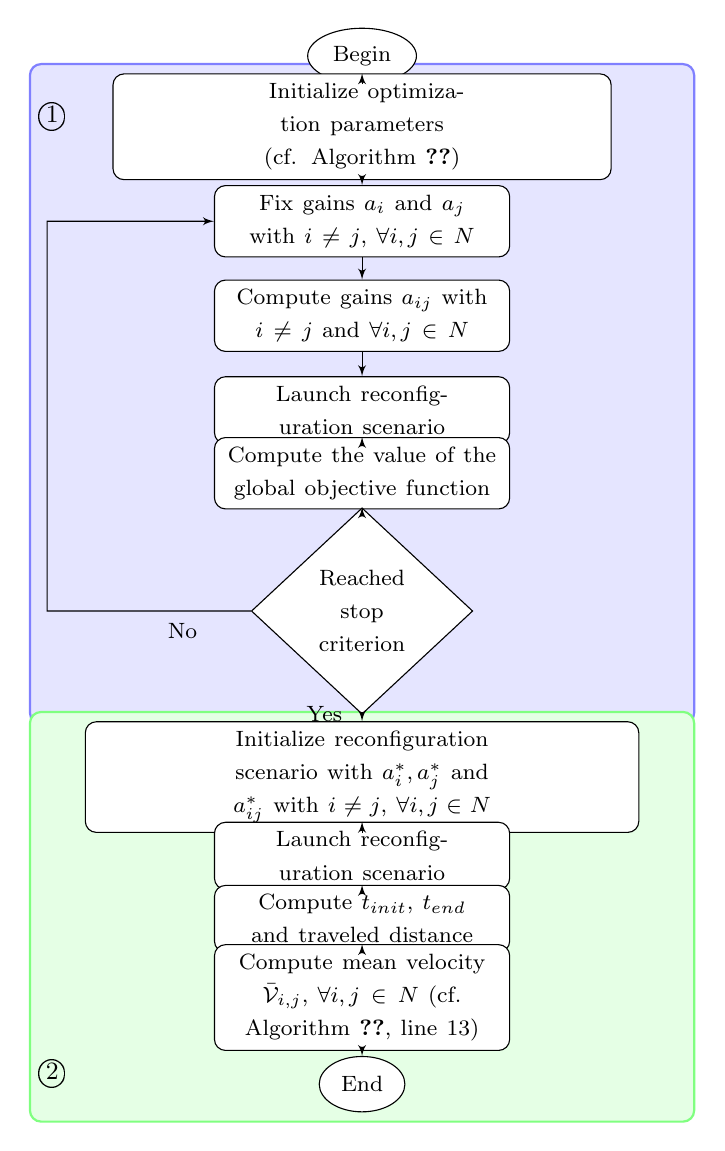
\begin{tikzpicture}[scale=2, node distance = 1.2cm, auto]
    % Place nodes
    \tikzstyle{bigbox} = [minimum width=24em,draw=blue!50, thick, fill=blue!10, rounded corners, rectangle]
    \tikzstyle{bigbox2} = [minimum width=24em,draw=green!50, thick, fill=green!10, rounded corners, rectangle]

    \node [cloud] (n1) {\footnotesize Begin}; 
    \node [block, below of= n1,minimum height=1em,  minimum width=18em ,node distance= 0.9cm] (n2){\footnotesize{ Initialize optimization  parameters (cf. Algorithm \ref{alg: optimization algorithm})}};
    \node[block, below of= n2, minimum height=1em, minimum width=10em](n3){\footnotesize Fix gains $a_{i}$ and $a_j$ with $i \neq j $, $\forall i,j\in {N}$}; 
    \node[block, below of= n3, minimum height=1em, minimum width=10em](n4){\footnotesize Compute gains $a_{ij}$  with $i\neq j$ and $\forall i,j\in {N}$}; 
    \node[block, below of= n4, minimum height=1em, minimum width=10em](n5){\footnotesize Launch reconfiguration scenario}; 
    \node[block, below of= n5, minimum height=1em, minimum width=10em,node distance= 0.8cm](n6){\footnotesize Compute the value of the global objective function};
    \node[decision, below of= n6,minimum height=1em, minimum width=8em,node distance= 1.75cm ] (n7) {\footnotesize Reached stop criterion}; 
    \node[block, below of= n7, minimum height=1em, minimum width=20em,node distance= 6em](n8){\footnotesize Initialize reconfiguration scenario with $a_i^*,a_j^*$ and $a_{ij}^* $ with $i \neq j $, $\forall i,j\in {N}$}; 
    \node[block, below of= n8,minimum height=1em, minimum width=10em, node distance= 1cm](n9){\footnotesize Launch reconfiguration scenario}; 
    \node[block, below of= n9, minimum height=1em, minimum width=10em,node distance= 0.8cm](n10){\footnotesize Compute $t_{init}$, $t_{end}$ and traveled distance};         
    \node[block, below of= n10, minimum height=1em, minimum width=10em,node distance= 1cm](n11){\footnotesize Compute mean velocity $\bar{\mathcal{V}}_{i,j}$, $\forall i,j \in  {N}$ (cf. Algorithm \ref{alg: projection and computation of the mean velocity }, line 13)}; 
    \node[cloud, below of= n11,node distance= 1.1cm] (n12){\footnotesize End};  

    % Draw edges 
    \path[line] (n1)--(n2)node[text width=23.5em,text height=0em]{ \textcircled{\small{1}}}; 
    \path[line] (n2)--(n3); 
    \path[line] (n3)--(n4); 
    \path[line] (n4)--(n5); 
    \path[line] (n5)--(n6); 
    \path[line] (n6)--(n7); 
    \path[line] (n7.west) node [text width=6em,text height=2em]{\footnotesize No} -|(-2,-1.05)   -- (n3.west) ;
    \path[line] (n7)node [text width=4em,text height=8em]{\footnotesize Yes}--(n8); 
    \path[line] (n8)--(n9); 
    \path[line] (n9)--(n10); 
    \path[line] (n10)--(n11); 
    \path[line] (n11)--(n12) node [text width=23.5em,text height=-10em]{ \textcircled{\small{2}}}; 
    \begin{pgfonlayer}{background}
    \node[bigbox] [fit = (n2) (n7)] {};
    \node[bigbox2] [fit = (n8) (n12)] {};

   \end{pgfonlayer}
\end{tikzpicture}
\end{center}
%\vspace{-4mm}
\caption{The proposed CORM (Constrained Optimal Reconfiguration Matrix) flowchart. \numcircledmod{1} The optimization algorithm. \numcircledmod{2} The projection and mean velocity computation}
\label{fig:CormAlgo}
%\vspace{-5mm}%Put here to reduce too much white space after your table 

\end{figure} 
















In Figure \ref{fig:CormAlgo}, the details of the optimization process are illustrated. Following eq. \ref{eq:costfunction}, through the optimization algorithm based on gradient descent, it is aimed to compute the diagonal gains of the reconfiguration matrix $A$. The objective function is non-linear, the optimization algorithm (cf. Algorithm \ref{alg: optimization algorithm}, inputs) needs the optimization boundaries $[{a}_{i,j_{min}}, {a}_{i,j_{max}}]^T$  and the starting point $[a_{i_0}, a_{j_0}]^T$ with $i \neq j $, $\forall i,j\in {N}$. The anti-diagonal gains of $A$, in charge of the inter-target distances, are computed while using eq. \ref{eq:FinalDistaneStudy_2}. 

The full merging scenario is launched with a constant reconfiguration matrix $A$. The data related to the merging scenario are used to compute the objective function in eq. \ref{eq:costfunction} (cf. Algorithm \ref{alg: optimization algorithm}). The latter is used to judge on the stop criterion; when the minimum of the cost function is reached. At last, the optimization algorithm returns the optimal values of the gains $a_i^*$ and $a_j^*$, $i \neq j $, $\forall i,j\in {N}$, the gains $a_{ij}, i\neq j,  i,j\in {N}$ are computed with the help of eq. \ref{eq:FinalDistaneStudy_2}.




\begin{algorithm}
\begin{small}
\DontPrintSemicolon
\SetKwInOut{Input}{Input}
\SetKwInOut{Output}{Output}
\SetKwInOut{Variables}{Variables}
\SetKwInOut{Parameters}{Parameters}
\Input{$GlobalInput$  Scenario data \\$[{a}_{i_{min}}, {a}_{i_{max}}]^T$ boundaries of the gain $a_i$ \\
$[{a}_{j_{min}}, {a}_{j_{max}}]^T$ boundaries of the gain $a_j$ \\ $[{a_{i_{0}}}, {a_{j_{0}}}]^T$start point of the optimization \\
$ObjectiveFunction$ the objective function in eq. \ref{eq:costfunction}}% an intervention}


\Output{$[a_i^*,a_j^*]^T $ optimal values of the gains $a_i$ and $a_j$ } 
$MergingData \leftarrow [PerpDist\{T_{d_{i}}, {T}_{p_{i}}\},PerpDist\{T_{d_{j}}, {T}_{p_j}\},$
$ PerpDist\{{T}_{p_i}, Border\}, PerpDist\{{T}_{p_j}, Border\}]^T $\;
\While{$(StopCriterion \neq True)$}
{
  %\tcp*[l]{next intervention of ordered list of interventions to be scheduled }
  $[a_{i}, a_{j}]^T \leftarrow Fixe([{a_{i_{0}}}, {a_{j_{0}}}]^T, [{a}_{i}_{min}, {a}_{i}_{max}]^T,[{a}_{j}_{min}, {a}_{j}_{max}]^T )$\; 
   $MergingData \leftarrow MergingScenario(GlobalInput, a_i, a_j) $\; 
  %\tcp*[l]{select modes and time intervals for intervention $p$}
  %\tcp*[l]{assess cost}
  $T \leftarrow length(MergingData)$ \;
  \ForAll{$t \in [0, T]$}
  {
    $Cost(t) \leftarrow ObjectiveFunction(MergingData(t)) $
  }
  $GlobalCost \leftarrow Sum(Cost)$
  
}
%\Return $S_i, \mathcal{L}_{u}$\;
\caption{Optimization Algorithm}\label{alg: optimization algorithm}
\end{small}

\end{algorithm}


\subsubsection{Safe and feasible local trajectory planning}  \label{sec:Projected_target}

In this section it is proposed to delve into the projection approach based on a Frenet reference frame that ensures the respect of the global reference path imposed by the global reference planner. In addition, this section presents the computation of the velocity profile imposed to the projected target $T_p$ to ensure the safety, feasibility, and smoothness of the merging maneuver. 

\begin{enumerate}
    \item \textbf{\textit{Global reference aware target:}} The constrained optimal inter-target distance matrix allows to respect the road constraints while ensuring the vehicle's safety. However, the generated targets $T_d$ are not guaranteed to be onto the reference path (cf. Figure \ref{fig:CORM-approximation} \numcircledmod{1}). In order to ensure this requirement, it is proposed to use the reference path as a guiding system for the vehicle and compute its effective target $T_p$ w.r.t. this latter (cf. Figure \ref{fig:CORM-approximation} \numcircledmod{1}).

    Each target $T_d$ of the merging vehicle is projected w.r.t. the reference merging path using a Frenet reference frame $[X_f,Y_f]$ (cf. Figure \ref{fig:CORM-approximation}) to obtain $T_p$. The lines 10 and 11 in Algorithm \ref{alg: projection and computation of the mean velocity } and eq. \ref{eq:frenetToCartisian} details the transformation from the mobile reference frame centered on $V_R$ to the global reference frame $[X_G,Y_G]$, in addition to the projection function that uses the reference merging path and $T_d \in \mathcal{M}$ to obtain $T_p$ (cf. Figure \ref{fig:CORM-approximation} \numcircledmod{1})


    \item \textbf{\textit{Safe and feasible velocity profile:}} The projected target $T_p$ has a similar dynamic as $T_d$. However, in order to draw full advantage from the constrained optimal inter-target distance matrix in terms of safety formal insurance, it is proposed to use the latter to compute the necessary mean velocity that must be imposed to the vehicles, such that they enter the conflicting zone in Figure \ref{fig:CORM-approximation} \numcircledmod{2} at the same moment as if they have followed $T_d$. 

    Before the presentation of the details related to the imposed dynamics, for the clarity and the understanding of the reader, it is proposed to define the conflicting zone. The conflicting zone in  Figure \ref{fig:CORM-approximation} \numcircledmod{2} defines the area where a collision between the merging vehicle and the vehicle on the highway vehicle may occur. $\mathcal{P}_{merging}$ defines the position of the merging vehicle where the surrounding circles of $V_i$ and $V_j$ may overlap, resulting in a collision. The points $A$, $B$, $C$, and $D$ define the limits of the conflicting zone. $A$ is the pose of the merging vehicle where a collision may occur, $B$ is related to the limits of the merging zone, $D$ defines the end of the merging zone, while $C$ is its projection w.r.t. the highway center-line (cf. Figure \ref{fig:CORM-approximation} \numcircledmod{2}). 


\begin{algorithm}
\begin{small}
\DontPrintSemicolon
\SetKwInOut{Input}{Input}
\SetKwInOut{Output}{Output}
\SetKwInOut{Variables}{Variables}
\SetKwInOut{Parameters}{Parameters}
\Input{$GlobalInput$  Scenario data \\  $a_i^* , a_j^*, a_{ij}^*$ optimal gains of the reconfiguration matrix (cf. Algorithm \ref{alg: optimization algorithm})} % an intervention}


\Output{$\widebar{\mathcal V}_{i,j}$ the mean velocity of the vehicles $V_i$ and $V_j$}

%\Variables{$\mathcal{S}_{p,sr(ti)c}$ for intervention $p$, \\
%\hspace{35pt} set of quadruplets (\textbf{s}urgeon, \textbf{r}oom, 
%\textbf{t}ime \textbf{i}nterval, \textbf{c}ost)}
%\vspace{5pt}
%$\mathcal{L}_{u} \leftarrow \emptyset$ \;
$k \leftarrow 1$ \; 
$\mathcal{F}(k) \leftarrow {F^{init}}$\; 
$\varepsilon (k) \leftarrow  \mathcal{F}^{end}-\mathcal{F}(k)$\; 
$ Buffer_R \leftarrow ReferenceTrajectory(V_R)$\;
$ Buffer_{i,j} \leftarrow ReferenceTrajectory(V_i,V_j)$\;

\While{$(\varepsilon (k)\neq 0)$}
{
  $k \leftarrow k+1$ \; 
  %\tcp*[l]{next intervention of ordered list of interventions to be scheduled }
  $\mathcal{F} (k) \leftarrow DynamicReconfiguration ( \mathcal{F}^{end},\mathcal{F}(k-1)) $\;
  $\varepsilon (k) \leftarrow  \mathcal{F}^{end}-\mathcal{F}(k)$\; 
  %\tcp*[l]{select modes and time intervals for intervention $p$}
  %\tcp*[l]{assess cost}
  $T_{d_{i,j}}(k) \leftarrow Transform(Buffer_R,\mathcal{F}(k), X_{V_{R}})  $ \;
  ${T}_{p_{i,j}}(k) \leftarrow Projection(Buffer_{i,j},{T}_{d_{i,j}})  $ \;
  $X_{V_{i,j}} (k)  \leftarrow Control(X_{V_{i,j}} (k-1),{T}_{p_{i,j}}(k))$\; 
  }
  $\widebar{\mathcal V}_{i,j}= \frac{CurviDist \{V_{i,j}(1,k)\}}{t_{end}-t_{init}}$\;
 
%\Return $S_i, \mathcal{L}_{u}$\;
\caption{\small Projections and computation of the imposed dynamic \label{alg: projection and computation of the mean velocity }}
\end{small}
\end{algorithm}




    Based on the definition of the conflicting zone, it is proposed to compute the mean velocity $\bar{\mathcal{V}}_{i,j}$ where $i,j$ are the indices of the vehicles $V_i$ and $V_j$ respectively (cf. Figure \ref{fig:CORM-approximation} \numcircledmod{2}), such that the in-between distance respects the following:  
\begin{align}
    EucDist \{\bar{T}_{p_j}(t_{end}),\bar{T}_{p_i}(t_{end})\}= 
    EucDist \{T_{d_j}(t_{end}),T_{d_i}(t_{end})\}
\end{align}

where $t_{end}$ is the time when the pose $\mathcal{P}_{merging}$ (cf. Figure \ref{fig:CORM-approximation}) is reached by the merging vehicle. $EucDist \{T_{d_j}(t_{end}),{T}_{d_i}(t_{end})\}$  represents the Euclidean distance between the targets $T_{d_{i}}$ and $T_{d_j}$ generated during the first step of the proposed CORM for the vehicles $V_i$ and $V_j$, while $EucDist \{\bar{T}_{p_j}(t_{end}),\bar{T}_{p_i}(t_{end})\}$ (Figure \ref{fig:CORM-approximation} \numcircledmod{2}) is the in-between Euclidean distance between the targets with the imposed dynamic $\bar{\mathcal{V}}_{i}$  and  $\bar{\mathcal{V}}_{j}$ for the vehicles $V_i$ and $V_j$, respectively.  



The mean velocity $\bar{\mathcal{V}}_{i,j}$ where $i,j$ are the indices of the vehicles $V_i$ and $V_j$ (Figure \ref{fig:CORM-approximation} \numcircledmod{2}) is computed based on the line 13 in Algorithm \ref{alg: projection and computation of the mean velocity }, where $t_{init}$ is the corresponding time when the reconfiguration was launched. A curvilinear distance formula is used to get the traveled distance by each vehicle between $t_{init}$ and $t_{end}$. 




In order to have the smoothest possible behavior w.r.t. the vehicles' dynamics, it is proposed to use a sigmoid function to shape the velocity profile. This latter is used to create a velocity profile that goes from the vehicle initial velocity toward the mean velocity, and goes to the reference vehicle $V_R$ velocity when the vehicle enters the main line. This choice is motivated by the sigmoid ability to smoothly control the convergence rate from an initial velocity to the final desired one. In other terms, using the sigmoid function permits us to impose a feasible and comfortable acceleration and deceleration profile to the vehicles. 








    
\end{enumerate}


\subsection{Simulation results}\label{sec:CORM_simulation}

In order to evaluate the efficiency of the CORM in terms of its ability to guarantee the safety requirement as well as the smoothness of the vehicle's dynamics, while performing the on-ramp merging maneuver, a first scenario is proposed. It aims to perform the merging maneuver with a formation of three vehicles. The simulation video can be found in \textcolor{blue}{https://youtu.be/UM2cLt74pVM}. Then, a comprehensive summary of several conducted simulations is presented in Table \ref{Tab: Summary}. 

\begin{enumerate}
    \item \textbf{\textit{On-ramp merging in formation:}} 
    
        \begin{figure}[!h]
        \centering 
        \includegraphics[width=14cm,height=18cm,keepaspectratio]{chapters/Chapitre_5/Figures/CORM/MergingSimulation.pdf}
        %\vspace{-2.3mm}
        \caption{Evolution of the formation shape during the merging performed by the CORM framework (\textcolor{blue}{Simulation video: https://youtu.be/UM2cLt74pVM})}
        \label{fig:CORM: formation_shape}
        %\vspace{-5mm}
        \end{figure}

    In the following simulation, it is aimed to perform a merging maneuver with a formation of three vehicles. The considered merging scenario is an on-ramp merging with an incidence angle $\mu=10^\circ $, $V_1$ (i.e., the reference vehicle $V_R$) is placed in the main line, so as $V_2$. The third vehicle $V_3$ initially placed in the secondary on-ramp merging road (cf. Figure \ref{fig:CORM: formation_shape}). The initial formation shape is triangular (cf. Figure \ref{fig:CORM: formation_shape}), consequently at the end of the reconfiguration phase the aim is to put the vehicles part of the formation in a linear shape to form a platoon (cf. Figure \ref{fig:CORM: formation_shape}). Table \ref{Tab: inputs} resumes the scenario inputs. 

\begin{table}[]
%\scriptsize
\begin{center}
\caption{The values of the inputs of the CORM algorithm}

\label{Tab: inputs}

\begin{tabular}{lll}

\cline{1-2}  
\multicolumn{1}{|l|}{Inputs}                                    & \multicolumn{1}{l|}{Values}                                                                                                                              &  \\ \cline{1-2}                 
\multicolumn{1}{|l|}{Initial formation coordinates $[m]$}       & \multicolumn{1}{l|}{\begin{tabular}[c]{@{}l@{}}$\left (\begin{smallmatrix}\\   0 & -40 &-50 \\\\   0 &0& 9.2 \\  \end{smallmatrix}\right)$\end{tabular}} &  \\ \cline{1-2}
\multicolumn{1}{|l|}{Final formation coordinates $[m]$} & \multicolumn{1}{l|}{\begin{tabular}[c]{@{}l@{}}$\left(\begin{smallmatrix}\\ 0 &-80&-40\\\\ 0&0&0\\ \end{smallmatrix}\right)$\end{tabular}}                                    &  \\ \cline{1-2}
\multicolumn{1}{|l|}{$\mathcal{V}_{1,2,3}[m/s]$}                & \multicolumn{1}{l|}{$[19.4, 19.4,19.4]$}                                                                                                              &  \\ \cline{1-2}
\multicolumn{1}{|l|}{$[{a}_2_{min}, {a}_2_{max}]^T$}     & \multicolumn{1}{l|}{$[-0.4, 0.1]$}                                                                                                                     &  \\ \cline{1-2}
\multicolumn{1}{|l|}{$[{a}_3_{min}, {a}_3_{max}]^T$}     & \multicolumn{1}{l|}{$[-0.4, -0.05]$}                                                                                                                   &  \\ \cline{1-2}
\multicolumn{1}{|l|}{$[a_{2_{0}}, a_{3_{0}}]^T$}                & \multicolumn{1}{l|}{$[-0.25, -0.25]$}                                                                                                                  &  \\ \cline{1-2}
\multicolumn{1}{|l|}{$[w_2, w_3]^T$}                  & \multicolumn{1}{l|}{$[1, 4]$}                                                                                                                          &  \\ \cline{1-2}
\multicolumn{1}{|l|}{$[a_{2}^*, a_{3}^*]^T$}                    & \multicolumn{1}{l|}{$[-0.1228, -0.365]$}                                                                                                               &  \\ \cline{1-2}
\multicolumn{1}{|l|}{$\underline{D}_T[m]$}                      & \multicolumn{1}{l|}{$12$}                                                                                                                                &  \\ \cline{1-2}
                                                                &                                                                                                                                                          & 
\end{tabular}
\end{center}
\vspace{-10mm}%Put here to reduce too much white space after your table 
\end{table}


    

    The minimum inter-target distance $\underline{D}_T$ (cf. Figure \ref{fig:safetydistance}) is computed using the following model: 
    \begin{equation} \label{eq:minimum_distance_model}
    \underline{D}_T= (R_i + R_j)  + offset
    \end{equation}

    where $R_i$ and $R_j$ are the radius of the circles that surround the vehicles $V_i$ and $V_j$, and $offset$ is the safety distance to avoid rear-end collisions. 











The reconfiguration of the triangular shape toward the desired linear one is illustrated in Figure \ref{fig:CORM: formation_shape}. The formation defined by its initial coordinates passes through the reconfiguration phase, where $V_3$ is in front of $V_2$ as desired w.r.t. the formation's final coordinates, consequently, the $EucDist(V_1,V_2)$ needs to increase. The intermediate formation showcases the pose of the three vehicles in the conflict zone. As expected $EucDist(V_1,V_2)$ has increased to make space for $V_3$ in the convoy. In the second phase, after the convergence of the formation toward its desired shape, the vehicles form a linear shape, where the desired in-between distances are respected. 

        \begin{figure}[!h]
        \centering 
        \includegraphics[width=11cm,height=18cm,keepaspectratio]{chapters/Chapitre_5/Figures/CORM/In_between_distances.pdf}
        %\vspace{-2.3mm}
        \caption{The formation coordinates and the Euclidean in-between distances profiles}
        \label{fig:CORM: formation_coordinates}
        %\vspace{-5mm}
        \end{figure}

To evaluate the CORM capability in terms of safety and convergence errors, it is proposed to study the evolution of the formation coordinates and the in-between distances profiles illustrated in Figure \ref{fig:CORM: formation_coordinates}. A first order asymptotic convergence from the initial formation shape toward the desired one can be noticed in the formation coordinates plots. As for the minimum distances, the in-between distances profiles are always greater than $\underline{D}_T$. The in-between distances when the vehicles are in the conflicting zone is greater than  $20m$. The final in-between distances meet the safety requirement for a convoy formation; $EucDist(V_i, V_j)=2[s]\times \mathcal{V}_{i,j}[m/s]=40m$. 


        \begin{figure}[!h]
        \centering 
        \includegraphics[width=10cm,height=18cm,keepaspectratio]{chapters/Chapitre_5/Figures/CORM/velocities.pdf}
        %\vspace{-2.3mm}
        \caption{The vehicles' velocity and acceleration profiles}
        \label{fig:CORM: velocity}
        %\vspace{-5mm}
        \end{figure}





In Figure \ref{fig:CORM: velocity}, the linear velocity, the longitudinal, and the lateral accelerations are presented for each of the three vehicles part of the formation. As expected, the velocity of the vehicle $V_2$ decreases at the beginning of the scenario to make space for $V_3$, before it increases to make sure that $V_2$ meets the velocity requirement in the platoon. As for $V_3$, its velocity increases at the beginning to enter the highway center-line while respecting the safety distances. A decreasing can be noticed around $4s$ to follow the convoy velocity (fixed to $19.4 m/s$ - $70 km/h$). Figure \ref{fig:CORM: velocity} confirms that the longitudinal and the lateral accelerations respect the maximum and minimum authorized accelerations (i.e., $-4m/s^2$ for deceleration and $3m/s^2$ for acceleration). Thus, with the help of the results in Figure \ref{fig:CORM: velocity}, the vehicles' dynamics during the formation reconfiguration while the merging is performed are smooth and comfortable. 




 \item \textbf{\textit{Influence of the projection phase on the CORM efficiency:}} 

 This section is dedicated to validate more intensively the proposed approach, while emphasizing mainly the ability of the projection phase for different environments structure (several values of $\mu$). 

        % \begin{figure}[!h]
        % \centering 
        % \includegraphics[width=10cm,height=18cm,keepaspectratio]{chapters/Chapitre_5/Figures/CORM/CORM_summary.pdf}
        % %\vspace{-2.3mm}
        % \caption{Range of incidence angles between $ \mu = 10^\circ$ and $\mu = 30^\circ$}
        % \label{fig:CORM: mu}
        % %\vspace{-5mm}
        % \end{figure}

 

For a range of incidence angles between $ \mu = 10^\circ$ and $\mu = 30^\circ$ with $\Delta \mu = 10^\circ$ step each time. It is proposed to study the performance of the CORM for velocity between $5 m/s$ and $15 m/s$ with an increase of $5 m/s$ each time. For all the simulations, the inputs of the CORM algorithm are the same as in Table \ref{Tab: inputs}. The conducted simulations are summarized in Table \ref{Tab: Summary}.



According to the performed simulations, it is important to emphasize that the safety of the vehicles is always ensured; the minimum inter-vehicle distance in the conflicting zone $\underline{D_{T}}$  is always greater than $20m$. The metric $Error_{max}$ is the maximum distance between $T_d$ and $\bar{T}_{p}$. This latter is lower than $1.5m$ (distance between the center-line and the road border), in other terms, $T_d$ is never out of the road borders. 

To evaluate the smoothness of the merging, it is proposed to discuss the obtained velocity and acceleration profiles w.r.t. variable velocity of the reference velocity and different incidence angles. The velocity profiles are similar to the one in Figure \ref{fig:CORM: velocity}, with a sigmoid shape that makes $\mathcal{V}_2$ decrease toward $\underline{\mathcal{V}}_2$ to make space for $V_3$, and $\mathcal{V}_3$ increase toward $\bar{\mathcal{V}}_3$ in the beginning. Then, $\mathcal{V}_2$ and $\mathcal{V}_3$ increases and decreases respectively toward $\mathcal{V}_R$ to form the final desired platoon. As for the acceleration, the lateral and the longitudinal behavior respect the limits of feasibility and comfort (i.e., $-4 m/s^2$ for the deceleration and $3m/s^2$ for the acceleration).
 



\newpage
\thispagestyle{empty}
\begin{landscape}
\begin{table*}[!h]
\setlength\tabcolsep{6.5pt} % default value: 6pt
%\scriptsize

\centering
\caption{The summary results of the conducted simulation for a variable incidence angle $\mu$ and vehicles' velocity $\mathcal{V}$ }
  %\centering
  %\captionsetup{singlelinecheck=off, skip =4pt}
  \begin{adjustwidth}{-0.235\textwidth}{-0.10\textwidth}
%\vspace{-2.3mm}
\label{Tab: Summary}

\begin{tabular}{|l|lll|lll|lll|}
\hline
$\mu[\deg]$                                                       & \multicolumn{3}{l|}{10}                                                                                            & \multicolumn{3}{l|}{20}                                                                                          & \multicolumn{3}{l|}{30}                                                                                     \\ \hline
$\mathcal{V}_{R}[m/s]$                                            & \multicolumn{1}{l|}{5}                     & \multicolumn{1}{l|}{10}                    & 15                       & \multicolumn{1}{l|}{5}                   & \multicolumn{1}{l|}{10}                    & 15                       & \multicolumn{1}{l|}{5}                    & \multicolumn{1}{l|}{10}                  & 15                   \\ \hline
$[\underline{\mathcal{V}}_{2}, \overline{\mathcal{V}}_{2}][m/s]$  & \multicolumn{1}{l|}{{[}4.36, 5{]}}       & \multicolumn{1}{l|}{{[}8.73,10{]}}      & {[}13.45, 15{]}        & \multicolumn{1}{l|}{{[}4.21, 5{]}}     & \multicolumn{1}{l|}{{[}8.49,10{]}}       & {[}13.26, 15{]}        & \multicolumn{1}{l|}{{[}4.13, 5{]}}      & \multicolumn{1}{l|}{{[}8.35,10{]}}     & {[}13.06,15{]}     \\ \hline
$[\underline{\mathcal{V}}_{3}, \overline{\mathcal{V}}_{3}][m/s]$ & \multicolumn{1}{l|}{{[}5,5.59{]}}       & \multicolumn{1}{l|}{{[}10,11.125{]}}      & {[}15,16.80{]}         & \multicolumn{1}{l|}{{[}5,5.824{]}}       & \multicolumn{1}{l|}{{[}10,11.6316{]}}      & {[}15,17.43{]}           & \multicolumn{1}{l|}{{[}5,6.10{]}}       & \multicolumn{1}{l|}{{[}10,12.10{]}}    & {[}15,18.14{]}     \\ \hline
$[\underline{a}_2,\overline{a}_2]_{long}[m/s^2]$                  & \multicolumn{1}{l|}{{[}-0.29, 0.15{]}} & \multicolumn{1}{l|}{{[}-0.60, 0.29{]}} & {[}-0.70, 0.35{]}{]} & \multicolumn{1}{l|}{{[}-0.35, 0.18{]}}  & \multicolumn{1}{l|}{{[}-0.68, 0.34{]}} & {[}-0.78, 0.53{]} & \multicolumn{1}{l|}{{[}-0.38,0.19{]}} & \multicolumn{1}{l|}{{[}0.70,0.37{]}}  & {[}-0.87,0.44{]} \\ \hline
$[\underline{a}_2,\overline{a}_2]_{lat}[m/s^2]$                   & \multicolumn{1}{l|}{{[}0,0{]}}             & \multicolumn{1}{l|}{{[}0,0{]}}             & {[}0,0{]}                & \multicolumn{1}{l|}{{[}0,0{]}}           & \multicolumn{1}{l|}{{[}0,0{]}}             & {[}0,0{]}                & \multicolumn{1}{l|}{{[}0,0{]}}            & \multicolumn{1}{l|}{{[}0,0{]}}           & {[}0,0{]}            \\ \hline
$[\underline{a}_3,\overline{a}_3]_{long}[m/s^2]$                  & \multicolumn{1}{l|}{{[}-0.76,1.52{]}}  & \multicolumn{1}{l|}{{[}-1.66, 2.02{]}}    & {[}-1.14,2.27{]}      & \multicolumn{1}{l|}{{[}-0.570,1.07{]}}  & \multicolumn{1}{l|}{{[}-1.66, 2.02{]}}    & {[}-1.54,2.92{]}     & \multicolumn{1}{l|}{{[}-0.65,1.39{]}} & \multicolumn{1}{l|}{{[}-1.31,2.55{]}} & {[}-2.00,2.75{]} \\ \hline
$[\underline{a}_3,\overline{a}_3]_{lat}[m/s^2]$                   & \multicolumn{1}{l|}{{[}-0.29,0.74{]}}  & \multicolumn{1}{l|}{{[}-0.39,0.80{]}}  & {[}-0,74,1.38{]}     & \multicolumn{1}{l|}{{[}-0.84,0.75{]}} & \multicolumn{1}{l|}{{[}-1.02,0.96{]}}  & {[}-1.60,1.59{]}       & \multicolumn{1}{l|}{{[}-1.56,1.55{]}}  & \multicolumn{1}{l|}{{[}-2.23,1.94{]}} & {[}-3.63,2.53{]} \\ \hline
$\underline{D}[m]$                                                & \multicolumn{1}{l|}{21.66}               & \multicolumn{1}{l|}{21.80}               & 23.30                  & \multicolumn{1}{l|}{24.75}               & \multicolumn{1}{l|}{24.01}                 & 23.30                  & \multicolumn{1}{l|}{28.70}                & \multicolumn{1}{l|}{27.30}             & 25.725               \\ \hline
{\ul ${Error}_{max}[m]$}                                               & \multicolumn{1}{l|}{{ 0.52}}          & \multicolumn{1}{l|}{0.73}                & { 0.78}             & \multicolumn{1}{l|}{{ 0.85}}        & \multicolumn{1}{l|}{{ 0.88}}          & 0.92                   & \multicolumn{1}{l|}{1.10}               & \multicolumn{1}{l|}{1.13}              & 1.14               \\ \hline
\end{tabular}
\end{adjustwidth}
\end{table*}
\end{landscape}









    
\end{enumerate}






\subsection{Conclusion on the CORM algorithm}\label{sec:CORM_conclusion}
This section extensively explored the topic of cooperative formation reconfiguration, with the help of the proposed Constrained Optimal Reconfiguration Matrix (CORM) framework. The CORM framework can be succinctly described as a two-step process: 

\begin{enumerate}
    \item First, it employs an optimization algorithm that explicitly accounts for environmental constraint. This step focuses on the computation of the convergence rate necessary for the constrained inter-target distance matrix $A$. This matrix is responsible for reshaping the virtual structure from its initial configuration to the desired shape required for executing the on-ramp merging maneuver. 

    \item The second step is based on a projection approach with safe and appropriate dynamics. It ensures that each vehicle within the formation, participating in the merging scenario, effectively tracks the dynamic target while aligning with the global reference frame. In this step, the targets determined in step (1) are projected onto a Frenet reference frame linked to the global reference path. This ensures alignment with the global path and a smooth velocity profile is generated using a sigmoid shape, guaranteeing a smooth merging maneuver. 
\end{enumerate}


The evaluation of the CORM algorithm was carried out in a simulation environment. It showcased the algorithm's ability to adhere to safety criterion, even in challenging scenarios involving high-speed merging. The algorithm's suitability for varying incidence angles $\mu$ of the merging road and diverse formation dynamics was demonstrated through extensive simulations.


However, it is crucial to acknowledge the limitations of the CORM algorithm. One of its key limitations is that it assumes the same dynamics for both longitudinal and lateral reconfiguration. In other words, it employs identical control gains for both longitudinal and lateral coordinates reconfiguration during the merging. Additionally, the generated trajectory with the constrained inter-target distance matrix does not seamlessly align with the imposed reference trajectory, particularly when reconfiguring the position of the merging vehicle from a secondary road location to the highway center-line.

Taking these limitations into account and in the optic of mitigating them, the following section presents the Extended Dynamic Reconfiguration Matrix (E-CORM). 






%For instance, the nearest highway vehicle w.r.t. merging zone is considered as the reference vehicle (cf. Figure \ref{} \textcolor{red}{ajouter une figure qui montre l'identification des véhicules par la RSU}). 

%The proposed formation modeling approach relies on the virtual structure approach (cf. Section \textcolor{red}{ajouter la ref de la virtual structure}), thus the reference vehicle plays a pivotal role in the formation modeling. In facts, the virtual structure approach relies on a reference frame to compute the coordinates of the agents part of the formation 





%As stated in Chapter \textcolor{red}{ajouter le chapitre sur }, the objective of the group of $N$ vehicles part of the MVS is to reach and keep their assigned configuration w.r.t. to the desired formation shape and the reference vehicle configuration. 

\newpage
\section{Extended Dynamic Reconfiguration Matrix (E-CORM)} \label{sec:E-CORM}
As stated in Section \ref{sec:CORM_conclusion}, the proposed CORM framework uses a restricted motion convergence approach which limits its flexibility. Taking this limitation into account, the Extended Constrained Optimal Reconfiguration Matrix (E-CORM) proposes to decorrelate the dynamic of the longitudinal and the lateral coordinates, allowing more flexibility; in addition to a road segmentation approach that permits to respect the global path imposed by the global trajectory planning level. 

Before the presentation of the details of the proposed E-CORM for formation reconfiguration, and for the clarity of this PhD manuscript and the understanding of the reader, it is important to note that the formation definition and configuration formalism used for the E-CORM is the same as the one used for the CORM (cf. Section \ref{sec:formation_modeling_section}). 

The following section is dedicated to the presentation of the details of the proposed E-CORM. Thus, in Section \ref{se:E-CORM_formalisme}, the extended inter-target distance matrix is presented. Section \ref{sec:RoadSegmentationStrategie} details the toad segmentation approach used part of the E-CORM. In Section \ref{sec:Simulation_E-CORM}, the simulations results related to the E-CORM performance are discussed. Lastly, Section \ref{sec:Conclusion_E-CORM} concludes on E-CORM's advantages and limitations. 




\subsection{Extended inter-target distance matrix} \label{se:E-CORM_formalisme}
In order to characterize the evolution of the reconfiguration from the initial shape toward the desired one, while ensuring the respect of the safe inter-target distance $\underline{D}_T$ between the $N$ vehicles part of the formation, the E-CORM proposes an intermediate state vector $S$ given as the following: 
\begin{equation} \label{eq:BasicInitialEquation}
    S = \dot{e} + \lambda e  + \gamma \smallint e\; dt\\
\end{equation}

To overcome the CORM lack of flexibility, the E-CORM uses in addition to the convergence error $e$ (cf. eq. \ref{eq: errorbetweenfinitandfendforvi}), the convergence rate $\dot{e}$ of the error and the sum of the errors through the integrative term of the latter. $\lambda, \; \gamma  \in \mathbb{R}^+ $ are the convergence gains and permit to offer more flexibility to the E-CORM algorithm. 

The convergence of $S$ follows a first order convergence model detailed in eq. \ref{eq:BasicInitialEquation_ECORM}. 

\begin{equation} \label{eq:BasicInitialEquation_ECORM}
    \dot{S} = A \times S = A \dot{e} +  A \lambda e  + A \gamma \smallint e\; dt \\
\end{equation}
where $A^{2N\times 2N}$ is a negative-definite convergence matrix.


Using eq. (\ref{eq: errorbetweenfinitandfendforvi}}) in eq. (\ref{eq:BasicInitialEquation_ECORM}) permits to write the extended system of equations representing the studied system. 


\begin{eqnarray} \label{eq:SystemOfBasicEquation_E-CORM}
  \dot{S}_{h_{1}} &=& a_{h_{1}}\dot{e}_{h_{1}} + a_{h_{1}}\lambda_{h_{1}}e_{h_{1}}+a_{h_{1}}\gamma_{h_{1}} \smallint e_{h_{1}}dt\\ \nonumber
  \dot{S}_{l_{1}} &=& a_{l_{1}}\dot{e}_{l_{1}} + a_{l_{1}}\lambda_{l_{1}}e_{l_{1}}+a_{l_{1}}\gamma_{l_{1}} \smallint  e_{l_{1}}dt\\ \nonumber
        &\vdots& \\ \nonumber
  \dot{S}_{h_{N}} &=& a_{h_{N}}\dot{e}_{h_{N}} + a_{h_{N}}\lambda_{h_{N}}e_{h_{N}}+a_{h_{N}}\gamma_{h_{N}} \smallint  e_{h_{N}}dt\\ \nonumber
  \dot{S}_{l_{N}} &=& a_{l_{N}}\dot{e}_{l_{N}} + a_{l_{N}}\lambda_{l_{N}}e_{l_{N}}+a_{l_{N}}\gamma_{l_{N}} \smallint e_{l_{N}}dt\\ \nonumber
\end{eqnarray}

\noindent where $h_i$ and $l_i$, representing the longitudinal and the lateral coordinates of the formation, converge toward the target with different convergence rates $a_{h_i}$ and $a_{l_i}$. 


The system in eq. (\ref{eq: reconfiguration matrix_2}) presents the matrix form of the studied system.


%% the reconfiguration matrix 
\begin{equation}\label{eq: reconfiguration matrix_2}
\begin{bmatrix} 
\dot{S}_{h_{1}} \\
\dot{S}_{l_{1}} \\
\dot{S}_{h_{2}} \\
\dot{S}_{l_{2}} \\
\vdots \\
\dot{S}_{h_{N}} \\
\dot{S}_{l_{N}} \\
\end{bmatrix}= 
 \Omega_{1}
  \begin{bmatrix} 
\dot{e}_{h_{1}} \\
\dot{e}_{l_{1}} \\
\dot{e}_{h_{2}} \\
\dot{e}_{l_{2}} \\
\vdots \\
\dot{e}_{h_{N}} \\
\dot{e}_{l_{N}} \\
\end{bmatrix}+
\Omega_{2}
  \begin{bmatrix} 
 {e}_{h_{1}} \\
{e}_{l_{1}} \\
{e}_{h_{2}} \\
{e}_{l_{2}} \\
\vdots \\
{e}_{h_{N}} \\
{e}_{l_{N}} \\
\end{bmatrix}
+\Omega_{3}
  \begin{bmatrix} 
 \smallint{e}_{h_{1}} \, dt\\
\smallint{e}_{l_{1}} \,dt\\
\smallint{e}_{h_{2}} \, dt\\
\smallint{e}_{l_{2}} \, dt\\
\vdots \\
\smallint{e}_{h_{N}} \, dt\\
\smallint{e}_{l_{N}} \, dt \\
\end{bmatrix}
\end{equation}


\noindent with $\Omega_{1}$, $\Omega_{2}$ and $\Omega_{3}$ are given in eq. (\ref{eq:MatrixSystem}).

\begin{equation}\label{eq:MatrixSystem}
\begin{cases}
    \Omega_{1}=diag[a_{h_{1}},a_{l_{1}},\cdots,a_{h_{N}},a_{l_{N}}],\\
    \Omega_{2}=diag[a_{h_{1}}\lambda_{h_{1}},a_{l_{1}}\lambda_{l_{1}},\cdots,a_{h_{N}}\lambda_{h_{N}},a_{l_{N}}\lambda_{l_{N}}],\\
    \Omega_{3}=diag[a_{h_{1}}\gamma_{h_{1}},a_{l_{1}}\gamma_{l_{1}},\cdots,a_{h_{N}}\gamma_{h_{N}},a_{l_{N}}\gamma_{l_{N}}],
\end{cases}
\end{equation}



\noindent with $\Omega_{1}^{2N\times 2N}$, $\Omega_{2}^{2N\times 2N}$ and $\Omega_{3}^{2N\times 2N}$  are the extended reconfiguration matrices. 

\subsubsection{Reconfiguration gains} \label{sec:ReconfigurationGains}
The convergence matrix used in the CORM algorithm (cf. Section \ref{sec:CORM}) assumes that both the longitudinal and the lateral motions converge according to the same convergence rate, which reduces the CORM flexibility. The E-CORM relies on an augmented constrained inter-target matrix presented in eq. \ref{eq:MatrixSystem} to overcome the CORM limitations; namely considering geometrical limitation encountered with the CORM to align on the reference path (such as the path given by the global path planning level (cf. Figure \ref{fig:E-CORM: formation_coordinates})). In fact, separating the longitudinal convergence from the lateral one adds more flexibility to the E-CORM. The gains $a_{h_i}$ and $a_{l_i}$ are computed using the same non-linear optimization algorithm as the one used for the CORM framework in Section \ref{sec:CORM}.

\subsubsection{Stability analysis w.r.t. the convergence errors} \label{sec:stability_analysis}
The fundamental stability analysis ensured under the E-CORM is given in this section. The stability of the system in eq. \ref{eq:MatrixSystem} is proved in two steps; 1) the stability analysis on the state $S$ in the system in eq. \ref{eq:BasicInitialEquation} using a Lyapunov analysis %\cite{Lyapunov} 
and; 2) the stability of the convergence error $e$ using the system given in eq. \ref{eq:SystemOfBasicEquation_E-CORM}. 

First, it is proposed to define the Lyapunov candidate function: 
\begin{equation} \label{eq: lyapunov function}
    V= \frac{1}{2}S^{T}S
\end{equation}

$V$ is a positive-definite function. To guarantee the stability of the system, $\dot{V}$ must be negative-definite. By taking the derivative of eq. \ref{eq: lyapunov function} and using eq. \ref{eq:BasicInitialEquation_ECORM}, $\dot{V}$ can be written: 
\begin{equation}\label{eq: derivative lyaponuv}
    \dot{V}= \dot{S}^{T}S = S^{T}A^{T}S
\end{equation}

Since $A^T$ is a diagonal negative-definite matrix, then $\dot{V} < 0$ and the state $S$ converges asymptotically to zero.

The second step of the stability analysis is to prove the convergence of the formation error system given in eq. \ref{eq:BasicInitialEquation}. The stability analysis of eq. \ref{eq: derivative lyaponuv} permits to write around the equilibrium point of the state $S$: 
\begin{equation} \label{eq: convegrence equation}
    S=\dot{S}=0
\end{equation}

Taking the systems given in eq. \ref{eq:SystemOfBasicEquation_E-CORM}, eq. \ref{eq: convegrence equation} and the Laplace transformation, the system can be written as in eq. \ref{eq: LaplaceSystem}: 

\begin{eqnarray} \label{eq: LaplaceSystem}
    &&{E}_{h_{1}} p^2+ \lambda_{h_{1}}E_{h_{1}}p +\gamma_{h_{1}} E_{h_{1}} = 0\\ \nonumber
   &&{E}_{l_{1}} p^2+ \lambda_{l_{1}}E_{l_{1}} p +\gamma_{l_{1}} E_{l_{1}} = 0\\ \nonumber
      \; \; \;   &&\; \; \; \; \; \; \; \; \; \; \; \; \; \; \; \; \; \; \; \; \; \; \; \; 
      \; \; \; \vdots& \\ \nonumber
  &&{E}_{h_{N}} p^2 + \lambda_{h_{N}}E_{h_{N}} p +\gamma_{h_{N}} E_{h_{N}}= 0\\ \nonumber
  &&{E}_{l_{N}} p^2 + \lambda_{l_{N}}E_{l_{N}} p +\gamma_{l_{N}} E_{l_{N}}= 0\\ \nonumber
\end{eqnarray}
where $p$ is the Laplace operator. 
The stability of the system given in eq. \ref{eq: LaplaceSystem} can be studied as a $2^{nd}$ order polynomial. According to the Routh-Hurwitz criterion, the system given in eq. \ref{eq: LaplaceSystem} is stable if all the terms composing the characteristic polynomial have the same sign. Consequently, given that the gains $\lambda_{h,l_{i}}$ and $\gamma_{h,l_{i}}$ are positive, thus according to Routh-Hurwitz criterion the system of error $e$ given in eq. \ref{eq:BasicInitialEquation} for $S=0$ is always stable, and ensures the convergence of $e$ to zero. 

\subsection{Trajectory segmentation strategy} \label{sec:RoadSegmentationStrategie}


       \begin{figure}[!h]
        \centering 
        \includegraphics[width=12.5cm,height=18cm,keepaspectratio]{chapters/Chapitre_5/Figures/ScenarioScene.pdf}
        %\vspace{-2.3mm}
        \caption{Illustration of the on-ramp merging scenario based on the road segmentation strategy}
        \label{fig:Road_Segmentation}
        %\vspace{-5mm}
        \end{figure}

The proposed MVS control architecture relies on the existence of a global reference path that vehicles need to follow to perform their driving maneuver. Consequently, the aim of the optimization algorithm part of the CORM framework was to approximate the reference path when generating the virtual targets of each vehicle of the formation. As discussed in Section \ref{sec:CORM_conclusion}, the CORM encounters some difficulties to generate an estimate that aligns with the global reference path. In order to take into account the vehicles reference path and overcome the CORM limitation related to the latter, in this section a segmentation strategy that takes explicitly the reference path is proposed part of the E-CORM algorithm. 

Taking advantage from the E-CORM flexibility, it is proposed to segment the merging scenario w.r.t. the vehicle's motion on each segment. Figure \ref{fig:Road_Segmentation} gives an illustration of the proposed segmentation strategy. Segment $A$ represents the portion of the scenario where the vehicles need to track their reference path, thus only the longitudinal reconfiguration of the formation is required. The segment $B$ lies on both the longitudinal and the lateral formation reconfiguration. 



\tikzstyle{decision} = [diamond, draw, fill=white!,
    text width=3 em, text badly centered, node distance=1.8cm, inner sep=1pt]
\tikzstyle{block} = [rectangle, draw, fill=white!,
    text width=20 em, text centered, minimum height=4em]
    \tikzstyle{case} = [rectangle, draw, fill=white!,
    text width=8 em, text centered, minimum height=6em]
\tikzstyle{line} = [draw, very thick, color=black, -latex']
\tikzstyle{cloud} = [draw, ellipse, fill=white!, node distance=1.2cm,
    minimum height=2em]
\begin{figure}[!h]
\begin{center}
    \begin{tikzpicture}[scale=2, node distance = 1cm, auto]
    % Place nodes


    \node [cloud] (n1) {\footnotesize Begin}; 
    \node [block, below of= n1,minimum height=1em,  minimum width=18em ,node distance= 0.9cm] (n2){\footnotesize{ V$_i$} localization};
    \node[decision, below of= n2,minimum height=1em, minimum width=8em, node distance=1.5cm ] (n3) {\footnotesize V$_i$ in Segment A}; 
    \node[case, below left of= n3, minimum height=3em, minimum width=2cm,node distance= 1.8cm, xshift=-1cm](n4){\footnotesize $h_i$ $\leftarrow$ E-CORM \\ $l_i$ $\leftarrow$ center-line};
    \node[case, below right of= n3, minimum height=3em, minimum width=2cm,node distance= 1.8cm, xshift=1cm](n5){\footnotesize $h_i, \, l_i$ $\leftarrow$ E-CORM};
    
    \node[decision, below of= n3,minimum height=1em, minimum width=8em, node distance=3.0cm ] (n6) {\footnotesize End of reconfig.}; 
    \node[cloud, below of= n6,node distance= 1.5cm] (n7){\footnotesize End};  

    % Draw edges 
    \path[line] (n1)--(n2);%node[text width=23.5em,text height=1em]; 
    \path[line] (n2)--(n3); 
    \path[line] (n3.west) node |-(-1.14,-1.2) node [text width=-2em, text height=2.3em]{\footnotesize Yes} --(n4.north); 
    \path[line] (n3.ouest) node |-(1.14,-1.2) node [text width=3em, text height=2.3em]{\footnotesize No} --(n5.north); 
   \path[line] (n4.south) --(n6.north); 
   \path[line] (n5.south) --(n6.north); 
   \path[line] (n6.west)  node [text width=3em,text height=2.3em]{\footnotesize No} node  -|(-2.2---,-0.45)  -- (n2.west) ;
   \path[line] (n6) node [text width=3em,text height=6em]{\footnotesize Yes}  --(n7); 
    \begin{pgfonlayer}{background}
   \end{pgfonlayer}

\end{tikzpicture}
\end{center}
\vspace{-4mm}
\caption{Coordinates selection based on the traveled segment}
\vspace{-3mm}%Put here to reduce too much white space after your table 
   \label{fig: E-CORM flowshart}

\end{figure} 
Furthermore, the optimization procedure to compute the extended constrained inter-target distance matrix (cf. Section \ref{sec:ReconfigurationGains}) can be expensive in terms of the computation time. Thus, the segmentation of the road topology permits to reduce the computation time by optimizing only the necessary gains part of reconfiguration matrix $A$. In other terms, when the vehicle travels on the segment $A$, only the longitudinal reconfiguration is necessary. Consequently, only the gains related to the longitudinal behavior are optimized (cf. Figure \ref{fig: E-CORM flowshart}). The lateral coordinates $l_i$ are given according to the road center-line. On the other hand, when both of the longitudinal and lateral behaviors are necessary (i.e., the vehicle travels in segment $B$), both of the gains $a_{h_{i}}$ and $a_{l_{i}}$ are optimized. This selection mode is possible thanks to the capacity of the algorithm to guarantee the continuity of the dynamic targets $T_d$ ensured by the formalism using the state $S$ (cf. equation \ref{eq:BasicInitialEquation}).  

\subsection{Simulation results}\label{sec:Simulation_E-CORM}



To assess the effectiveness of the E-CORM algorithm in terms of ensuring the safety and the smoothness of the vehicles' dynamic during the on-ramp merging maneuver, a simulation scenario similar to the one in Section \ref{sec:CORM_simulation} is proposed. The video of the simulation can be found in \textcolor{blue}{https://youtu.be/-h97Qz7K3F4}. 


In the following simulation, it is aimed to perform a merging maneuver with a formation of three vehicles. The considered merging scenario is an on-ramp merging where $V_1$ (i.e., the reference vehicle $V_R$) is placed in the main line, so as $V_2$. The third vehicle $V_3$ (the merging vehicle) is initially placed in the secondary on-ramp merging road (cf. Figure \ref{fig:E-CORM: formation_shape}). The initial formation shape is triangular (cf. Figure \ref{fig:E-CORM: formation_shape} (a)), consequently at the end of the reconfiguration phase, the aim is to put the vehicles part of the formation in a linear shape to form a platoon (cf. Figure \ref{fig:E-CORM: formation_shape}(c)). The minimum inter-target distance $\underline{D}_T$ is computed using eq. \ref{eq:minimum_distance_model}.




 
        \begin{figure}[!h]
        \centering 
        \includegraphics[width=12cm,height=18cm,keepaspectratio]{chapters/Chapitre_5/Figures/E-CORM/Formation_shape.pdf}
        %\vspace{-2.3mm}
        \caption{Evolution of the formation shape based on the E-CORM reconfiguration (\textcolor{blue}{Simulation video: https://youtu.be/-h97Qz7K3F4})}
        \label{fig:E-CORM: formation_shape}
        %\vspace{-5mm}
        \end{figure}


The reconfiguration of the triangular configuration into the desired linear one is visually represented in Figure \ref{fig:E-CORM: formation_shape}. In this process, the initial formation, defined by the original coordinates, undergoes a reconfiguration phase. During this phase, both vehicles $V_2$ and $V_3$ are positioned at approximately equi-longitudinal distance relative to $V_1$ ($V_R$). The intermediate formation illustrates the positions of all three vehicles within the conflict zone. As anticipated, the gap between $V_3$ and $V_1$ decreases, resulting in $V_3$ merging between $V_1$ and $V_2$ (cf. Figure \ref{fig:E-CORM: formation_shape} (b)). The final formation shape, as depicted in Figure \ref{fig:E-CORM: formation_shape} (c), shows the three vehicles within the formation now forming a platoon, aligning with the intended configuration. 



        \begin{figure}[!h]
        \centering 
        \includegraphics[width=14cm,height=18cm,keepaspectratio]{chapters/Chapitre_5/Figures/E-CORM/Formation_coordinates.pdf}
        %\vspace{-2.3mm}
        \caption{The formation's coordinates}
        \label{fig:E-CORM: formation_coordinates}
        %\vspace{-5mm}
        \end{figure}


To evaluate the E-CORM capability in terms of safety and convergence errors, it is proposed to study the evolution of the formation coordinates illustrated in Figure \ref{fig:E-CORM: formation_coordinates} and the in-between distances profiles illustrated in Figure \ref{fig:E-CORM: formation_distances}. In Segment $A$, only the E-CORM's longitudinal reconfiguration is activated, consequently, the lateral coordinates of $V_3$ are computed with the help of the reference path. In Segment $B$ both the longitudinal and the lateral reconfiguration are activated. As it can be seen in Figure \ref{fig:E-CORM: formation_coordinates}, the formation reconfiguration is almost complete by the end of Segment $B$. The Euclidean distances in-between the vehicles are greater than $\underline{D}_T$ (cf. Figure \ref{fig:E-CORM: formation_distances}), thus the merging is considered to be safe. When the three vehicles travel in highway, only the longitudinal reconfiguration is activated, thus, the formation continues its convergence toward the desired shape. 

        \begin{figure}[!h]
        \centering 
        \includegraphics[width=12cm,height=18cm,keepaspectratio]{chapters/Chapitre_5/Figures/E-CORM/Distances.pdf}
        %\vspace{-2.3mm}
        \caption{The Euclidean in-between distances}
        \label{fig:E-CORM: formation_distances}
        %\vspace{-5mm}
        \end{figure}



In Figure \ref{fig:E-CORM: velocity}, the linear velocity is presented for each of the three vehicles part of the formation. As expected, the velocity of the vehicle $V_3$ increases in-order to reduce the gap between $V_1$ and $V_3$, before it decreases in order to respect the velocity requirement in the platoon. As for $V_2$, its velocity increases to converge toward its desired formation longitudinal coordinate, before it increases so that $V_2$ can travel part of the platoon with constant in-between distance w.r.t. $V_3$. 

        \begin{figure}[!h]
        \centering 
        \includegraphics[width=12cm,height=18cm,keepaspectratio]{chapters/Chapitre_5/Figures/E-CORM/Velocity_profiles.pdf}
        %\vspace{-2.3mm}
        \caption{The vehicles' velocity profiles}
        \label{fig:E-CORM: velocity}
        %\vspace{-5mm}
        \end{figure}



\newpage
\subsection{Conclusion of the E-CORM algorithm} \label{sec:Conclusion_E-CORM}








This section delved extensively into the realm of cooperative formation reconfiguration, employing the proposed Extended Constrained Optimal Reconfiguration Matrix (E-CORM) framework. The primary goal behind introducing E-CORM was to address the CORM's lack of flexibility. 

E-CORM leverages an extended inter-target distance matrix, allowing for the reconfiguration of the formation during the merging, while introducing an enhanced level of motion flexibility. Unlike the restrictive nature of CORM, which obstruct vehicles from precisely following their global reference trajectory, and by the addition of the proposed extended inter-target distance matrix, the E-CORM overcomes this limitation by explicitly incorporating the global reference trajectory using the proposed road segmentation strategy. 

The road segmentation strategy plays a pivotal role in activating only the necessary vehicle behaviors concerning their position in the environment. Consequently, when vehicles are expected to remain on their reference path, only longitudinal reconfiguration is required. In contrast, when the merging vehicle enters the merging zone, both longitudinal and lateral reconfiguration are engaged to facilitate the merging process. Importantly, since E-CORM depends on an optimization process to compute the extended inter-target distance matrix gains, these computations are tailored to the activated behaviors, reducing the overall optimization time cost.



The evaluation of the E-CORM algorithm was carried out in a simulation environment. It showcased the algorithm's ability to adhere to safety criterion and its enhanced flexibility even in challenging scenarios involving high-speed merging. 


However, it's worth noting that E-CORM's reliance on a non-linear optimization algorithm to compute the extended inter-target distance matrix remains a notable limitation. This holds significance, especially given that one of the aims of this PhD work is to propose an online control architecture. The time-intensive nature of optimization algorithms does not align with the scope of this specific objective. In order to mitigate both of the CORM's and the E-CORM's limitations, in addition of achieving the objective of the decision/control architecture, in the following section the Formation Reconfiguration Approach based on an Online Control Strategies (FRA-OCS) is proposed. 


\section{Formation Reconfiguration Approach based on an Online Control Strategy (FRA-OCS)} \label{sec:No-opt}
As discussed in Section \ref{sec:CORM}, the CORM algorithm's lacks of motion flexibility constitute one of its main limitations. Consequently, in Section \ref{sec:E-CORM}, the E-CORM framework was proposed to overcome the CORM limitation. Through the study of the E-CORM performance, it was pointed out that its reliance on an optimization process constitutes a limitation w.r.t. the objective of this work, which is to propose an online control architecture. 

To overcome both the CORM's and the E-CORM's limitations, in this section an optimization-free formation reconfiguration algorithm named Formation Reconfiguration Approach based on an Online Control Strategies (FRA-OCS) is presented. 


Before the presentation of the details of the proposed FRA-OCS for formation reconfiguration, and for the clarity of this PhD manuscript and the understanding of the reader, it is important to note that the formation definition and configuration formalism used part of the FRA-OCS is the same as the one used for the CORM (cf. Section \ref{sec:formation_modeling_section}). 


Section \ref{sec:FRA-OCS} delves into the proposed FRA-OCS formalism, additionally Section \ref{sec:Computation_section} provides the details related to dynamic generator part of the proposed FRA-OCS. The FRA-OCS performance is evaluated through a simulation scenario in Section \ref{sec:Simulation_FRA-OCS}. Lastly, it is proposed to draw conclusion about the FRA-OCS in Section \ref{sec:Conclusion_FRA-OCS}.  


\subsection{FRA-OCS formalism} \label{sec:FRA-OCS}
Prior to delving into the specifics of the proposed Formation Reconfiguration Approach based on an Online Control Strategy (FRA-OCS), for the clarity and the understanding of the reader, it is important to note that the fundamentals related to the virtual structure formalization used to represent the formation of vehicles can be found in Section \ref{sec:formation_modeling_section}. 


To address the limited flexibility of both the CORM (cf. Section \ref{sec:CORM}) and the E-CORM (cf. Section \ref{sec:E-CORM}) algorithms, the FRA-OCS introduces an intermediate state, $S$, as an essential component for characterizing the evolution of the reconfiguration process from the initial shape of the formation to its desired shape. By employing this intermediate state vector, the FRA-OCS enables a smooth and controlled transition of the formation towards its desired shape. Eq. \ref{eq:BasicInitialEquation-FRA} provides the explicit expression of the intermediate state vector $S$.  

\begin{equation} \label{eq:BasicInitialEquation-FRA}
    S = \dot{e} + \lambda e \\
\end{equation}

The FRA-OCS utilizes in addition to the convergence error vector $e$ (cf. Section \ref{sec:formation_modeling_section}), the convergence rate $\dot{e}$. By introducing the gain  $\lambda \;  \in \mathbb{R}^+ $, the FRA-OCS offers greater flexibility in achieving the desired formation reconfiguration. 

The use of an optimization approach allows the computation of reconfiguration gains within the CORM algorithm (cf. Section \ref{sec:CORM}). By combining the longitudinal and lateral motions, the computation time required for optimization is reduced. However, one drawback of this motion coupling is its limited flexibility. The state $S$ used in the E-CORM (cf. eq. \ref{eq:BasicInitialEquation}) is composed of a proportional, a derivative, and an integrative terms. However, in the final form in the FRA-OCS, the state $S$ was chosen to use only the proportional and the derivative terms. This choice is mainly motivated by the need of a simplified mathematical representation to facilitate the on-line identification of the different gains involved. As a result, in addition to the state vector $S$ used by the FRA-OCS, the proposed approach suggests to use the road segmentation strategies proposed in Section \ref{sec:RoadSegmentationStrategie}, decoupling the longitudinal convergence from the lateral convergence. Figure \ref{fig:Road_Segmentation} illustrates the segmentation approach based on the road geometry used to define the available vehicle motion according to its position. 

The convergence of $S$ follows a first order convergence model detailed in eq. \ref{eq:BasicInitialEquation2-FRA}. 

\begin{equation} \label{eq:BasicInitialEquation2-FRA}
    \dot{S} = A \times S = A \dot{e} +  A \lambda e  \\
\end{equation}
where $A^{2N\times 2N}$ is a negative-definite convergence matrix.


Using eq. \ref{eq: errorbetweenfinitandfendforvi} in eq. \ref{eq:BasicInitialEquation2-FRA} permits to write the extended system of equations representing the formation reconfiguration studied system. 

\begin{eqnarray} \label{eq:SystemOfBasicEquation_simplified}
  \dot{S}_{h_{1}} &=& a_{h_{1}}\dot{e}_{h_{1}} + a_{h_{1}}\lambda_{h_{1}}e_{h_{1}}\\ \nonumber
  \dot{S}_{l_{1}} &=& a_{l_{1}}\dot{e}_{l_{1}} + a_{l_{1}}\lambda_{l_{1}}e_{l_{1}}\\ \nonumber
        &\vdots& \\ \nonumber
  \dot{S}_{h_{N}} &=& a_{h_{N}}\dot{e}_{h_{N}} + a_{h_{N}}\lambda_{h_{N}}e_{h_{N}}\\ \nonumber
  \dot{S}_{l_{N}} &=& a_{l_{N}}\dot{e}_{l_{N}} + a_{l_{N}}\lambda_{l_{N}}e_{l_{N}}\\ \nonumber
\end{eqnarray}
                \vspace{-8.5mm}

\noindent where $h_i$ and $l_i$, representing the longitudinal and the lateral coordinates of the formation, converge toward the target with different convergence rates $a_{h_i}$ and $a_{l_i}$. 

The system in eq. \ref{eq: reconfiguration matrix} presents the matrix form of the studied system.


%% the reconfiguration matrix 
\begin{equation}\label{eq: reconfiguration matrix}
\begin{bmatrix} 
\dot{S}_{h_{1}} \\
\dot{S}_{l_{1}} \\
% \dot{S}_{h_{2}} \\
% \dot{S}_{l_{2}} \\
\vdots \\
\dot{S}_{h_{N}} \\
\dot{S}_{l_{N}} \\
\end{bmatrix}= 
 \Omega_{1}
  \begin{bmatrix} 
\dot{e}_{h_{1}} \\
\dot{e}_{l_{1}} \\
% \dot{e}_{h_{2}} \\
% \dot{e}_{l_{2}} \\
\vdots \\
\dot{e}_{h_{N}} \\
\dot{e}_{l_{N}} \\
\end{bmatrix}+
\Omega_{2}
  \begin{bmatrix} 
 {e}_{h_{1}} \\
{e}_{l_{1}} \\
% {e}_{h_{2}} \\
% {e}_{l_{2}} \\
\vdots \\
{e}_{h_{N}} \\
{e}_{l_{N}} \\
\end{bmatrix}
\end{equation}


%% the details of the reconfiguration matrix 
\noindent with $\Omega_{1}=diag[a_{h_{1}},a_{l_{1}},\cdots,a_{h_{N}},a_{l_{N}}]$ and   \\ $\Omega_{2}=diag[a_{h_{1}}\lambda_{h_{1}},a_{l_{1}}\lambda_{l_{1}},\cdots,a_{h_{N}}\lambda_{h_{N}},a_{l_{N}}\lambda_{l_{N}}]$.

\subsubsection*{Stability analysis w.r.t. the convergence gains}
The stability of the system given in eq. \ref{eq: reconfiguration matrix} is proved in two steps; 1) the stability analysis of the state $S$ in the system in eq. \ref{eq:BasicInitialEquation2-FRA} using a Lyapunov analysis %\cite{Lyapunov} 
and; 2) the stability of the convergence error $e$ using the system given in eq. \ref{eq:SystemOfBasicEquation_simplified}. The details of the stability demonstration can be found in Section \ref{sec:stability_analysis}

% First, the Lyapunov candidate function is defined: 
% \begin{equation} \label{eq: lyapunov function}
%     V= \frac{1}{2}S^{T}S
% \end{equation}

% $V$ is a positive-definite function. To guarantee the stability of the system, $\dot{V}$ must be negative-definite. By taking the derivative of eq. (\ref{eq: lyapunov function}) and using eq. \ref{eq:BasicInitialEquation2-FRA}. $\dot{V}$ can be written: 
% \begin{equation}\label{eq: derivative lyaponuv}
%     \dot{V}= \dot{S}^{T}S = S^{T}A^{T}S
% \end{equation}

% Since $A^T$ is a diagonal negative-definite matrix, then $\dot{V} < 0$ and the state $S$ converges asymptotically to zero.

% The second step of the stability analysis is to prove the convergence of the formation error system given in eq. \ref{eq:BasicInitialEquation-FRA}. The stability analysis of eq. \ref{eq: derivative lyaponuv} permits to write around the equilibrium point of the state $S$: 
% \begin{equation}\label{eq: convegrence equation}
% \begin{cases}
% \dot{S}=0 \\ 
% S=0
% \end{cases}
% \end{equation}

  

% Considering eq. \ref{eq: convegrence equation}, the convergence of the error $e$ in eq. \ref{eq:BasicInitialEquation-FRA} is studied according to the stability of a first order system, where the convergence of the system is ensured if and only if $\lambda$ is positive. 

\subsection{Online reconfiguration gains identification and velocity profile generation} \label{sec:Computation_section}

 One limitation of the formation reconfiguration based on both the CORM and the E-CORM is their dependency on an optimization process. In fact, the calculation of optimization-based reconfiguration gains may not be adequate for online calculation, especially, when $N$ vehicles are part of the formation and $2\times N$ gains (decoupled longitudinal and lateral motions are considered) need to be computed. Considering an on-road environment, in one hand, the approach ability to compute and recompute when necessary the reconfiguration gains is mandatory to guarantee the respect of the safety criterion, explicitly in a highly dynamic environment. In the other hand, due to the dynamic nature of the considered scenario, the approach needs to guarantee the continuity of the vehicles' dynamics during the switch from one configuration to another.  
 
 Consequently, the FRA-OCS proposed in this work is designed to overcome the CORM limitation in terms of its real-time computation, with an optimization free procedure to compute the reconfiguration gains. As for the FRA-OCS ability to recompute the convergence gains when necessary, under the FRA-OCS formalism the continuity during the switch from one configuration to another is formally ensured. This section presents the procedure employed to write the system of equation that needs to be solved to reconfigure the formation from the initial shape to the final, while taking into account the initial and the desired dynamics of the vehicles part of the formation. 

Using eq. \ref{eq:BasicInitialEquation-FRA} in eq. \ref{eq:BasicInitialEquation2-FRA}, the convergence model of the formation reconfiguration error is a system of second order linear differential equations, given in eq. \ref{eq:SystemOfBasicEquation}. 


\begin{eqnarray} \label{eq:SystemOfBasicEquation}
\ddot{e}_{h_{1}} + (\lambda_{h_{1}}-a_{h_{1}}) \dot{e}_{h_{1}} - a_{h_{1}}\lambda_{h_{1}}e_{h_{1}}&=& 0\\ \nonumber
\ddot{e}_{l_{1}} + (\lambda_{l_{1}}-a_{l_{1}}) \dot{e}_{l_{1}} - a_{l_{1}}\lambda_{l_{1}}e_{l_{1}}&=& 0\\ \nonumber
        &\vdots& \\ \nonumber
  \ddot{e}_{h_{N}} + (\lambda_{h_{N}}-a_{h_{N}}) \dot{e}_{h_{N}} - a_{h_{N}}\lambda_{h_{N}}e_{h_{N}}&=& 0\\ \nonumber
  \ddot{e}_{l_{N}} + (\lambda_{l_{N}}-a_{l_{N}}) \dot{e}_{l_{N}} - a_{l_{N}}\lambda_{l_{N}}e_{l_{N}}&=& 0\\ \nonumber
\end{eqnarray}


The general solution $x(t)$ (representing the general form of $e_i$ and its derivatives) of the system in eq. \ref{eq:SystemOfBasicEquation} can be written as: 

\begin{equation}\label{eq:solutionofDFE}
x(t) = \alpha_1 e^{\beta_1t} + \alpha_2 e^{\beta_2 t}   
\end{equation}

\noindent where $\beta_1$ and $\beta_2$ are the roots of the second order linear differential equation related to $x(t)$, and $\alpha_1$ and $\alpha_2$ are the gains related to the initial and final conditions of the solution. 

  
  
The system in eq. \ref{eq:ConvergenceModel} is the proposed velocity profile generator model used to compute the needed vehicle's velocity to reconfigure the formation from the initial shape toward its desired one. The generator model is inspired from eq. \ref{eq:solutionofDFE}. The latter is used to control the convergence rate of the coordinates $h$ and $l$ with the help of five degrees of freedom (DOFs) $K_1$, $K_2$, $a$, $\lambda$ and $c$.




\begin{equation} \label{eq:ConvergenceModel}
    \mathcal{V}(t) = K_1 e^{a t} + K_2 e^{-\lambda t} + c \\
\end{equation}

 \noindent with $a$ and $\lambda$ being the roots of the differential equation in eq. \ref{eq:SystemOfBasicEquation}. $K_1$, $K_2$ and $c$ are the gains used to take into account the initial and final conditions imposed to the velocity generator. The procedure used to solve the system in eq. \ref{eq:SystemOfBasicEquation} by the identification of the five DOFs of the velocity profile generator is described above: 

\begin{enumerate}
 
    \item In order to generate a velocity profile that takes into account explicitly the anticipation distance available to perform the merging, it is proposed to introduce the time $t_{max}$. The latter permits to set the moment where ${\mathcal{V}}$ reaches its maximum, hence the acceleration $\dot{\mathcal{V}}$ is zero as expressed in eq. \ref{eq:ConvergenceModelAcceleration}. Consequently, $t_{max}$ permits to dynamically adapt the acceleration dynamic of the vehicles w.r.t. the length of the anticipation zone. 
 

 
%  \textcolor{red}{when the anticipation distance to reach the merging zone is small, the values of $t_{max}$ needs to guarantee the respect of the safety criterion the formation. In contrary, for a scenario where the formation can benefit from a large anticipation distance, $t_{max}$  is selected make the best use the latter in addition to ensures the respect of the safety criterion.  }

\begin{equation} \label{eq:ConvergenceModelAcceleration}
    \dot{\mathcal{V}}(t_{max}) = aK_1 e^{a t_{max} } -\lambda  K_2 e^{-\lambda t_{max} }  = 0
\end{equation}


\item  The velocity profile generator in eq. (\ref{eq:ConvergenceModel}) needs to take into account the initial velocity of the vehicles and the desired one at the end of the reconfiguration. 

Thus $c=\mathcal{V}^{init} - K_1 -K_2 $ is computed to impose the initial velocity.
%, eq. (\ref{eq:VelocityConstraints1}) is used. 

%\begin{eqnarray} \label{eq:VelocityConstraints1}
%    c &=& \mathcal{V}^{init} - K_1 -K_2 
%\end{eqnarray}

In order to impose the final velocity $\mathcal{V}(t=t_f)=\mathcal{V}^{end}$, with $\mathcal{V}^{end}$ is the velocity of the reference vehicle, the eq. \ref{eq:VelocityConstraints2} is introduced.

\begin{equation} \label{eq:VelocityConstraints2}
     K_1 e^{a t_{f} } + K_2 e^{-\lambda t_{f} }  - K_1 -K_2  +\mathcal{V}^{init} -\mathcal{V}^{end}= 0\\
\end{equation}

\item Based on eq. \ref{eq:ConvergenceModel}, the expression of the position $P(t)$ of the vehicle can be written as in eq. \ref{eq:PositionConstraint}. 

\begin{equation} \label{eq:PositionConstraint}
    P(t)= \frac{K_1}{a} e^{a t } - \frac{K_2}{\lambda} e^{-\lambda t }   + (\mathcal{V}^{init}- K_1 -K_2 )t +d \\
\end{equation}

The term $d=P_0 - \frac{K_1}{a} + \frac{K_2}{\lambda}$ is used to impose the initial position $P_0$ of the vehicle at $t=0$. 

\item Let us define $M(t)$ as the coordinate of the vehicle in the formation and $M^{end}$ is its desired final coordinate. $M$ can be either a longitudinal coordinate or a lateral one. In order to link the proposed convergence model to the coordinates used in the virtual structure formalism, eq. \ref{eq:LinkConstraint1} is proposed. 


\begin{equation} \label{eq:LinkConstraint1}
    M(t)= P_{ref} - P(t) \\
\end{equation}

\noindent with $P_{ref}=\mathcal{V}_{ref}*t + P_{ref_0}$ is the pose of the reference vehicle and $\mathcal{V}_{ref}$ is the reference vehicle's velocity, said to be constant according to the Frenet based coordinates system used by the virtual structure approach. 

To guarantee that the desired final coordinate is reached by the vehicle at $t=t_f$ (i.e., $M(t_f)=M_f$), eq. \ref{eq:LinkConstraint} is used. 

  
 \begin{align}\label{eq:LinkConstraint}
        ( \mathcal{V}_{ref} t_f + P_{ref_0})  - \big[\frac{K_1}{a}e^{at_f} - \frac{K_2}{a}e^{-\lambda t_f} + \\ (\mathcal{V}_{min} - K_1 - K_2)t_f  + P_0  - \frac{K_1}{a} + \frac{K_2}{\lambda} \big] -M_f =0
 \end{align}


To solve equations (\ref{eq:ConvergenceModelAcceleration}), (\ref{eq:VelocityConstraints2}) and (\ref{eq:LinkConstraint}), a numerical solver is employed. Following this, a prediction step is initiated using the generated velocity profiles and the initial conditions of the formation. Subsequently, the numerical solution is evaluated based on the satisfaction of the safety criterion and the dynamic feasibility (e.g., respect of the acceleration limits, the maximum authorized velocity, etc.).



As an example, when the formation reconfiguration takes into account longitudinal motion, a longitudinal velocity profile is generated based on the initial and final conditions and dynamics (cf. Figure \ref{fig:Road_Segmentation}, Segment A in green). Similarly, when both of the longitudinal and the lateral motions are the responsibility of the formation reconfiguration strategy, both velocity profiles are generated for the the longitudinal and lateral motions (cf. Figure \ref{fig:Road_Segmentation}, Segment B in red). 

\end{enumerate}




\subsection{Simulation results}\label{sec:Simulation_FRA-OCS}
To access the effectiveness of the proposed FRA-OCS in ensuring the safety criterion and the dynamics smoothness of the formation reconfiguration during the on-ramp merging on highway, the evaluation focuses on analyzing the simulation results of merging scenario similar to the one proposed in Section \ref{sec:CORM} and Section \ref{sec:E-CORM}. The simulation video can be found in \textcolor{blue}{https://youtu.be/3gDSq5L3m-c}. 





The following simulation aims to perform the merging scenario of a formation composed of four vehicles (three highway vehicles and one merging vehicle) illustrated in the initial shape of the formation in Figure \ref{fig:FRA-OCS:formation_shape}. 

        \begin{figure}[!h]
        \centering 
        \includegraphics[width=11cm,height=18cm,keepaspectratio]{chapters/Chapitre_5/Figures/FRA-OCS/Formation_shape.pdf}
       % \vspace{-2.3mm}
        \caption{Snapshots of the evolution of the formation shape during the on-ramp merging scenario obtained with the help of SCANeR studio (\textcolor{blue}{Simulation video: https://youtu.be/3gDSq5L3m-c})}
        \label{fig:FRA-OCS:formation_shape}
       % \vspace{-5mm}
        \end{figure}






The initial position of the merging vehicle is configured to trigger the safety of the formation. The FRA-OCS is expected to merge $V_{m}$ between $V_{hw_2}$ and $V_{hw_3}$, $V_{hw_1}$ being the reference vehicle $V_R$ (cf. Figure \ref{fig:FRA-OCS:formation_shape} (b)). The desired formation shape is a platoon formation as in Figure \ref{fig:FRA-OCS:formation_shape} (c).




 

The coordinates of the formation are illustrated in Figure \ref{fig:FRA-OCS:formation_coordinates}. The green and the red shaded zones represent the formation coordinates in Segment $A$ and Segment $B$, respectively. To maintain an appropriate longitudinal separation between the vehicles in the desired formation shape, an inter-vehicle distance corresponding to $\approx 2 [s] \times \mathcal{V} [m/s]$ is employed. Since $V_m$ is placed initially approximately at the same longitudinal position as the reference vehicle $V_R$, its longitudinal coordinate converges from its initial value toward the desired one w.r.t. the Frenet reference frame centered on $V_{hw_1}$ ($V_R$). 


        \begin{figure}[!h]
        \centering 
        \includegraphics[width=7cm,height=18cm,keepaspectratio]{chapters/Chapitre_5/Figures/FRA-OCS/Coordinates.pdf}
        %\vspace{-2.3mm}
        \caption{The formation's coordinates}
        \label{fig:FRA-OCS:formation_coordinates}
        %\vspace{-5mm}
        \end{figure}



As expected the longitudinal coordinate of the merging vehicle $V_m$ increases toward the desired longitudinal coordinate, such as $V_m$ merges between $V_{hw_2}$ and $V_{hw_3}$. The lateral coordinate of the merging vehicle follows its reference trajectory in Segment $A$, while it is controlled by the inter-target distance matrix in Segment $B$. 


To evaluate the formation's safety during the reconfiguration, the in-between Euclidean distances are depicted in Figure \ref{fig:FRA-OCS:distances}. The minimum Euclidean inter-vehicle distance ${d}_{safe}=\underline{D}_T$ is set to be equal to $10m$. Given the initial placement of $V_m$ w.r.t. $V_{hw_1}$, the Euclidean distance between these two vehicles is below the safety distance before the entry in Segment B, but since they are in two different lanes no collision is occurred. The Euclidean in-between distance increases during the merging while the collision is being solved by the reconfiguration matrix. The rest of the in-between distance plots are all above the safety distance, thus the merging scenario is considered to be safe. 



        \begin{figure}[!h]
        \centering 
        \includegraphics[width=11.5cm,height=18cm,keepaspectratio]{chapters/Chapitre_5/Figures/FRA-OCS/distances.pdf}
        %\vspace{-2.3mm}
        \caption{The Euclidean in-between distances}
        \label{fig:FRA-OCS:distances}
        %\vspace{-5mm}
        \end{figure}

The dynamics of the vehicles during the merging are studied through the velocity profile in Figure \ref{fig:FRA-OCS:velocity}. The initial velocity of the merging vehicle is set to be equal to $60 [km/h]$, smaller than the initial velocity of the highway vehicles (set to be equal to $80 [km/h]$). Both of the velocities of $V_{hw_2}$ and $V_{hw_3}$ increase to reduce the gap w.r.t. the reference vehicle, to decrease afterwards in order to navigate at the same velocity as the reference velocity in order to respect the equal-distance policy part of the platoon requirement.  
        \begin{figure}[!h]
        \centering 
        \includegraphics[width=11.5cm,height=18cm,keepaspectratio]{chapters/Chapitre_5/Figures/FRA-OCS/velocity.pdf}
        %\vspace{-2.3mm}
        \caption{The vehicles' velocity profiles}
        \label{fig:FRA-OCS:velocity}
        %\vspace{-5mm}
        \end{figure}

\newpage
\subsection{Conclusion of the FRA-OCS algorithm}\label{sec:Conclusion_FRA-OCS}

Through this section, it was proposed to overcome both of the CORM's and the E-CORM's frameworks limitations. This by introducing the Formation Reconfiguration Approach based on Online Control Strategy (FRA-OCS). 

The proposed FRA-OCS takes advantages from both of the constrained inter-distance matrix and the road segmentation strategy to perform an online formation reconfiguration. In fact, the non-linear optimization algorithm used to compute the reconfiguration matrix during the formation's merging is replaced with an online strategy. A system of equations based on the formalization of the merging scenario, the initial and the final conditions of the vehicles part of the formation was proposed. The latter is solved using a numerical solver to obtain the needed dynamics for each vehicle part of the formation to perform the merging. 

The evaluation of the FRA-OCS algorithm for dynamic formation reconfiguration was carried out in a simulation environment. It showcased the algorithm's ability to adhere to safety criterion and its enhanced flexibility. 










\section{Chapter conclusion} \label{sec:Chapter_Conclusion}

This chapter has extensively examined cooperative formation reconfiguration, presenting and evaluating three distinct frameworks: the Constrained Optimal Reconfiguration Matrix (CORM), the Extended Constrained Optimal Reconfiguration Matrix (E-CORM), and the Formation Reconfiguration Approach based on Online Control Strategy (FRA-OCS).

The CORM framework employs two-step process, utilizing an optimization algorithm to account for environment constraints and a projection approach for safe and feasible merging. While simulation evaluations demonstrated its success in challenging scenarios, it was acknowledged that the CORM has limitations, such as assuming identical dynamics for longitudinal and lateral reconfiguration, impacting its flexibility. 

Introducing the E-CORM aimed to address the CORM's lack of flexibility. The extended inter-target distance matrix and road segmentation strategy enhanced motion flexibility, allowing vehicles to precisely follow their global reference path. Evaluation in a simulation environment showcased the algorithm's enhanced flexibility, but reliance on a non-linear optimization algorithm remained a limitation. 

In response to the limitations of the CORM and the E-CORM, the FRA-OCS was proposed. This approach combines the constrained inter-target distance matrix and road segmentation strategy for online formation reconfiguration. By replacing the non-linear algorithm with an online strategy based on numerically solving of a system of equations, the FRA-OCS demonstrated success in dynamic formation reconfiguration in simulation environments. 


While each framework exhibits strengths, it is essential to recognize their specific limitations. CORM faced challenges with different dynamics in longitudinal and lateral reconfiguration, while both of the CORM and the E-CORM relied on a time-consuming optimization algorithm. Additionally, the FRA-OCS is the formation reconfiguration that met the C-MCA objectives. 

The formation reconfiguration mechanism part of the planning level translates the passing sequence provided by the decision-making level to perform the merging. The following chapter delves in the multi-behavior decision-making strategy used by the decision-making level part of the C-MCA to provide this passing sequence. 
  
\chapter{Multi-Behavior Decision-Making Strategy}
\label{Chap05}
\begin{abstract}
    This chapter is dedicated to draw the details related to the decision-making level part of the proposed Cooperative Multi-Controller Architecture (C-MCA) for MVS performing on-ramp merging on highway, thus under the prisme of safety, passenger comfort, and energy efficiency. The proposed multi-behavior selection strategy predicts the safety assessment during the merging scenario based on a nominal behavior of the MVS. Based on the safety criterion, the optimal behavior of the MVS is chosen, either to perform the merging in a nominal manner, or to overcome a conflicting situation in a cooperative manner \footnote{The detailed contributions in this chapter have been the subject of the following publications  \hyperlink{ITSC23}{ITSC'23}, \hyperlink{MMAR23}{MMAR'23} and \hyperlink{VAMS23}{VAMS'23}.}.
    
\end{abstract}


\textbf{Contents}
\vspace{0.15cm}
\hline
\hspace{2cm}
\localtableofcontents
\hspace{2cm}
\hline
\hspace{2cm}



% il faut plus commencer par rappeler ce qu'on a vu avant et comment ce qu'on a vu avant et bien il sera utilisé ici. 
The decision-making level part of the proposed Cooperative Multi-Controller Architecture (C-MCA) for MVS was designed to answer three main questions: 
\begin{enumerate}
    \item What is the nominal dynamic for each vehicle part of the MVS to perform the merging?%\footnote{Nominal dynamic: this term is used in this PhD work in order to describe the dynamic of the vehicle that permits to optimize its priorities.}?

    \item How to predict the potential conflicting merging scenarios when the vehicles are operated by their nominal behavior?

    \item How to solve the conflicting merging when occurred, with minimum changes imposed to the nominal behavior, while taking advantage of the MVS cooperative ability? 
\end{enumerate}





\\



The decision-making level employs a multi-behavior decision-making strategy. Based on the collision risk metric, the proposed strategy depicted in Figure \ref{fig:behavior_selection},  has the responsibility of switching between two embedded behaviors. The first objective of this chapter is to delve into the selection strategy used by the decision-making-level. In Section \ref{sec:Multi-behavior_selection_strategy}, the details of the selection strategy are given. The second objective of this chapter is to delve into the details of the nominal behavior through Section \ref{sec:The_nominal_mode}. Additionally, the details the of the cooperative behavior are discussed in Section \ref{sec:Cooperative_mode}. Where the concept of the passing sequence is explained, and an appropriate passing sequence selection approach is proposed. 

       \begin{figure}[!h]
        \centering 
        \includegraphics[width=10cm,height=18cm,keepaspectratio]{chapters/Chapitre_6/Figures/Architecture.png}
        %\vspace{-2.3mm}
        \caption{The proposed multi-mode behavior selection level, part of the overall C-MCA (cf. Figure \ref{fig:C-MCA})}
        \label{fig:behavior_selection}
        %\vspace{-5mm}
        \end{figure}




The performance of the multi-behavior decision-making strategy, serving as the decision-making level within the C-MCA, is assessed through simulations detailed in both: the Section \ref{sec:nominal_simulation_results} for the nominal behavior and in Section \ref{sec:Simulation_Results} for the cooperative behavior. 



 \section{Multi-behavior selection strategy}\label{sec:Multi-behavior_selection_strategy}










One of the central objectives of the proposed C-MCA is to ensure that the merging maneuver of the MVS is executed with appropriate dynamics while prioritizing the safety requirements. This involves the design of the MVS's nominal behavior, which is focused on the optimization of the vehicles' dynamics in alignment with their individual objectives (cf. Section \ref{sec:The_nominal_mode}). 

To initiate the behavior selection process, the first step is to predict the nominal behavior of each vehicle within the MVS (cf. Figure \ref{fig:behavior_selection}). Following the nominal behavior generation strategy, this prediction process also extends to forecasting the distances between the vehicles throughout the merging maneuver. This step is crucial in identifying potential collision risks among the vehicles (cf. Figure \ref{fig:behavior_selection}). 


     % \begin{figure}[!h]
     %    \centering 
     %    \includegraphics[width=7cm,height=18cm,keepaspectratio]{chapters/Chapitre_6/SelectionMode.pdf}
     %    %\vspace{-2.3mm}
     %    \caption{The proposed multi-behavior decision making system}
     %    \label{fig:multi-behavior selection system}
     %    %\vspace{-5mm}
     %    \end{figure}



Subsequently, the safety metric is assessed under two main scenarios, as illustrated in Figure \ref{fig:behavior_selection}. In the first scenario, which corresponds to the absence of predicted collisions within the merging zone.Triggered by the nominal behavior predictions, the decision is made to activate the nominal behavior. It is important to note that, even when the nominal behavior is initially activated, the safety criterion is continuously monitored through a feedback loop. If, at any point, the safety criterion predicts a collision within the merging zone, the decision-making level promptly activates the cooperative behavior to avert and avoid the collision risk. In the second scenario, where a predicted collision risk is present, the C-MCA activates the cooperative behavior (cf. Section \ref{sec:Cooperative_mode}). 

In the following section, the details related to the nominal behavior are given along with corresponding simulation results. 

















\section{Nominal behavior} \label{sec:The_nominal_mode}

This section is dedicated to draw the explanation related to the nominal behavior part of the multi-behavior decision-making implemented in the C-MCA. Simulation results on an on-ramp merging scenario performed by the nominal behavior are presented in this section. 

\subsection{Overview of the nominal behavior part of the C-MCA}

The goal of the nominal mode is to perform the merging maneuver while optimizing each vehicle's dynamics w.r.t. their individual goals (cf. Figure \ref{fig:illustration_nominal_behavior}). For instance, the highway vehicles have an already established highway dynamics, thus their aim is to keep tracking the latter. As for the merging vehicle, it aims to perform the merging maneuver while minimizing the merging time, and to not modify a lot its planned velocity (generally depending on the road velocity limitation). 

This mode takes the assumption of a free merging zone. Consequently, no conflicting scenario is considered. It is important to note that this assumption permits to focus only on the vehicles' dynamics, such as their individual goals are satisfied. Consequently, the safety criterion when generating the nominal mode is assessed by the decision-making level. 


The nominal behavior of the highway vehicles consists of their initial dynamics through the merging maneuver. In fact, the highway vehicles have an already established dynamic when traveling in the highway (cf. Figure \ref{fig:illustration_nominal_behavior}) (in general calibrated w.r.t. the maximum authorized highway velocity), thus in order to minimize velocity and acceleration changes w.r.t. their initial dynamics, the nominal behavior supposes that the highway vehicles have constant and equal to their initial velocity. 


     \begin{figure}[!h]
        \centering 
        \includegraphics[width=13cm,height=18cm,keepaspectratio]{chapters/Chapitre_6/Figures/Nominal_Scene.pdf}
        %\vspace{-2.3mm}
        \caption{Illustration of the on-ramp merging on highway scenario seen by the nominal behavior}
        \label{fig:illustration_nominal_behavior}
        %\vspace{-5mm}
        \end{figure}




As for the merging vehicle in Figure \ref{fig:illustration_nominal_behavior}, when navigating in the merging secondary road, its velocity is lower than the highway maximum authorized velocity. Since the merging vehicle goal is to perform the merging maneuver while minimizing the required time, the nominal behavior goal for the merging vehicle is to ensure the transition from its initial dynamic to its highway one. In order to establish this transition, a two sub-criteria optimization formalization is proposed taking into account: the necessary merging time and its minimal acceleration profile (cf. eq. \ref{eq: SigmoidFunction}). The latter is correlated to the energy consumption of the merging vehicle while performing the merging maneuver. 



The nominal behavior for the merging vehicle uses an optimization process to generate the velocity cycle given to the merging vehicle as an input. This velocity cycle has the responsibility of transitioning from the merging vehicle initial velocity toward the highway maximum authorized velocity (cf. Figure \ref{fig:illustration_nominal_behavior}). The latter is based on a sigmoid function given in eq. \ref{eq: SigmoidFunction}.


\begin{equation} \label{eq: SigmoidFunction}
    \mathcal{V} (k) = \mathcal{V}_{m}^{init} + \frac{\mathcal{V}_{m}^{desired}-\mathcal{V}_{m}^{init}}{1-e^{-\alpha^{*}(k-\beta^{*})}}
\end{equation}

with $\mathcal{V}_{m}^{init}$ the initial velocity of the merging vehicle $V_m$, and  $\mathcal{V}_{m}^{desired}$ its desired velocity. The latter is based on $\mathcal{V}_{max}$, the maximum authorized velocity by the traffic laws on the traveled segment (cf. Figure \ref{fig:illustration_nominal_behavior}). $k$ represents the sample time. $\alpha$ is the convergence rate of the sigmoid function while $\beta$ is the mid-point time. $\alpha^{*}$ and $\beta^{*}$ are the optimal parameters that must be found by the optimization process in order to satisfy eq. \ref{eq: ObjectiveFunctionSigmoide}. 



\begin{equation}\label{eq: ObjectiveFunctionSigmoide} 
\begin{aligned}
    &\min_{\alpha,\beta}&&{\omega_{1}\frac{TravelTime}{\overline{t}} + \omega_{2}\sum_{k=1}^{I_{N}} \Big(\frac{a(k)}{\overline{a}}\Big)^2}{}{}\\
    &\textrm{so that} &&{-4[m/s^2]\leq a(k)\leq 4[m/s^2]}{,}\; \;{{k\in \{1,I_N\}} \\
    & &&{\mathcal{V}(k)\leq \mathcal{V}_{max}}{,}\; \;\; \;\; \;\; \;\; \;\; \;\; \;\; \;\; \;\; \;\; \;\; \;\;{k\in \{1,I_N\}}
\end{aligned}
\end{equation}


The objective function used to find the optimal sigmoid parameters $\alpha^{*}$ and $\beta^{*}$ is given in eq. \ref{eq: ObjectiveFunctionSigmoide}, it is composed of two sub-criteria weighted functions with the help of $\omega_1$ and $\omega_2$. 1) The time related cost aims to minimize the required time ($TravelTime$) for $V_m$ to perform the merging. 2) The acceleration related cost aims to minimize the variation of the acceleration $a(k), \; k \in \{1,I_N\}$ (considered lower than the maximal authorized acceleration) during  the merging and $I_N$ is the number of time samples during the merging performed by the nominal behavior.  Consequently, it results in an energy efficient merging maneuver from the $V_m$ perspective. 



$ \overline{t}$  and  $\overline{a}$ are the normalization terms. They represent respectively, 
$ \overline{t}$ the maximum time needed to perform the maneuver, which is obtained by imposing to $V_{m}$ to maintain its initial velocity during all the merging phase, and $\overline{a}$ the maximum acceleration from all the obtained acceleration profile $a(k)$.



\subsection{Simulation results} \label{sec:nominal_simulation_results}

In the simulation given in Figure \ref{fig:illustration_nominal_simulation}, it is aimed to perform the merging scenario according to the nominal behavior. The merging vehicle $V_m$ initial pose is set to respect the safety requirement such as the nominal behavior is activated, in addition to a proper spacing of the highway vehicles $V_{hw_{1,..,3}}$ and $V_m$. The simulation video can be found in \textcolor{blue}{https://youtu.be/8Cqw7GEFKd4}. 



     \begin{figure}[!h]
        \centering 
        \includegraphics[width=13cm,height=18cm,keepaspectratio]{chapters/Chapitre_6/Nominal_Scene_simulation_scenario.pdf}
        %\vspace{-2.3mm}
        \caption{Illustration of the on-ramp merging scenario at the vehicles initial state (\textcolor{blue}{Simulation video: https://youtu.be/8Cqw7GEFKd4})}
        \label{fig:illustration_nominal_simulation}
        %\vspace{-5mm}
        \end{figure}

Figure \ref{fig:nominal_distances} presents the Euclidean in-between distances. During the merging scenario, it can be noticed that both the distance between the merging vehicle $V_m$ and the highway vehicles $V_{hw_2}$ and $V_{hw_3}$ are above the minimum in-between distance meaning that the safety requirement is respected with the help of the nominal behavior. 


     \begin{figure}[!h]
        \centering 
        \includegraphics[width=12cm,height=18cm,keepaspectratio]{chapters/Chapitre_6/Nominal_Distances.pdf}
        %\vspace{-2.3mm}
        \caption{Nominal behavior: progress of the Euclidean in-between distances}
        \label{fig:nominal_distances}
        %\vspace{-5mm}
        \end{figure}


The vehicles' velocity cycles and the corresponding acceleration profiles are depicted in Figure \ref{fig:nominal_dynamics}. In the merging road (where $V_m$ is located initially) the maximum authorized velocity is $80\,km/h$ (cf. Figure \ref{fig:illustration_nominal_simulation}), consequently, $V_m$ velocity profile converges toward the maximum authorized velocity, while respecting the maximum allowed acceleration by the nominal behavior(cf. Figure \ref{fig:nominal_dynamics}, Acceleration profiles). When $V_m$ enters the highway through the merging zone, the maximum authorized velocity becomes $130\,km/h$ (cf. Figure \ref{fig:illustration_nominal_simulation}). Consequently, its velocity cycle increases from $80\,km/h$ toward $130\,km/h$, to decrease toward the highway velocity established at $110 \,km/h$ in order to guarantee an equal spacing policy w.r.t. the highway vehicles. As for the highway vehicles, their velocity is constant through the performance of the merging scenario as planned by the nominal behavior. 
     \begin{figure}[!h]
        \centering 
        \includegraphics[width=12cm,height=18cm,keepaspectratio]{chapters/Chapitre_6/Nominal_Dynamics.pdf}
        %\vspace{-2.3mm}
        \caption{Nominal behavior: The vehicles' velocity and acceleration profiles}
        \label{fig:nominal_dynamics}
        %\vspace{-5mm}
        \end{figure}



In the simulation results presented above, the safety requirement was respected following the nominal behavior. However, a collision may occur when following the dynamic generated by the nominal behavior. In this case, the multi-behavior decision-making level activates the cooperative behavior. The following section is dedicated to the presentation of the details related to the cooperative behavior. 

\section{Cooperative behavior}\label{sec:Cooperative_mode}
The main goal of this section is to answer the following question: How to solve the conflict when occurred, with minimum changes imposed to the nominal behavior, while taking advantage of the MVS cooperative ability?

In order to solve a conflicting situation, the decision-making focuses on providing a safe passing order of the vehicles in the merging zone. Thus, this section delves into the details related to the selection of this safe passing order. In Section \ref{sec:passing_sequence_selection}, the global concept of the passing sequence is presented as well as the establishment of the possible passing orders. Followed by Section \ref{sec:potential_sq}, where the evaluation and the selection of the desired passing sequence is discussed. This section ends with a dedicated simulation results part, where several simulation scenarios were built to test the cooperative behavior ability to solve conflicting situation even in highly dynamic environments. 

\subsection{Passing sequence selection}\label{sec:passing_sequence_selection}



The merging zone (cf. Figure \ref{fig:Collision}) is a shared topological resource between the highway vehicles and the merging vehicles. The cooperation behavior part of the C-MCA (cf. Figure \ref{fig:behavior_selection} is activated when a collision may occurs in the merging zone, and this if the nominal behavior is applied. Consequently, the cooperation protocol has the responsibility of setting a conflict-free passing sequence $sq$ of the vehicles in the merging zone. The passing sequence $sq$ designs the order on which the vehicles pass the merging zone. Once $sq$ is selected, it will be translated to a desired formation virtual shape with the help of the formation coordinates, which constitute the input of the cooperative trajectory planning level (cf. Chapter \ref{Chap04}). 

Through the analysis of the prediction based on the nominal behavior, given in Section \ref{sec:potential_sq}, it is proposed to delve into the details of the selection of the potential passing sequence. The selected passing sequence is evaluated through a prediction of the MVS corresponding dynamics. Section \ref{sec:suitable_sq} delves into the process of the optimal passing sequence. 


\subsubsection*{Potential passing sequences} \label{sec:potential_sq}
The selection of the cooperative behavior passing sequence is based on the safety information obtained by the prediction of the vehicles' dynamics following the nominal behavior. In other terms, based on the predicted behavior, the collision is virtually simulated in order to extract the following information: The Collision Time (CT), the Collision Partner (CP), and an image of the merging scenario at CT, the latter is used in order to analyze the potential collisions, build a list of collision partners. Figure \ref{fig:prediction_based_nominal} presents the flowchart illustrating this procedure. 


         \begin{figure}[!h]
         \centering 
         \includegraphics[width=11cm,height=18cm,keepaspectratio]{chapters/Chapitre_6/Figures/STEP1_organi.pdf}
         \caption{Flowchart of the prediction based on the nominal behavior }
         \label{fig:prediction_based_nominal}
         \end{figure}




The image of the merging scenario at CT is used in order to build the list of potential passing sequences. The proposed strategy detects all the potential MVS in-between collisions and classify them in term of riskiness\footnote{The potential collisions are evaluated and classified in terms of their priority. The classification is based on the distance w.r.t. merging zone.}. In Figure \ref{fig:Collision}, the image of the merging scenario at CT, where the virtual projection of the merging vehicle $V_m^{end}$ and the first collision partner $V_{CP_{1}}$ are expected to collide at $t=CT$. 

     \begin{figure}[!h]
        \centering 
        \includegraphics[width=11cm,height=18cm,keepaspectratio]{chapters/Chapitre_6/Figures/Collision.pdf}
        %\vspace{-2.3mm}
        \caption{Image of the merging scenario at $t=CT$ (Collision Time)}
        \label{fig:Collision}
        %\vspace{-5mm}
        \end{figure}





For instance, the list of the potential passing sequences for the scenario in Figure \ref{fig:Collision} can be built as follows: 
\begin{enumerate}
    \item The merging vehicle in-between both of the highway vehicles, $sq(1): V_{CP_1}, \\V_m, V_{hw_2} $
    \item The merging vehicle in front of both of the highway vehicles, $sq(2): V_m,V_{CP_1},\\ V_{hw_2}  $
    \item The merging vehicle in the back of both of the highway vehicles, $sq(3): V_{CP_1}, V_{hw_2},V_m $
\end{enumerate}

In crowded and highly dynamic environment such as the highway, the established list of potential passing sequences can be unsafe. Thus, the potential passing sequence list is augmented with additional potential passing sequences that take into account lane change of the highway vehicles. 

\begin{enumerate}
    \item $V_{CP_1}$ changes lane such as the merging vehicle takes its place, $sq(4): V_{CP_{1_{1\rightarrow 2}}}, V_m, V_{hw_2} $
    \item $V_{CP_2}$ changes lane such as the merging vehicle has enough space to merge, $sq(5): V_{CP_1}, V_m, V_{hw_{2_{1\rightarrow 2}}} $
\end{enumerate}

Once the list of the potential passing sequences is established, it has to be evaluated. The following section is dedicated to draw the details of the selection of the suitable passing sequence. 


\subsection{Suitable passing sequence}\label{sec:suitable_sq}
The suitable passing sequence defines the passing order of the vehicles in the merging zone that solves the collision problem occurred when following the MVS nominal behavior, and that imposes the least changes w.r.t. the MVS nominal dynamics. In other terms, the MVS nominal dynamics are used as a reference dynamics in order to find the closest cooperative behavior to the nominal one, by evaluating the cooperative behavior dynamics that allow to perform safely the potential passing sequence safely.  



 

Figure \ref{fig:negotiation} presents the flowchart of the selection of the passing sequence through an evaluation process. The evaluation of each potential passing sequence is described in Section \ref{sec:global_cooperation_function}, it is based on several quantifiable criteria such as the safety and the dynamics related to the passing sequence. The evaluation focuses also on the altruistic character of the chosen passing sequence. The details of the latter are discussed in Section \ref{sec:altruistic_passing_sequence}. 


    \begin{figure}[!h]
        \centering 
        \includegraphics[width=8cm,height=18cm,keepaspectratio]{chapters/Chapitre_6/Figures/Negotiation.pdf}
        %\vspace{-2.3mm}
        \caption{The flowchart of the MVS passing sequence in the merging zone selection strategy}
        \label{fig:negotiation}
        %\vspace{-5mm}
        \end{figure}




In order to evaluate the performance of the passing sequence selection algorithm, two illustrative scenarios are studied in Section \ref{sec:Simulation_Results}. 



\subsubsection{Global cooperation cost function}\label{sec:global_cooperation_function}
A global cooperation cost function $J_G$ is used to evaluate the level of cooperation related to the different passing sequences $sq$. It uses the initial conditions of the highway vehicles $V_{hw}$ as a reference to define the cooperation effort, and the nominal behavior (cf. Section \ref{sec:The_nominal_mode}) to compare the performance of the merging vehicles $V_m$. It can be written as: 
\begin{align} \label{eq: GlobalCostNegotiation}
    J_{G}(sq(j))= \sum_{i=1}^{N} \omega_{i} J_i  \\
   \sum_{i=1}^{N} \omega_i = 1 \label{eq: sumWeightNegotiation}
\end{align}
%
 $\omega_{i}$ represents the participation weight given to the vehicle $V_{i}$ and it respects the expression given in eq. \ref{eq: sumWeightNegotiation}. $i \in {N} }$ represents the index of the $N$ vehicles part of the considered formation. $J_i$ given in eq. \ref{eq: objectivefunctionnegotiation} is the individual cost function related to each considered vehicle. 

%The cost $J_i$ is given in eq. (\ref{eq: objectivefunctionnegotiation}).% used for the cooperation is composed of four main costs. (a) The cost related to the safety characterized by the inter-vehicular distances. %$J_{i}^{Safe}$. 
%(b) The cost related to the dynamics of the CAV while performing the tackled scenario where it is proposed to deal with the acceleration of the latter,  $J_{i}^{acceleration}$. (c) The cost related to the kinematic energy $J_{i}^{Kinematic Energy}$. The kinematic energy has two objectives: 1) it gives the energy consumption of the CAV even at a constant acceleration. 2) Since it includes the weight of the CAV, it allows a distinction of the efforts asked to be done by a truck and a light-weight CAV. 


%Finally, (d) The Boolean non-collaborative cost $J_{i}^{\substack{ non- \\ collaborative}}$, is designed to avoid exaggerated collaborative scenarios. 

 \begin{align} \label{eq: objectivefunctionnegotiation}
     J_{\substack{ i } = \omega_{safe} J_{i}^{\tiny{Safe}} + \omega_{\tiny{Acc}} J_{i}^{Acc} +\omega_{\tiny{KE}}
     J^{\tiny{KE}} +\omega_{\tiny{\substack{NC}}}J^{\tiny{NC}}, \; \;\;\; \forall i  \in {N}}
 \end{align}
with: 
 \begin{align}
     \omega_{safe} + \omega_{\tiny{Acc}} + \omega_{\tiny{KE}} =1 \\ 
     \omega=\{\omega_{safe}, \omega_{\tiny{Acc}}, \omega_{\tiny{KE}},  \omega_{\tiny{NC}}   \}
 \end{align} 
 %
$\omega$ is the set containing the participation weights given to each sub-cost part of the individual cost $J_{i}$. The non-collaborative weight is used in addition of including non-cooperative vehicle part of the C-MCA, to calibrate the cooperation efforts related to every vehicle. Thus,  $\omega_{NC}$ can only take two states; when the vehicle is said to be cooperative $\omega_{NC}$ is null, in contrast, when the vehicle is said to be not cooperative $\omega_{NC}$ is equal to big value, allowing to not consider the corresponding solution. The cost $J_i$ is composed of the four components described above: 
 
 
 
\begin{enumerate}[(a)]

%%%%%the distance cost 
\item The safety related cost $J_{i}^{Safe}$ considers the Euclidean inter-vehicular distances in between the vehicles part of the formation. It can be written as in eq. \ref{eq:SafetyNegotiation}: 

\begin{equation}\label{eq:SafetyNegotiation}
J_{i}^{Safe} = \frac{\sum_{k=1}^{I_S}\frac{1}{EucDist\{X_{V_{i}}(k), X_{V_{j}}(k)\}^{\forall j \in  {N}, j\neq i}}}{\sum_{k=1}^{I_S}\frac{1}{d_{Safe}}}, \; \;\;\; \forall i  \in {N}}
    \end{equation}

$d_{safety}$ is the safety distance that needs to be always respected between the vehicles. It corresponds to twice the radius of the safety circle around the vehicle (cf. Figure \ref{fig:Collision}). The latter is chosen to take into account the dimensions of the vehicle in addition of a certain offset. $I_S$ represented the time samples needed to perform the merging with the help of the cooperative behavior. It is used here to normalize the safety cost.





%%% the acceleration cost 



\item The cost related to the dynamics of the vehicles $J_{m}^{Acc}$ utilizes the acceleration. This cost  aims to minimize the gap between the nominal dynamic and the cooperation-based dynamic related to $V_m, \; \forall m \in \mathbb{M}$. The subset $\mathbb{M}$ with $\mathbb{M} \in {N}$ contains only the $m$-indexes of the merging vehicles $V_m$ (cf. Figure \ref{fig:Collision}). 

\begin{equation}
       J_{\substack{ m }}^{Acc}= \Big\lvert \frac{1}{I_{N}} \sum_{k=1}^{I_{N}} \Big[ \frac{a^{nominal}_{m}(k)}{\overline{a^{nominal}_{m}}}\Big]^2 -   \frac{1}{I_{S}}  \sum_{k=1}^{I_S} \Big[ \frac{a^{S}_{m}(k)}{\overline{a^{S}_{m}}}\Big]^2 \Big\rvert, \; \; \; \forall \, m  \in \mathbb{M}}
\end{equation}



As for the highway vehicles $V_{hw}$, their dynamics are represented with the cost $J_{\substack{ hw }}^{Acc}, \; \; \;  \forall \, hw  \in \mathbb{H}}$. The subset $\mathbb{H}$ with $\mathbb{H} \in {N}$ contains only the $hw$-indexes of the highway vehicles $V_{hw}$ (cf. Figure \ref{fig:Collision}). 

\begin{align}
    J_{\substack{ hw }}^{Acc} =  \frac{1}{I_{S}}  \sum_{k=1}^{I_S} \Big[ \frac{a^{S}_{hw}(k)}{\overline{a^{S}_{hw}}}\Big]^2 , \; \; \; \forall \, hw  \in \mathbb{H}
\end{align}

with $a_{m}^{S}$ and $a_{hw}^{S}$ being respectively,  the acceleration profile of the $V_m$ and $V_{hw}$ during the merging scenario under the cooperation behavior. $\overline{a^{nominal}_{m}}$ and $\overline{a^{S}_{m}}$ are the maximum acceleration with the nominal behavior (cf. Section \ref{sec:The_nominal_mode}) and with the cooperation behavior, respectively. The latter are used to normalize the acceleration cost.




\item The cost related to the energy generated by the cooperative behavior is characterized by the kinetic energy used by the vehicles (cf. eq. \ref{eq: kinematicEnegyMergingCost} and eq. \ref{eq: kinematicEnegyHighwayCost}).  The kinetic energy related cost has two objectives: 1) It gives the energy consumption of the vehicle even at zero acceleration. 2) Since it includes the weight of the vehicle, it allows for instance the distinction of the efforts asked to be done by a truck and a light-weight vehicle. 

Same as for the dynamic related cost, the nominal dynamic (cf. Section \ref{sec:The_nominal_mode}) is used to evaluate and minimize the gap between the nominal behavior dynamic and the cooperation one. Thus, the kinetic energy cost for the merging vehicle is shown in eq. \ref{eq: kinematicEnegyMergingCost}.
\begin{equation}\label{eq: kinematicEnegyMergingCost}
    J_{\substack{ m }}^{\tiny{KE}} = \frac{1}{2} m_{V_{m}} \Big\lvert \frac{1}{I_{N}} \sum_{k=1}^{I_{N}} \Big[ \frac{\mathcal{V}^{nominal}_{m}(k)}{\overline{\mathcal{V}^{nominal}_{m}}}\Big]^2 -   \frac{1}{I_{S}}  \sum_{k=1}^{I_S} \Big[ \frac{\mathcal{V}^{S}_m(k)}{\overline{\mathcal{V}^{S}_m}}\Big]^2 \Big\rvert , \; \; \; \forall m  \in \mathbb{M}
\end{equation}
 The kinetic energy related to the highway vehicles is noted $J^{\tiny{KE}}_{hw}$ and it is given in eq. \ref{eq: kinematicEnegyHighwayCost}. 
 
\begin{flalign} \label{eq: kinematicEnegyHighwayCost}
    J_{\substack{ hw }}^{\tiny{KE}} =  \frac{1}{2} m_{V_{hw}} \Big(\frac{1}{I_{S}}  \sum_{k=1}^{I_S} \Big[ \frac{\mathcal{V}_{ref}^{S}(k)- \mathcal{V}^{S}_{hw}(k)} {\tiny{max}({\overline{\mathcal{V}_{ref}^{S}}, \overline{\mathcal{V}^{S}_{hw}}})}\Big]^2\Big) , \; \; \; \forall hw  \in \mathbb{H}
\end{flalign}


with $m_{V_{i}}$ being the weight of the vehicle $V_i$. $\mathcal{V}_{m}^{S}$ and $\mathcal{V}_{hw}^{S}$ are the velocity profiles of both $V_m$ and $V_{hw}$, respectively,  during the merging scenario under the cooperation behavior. $\mathcal{V}_{ref}^S$ is the desired velocity of the $V_{hw}$. The term ${\tiny{max}({\overline{\mathcal{V}_{ref}^{S}}, \overline{\mathcal{V}^{S}_{hw}}})}$ is used for the normalization of the kinetic energy cost.




\subsubsection{Altruistic passing sequence}\label{sec:altruistic_passing_sequence}
The fourth term of the individual cost function is the non-collaborative cost. Its objective is to ensure the avoidance of extensive cooperation efforts from the perspective of the V$_{hw}$. In fact, the highway MVS are said to be altruistic, in other terms, they are set as collaborative by definition. However, the  cost in eq. \ref{eq:non_cop_omega} plays the role of the cooperation threshold from the $V_{hw}$ perspective. The threshold represents the maximum cooperation tolerance of the highway vehicle. Consequently, when a passing order $sq$ orders the $V_{hw_i}$ an effort above its effort's threshold, the non-collaborative cost is maximized.

\begin{equation} \label{eq:non_cop_omega}
    \omega_{NC} = \left\{ \begin{array}{rcl}
0 & \mbox{for}
& J_{NC}< threshold \\ 
\inf & \mbox{for} & J_{NC}  \geq threshold
\end{array}\right.
\end{equation}

 The non-collaborative cost $J_{NC}$ represents the highway vehicle cooperation effort. In fact, the nominal behavior is said to be the best behavior, thus, $J_{NC}$ aims to quantify the gap separating the dynamics imposed by the cooperative behavior in comparison to the nominal ones.  The non-cooperative cost  $J_{NC}$ is given in equation in eq. \ref{eq: non_collaboration cost}. 

\begin{equation} \label{eq: non_collaboration cost}
    J_{NC}= \abs{\frac{J_{cooperation}-J_{nominal}}{J_{nominal}}}
\end{equation}

with $J_{cooperation}$ and $J_{nominal}$ being the cooperation-related and the nominal-related costs, respectively. Both of the costs are given in eq. \ref{eq:nominal_cost} and eq. \ref{eq:cooperation_cost}, respectively. 

\begin{equation}\label{eq:nominal_cost}
    J_{nominal}= \sum _{k=1}^{I_N} \frac{\mathcal{V}(k)_{nominal}}{\overline{\mathcal{V}_{nominal}}} + \sum _{k=1}^{I_N} \frac{a (k)_{nominal} }{\overline{a}_{nominal}}}
\end{equation}


\begin{equation}\label{eq:cooperation_cost}
    J_{cooperation}= \sum _{k=1}^{I_S} \frac{\mathcal{V}(k)_{cooperation}}{\overline{\mathcal{V}_{cooperation}}} + \sum _{k=1}^{I_S} \frac{a (k)_{cooperation} }{\overline{a}_{cooperation}}}
\end{equation}

where $\{\mathcal{V}_{nominal}, a_{nominal}\}$ are the velocity and the acceleration profile generated by the nominal behavior, and $\{\overline{\mathcal{V}_{nominal}}, \overline{a_{nominal}}\}$ are their maximum values. $\{\mathcal{V}_{cooperation}, a_{cooperation}\}$ are the velocity and the acceleration profile generated by the cooperative behavior, and $\{\overline{\mathcal{V}_{cooperation}}, \overline{a_{cooperation}}\}$ are their maximum values. 
 \end{enumerate}





\section{Simulation results}\label{sec:Simulation_Results}
The proposed decision-making level part of C-MCA was designed to select the appropriate behavior of the MVS when performing the merging. As stated above, two behaviors are implemented in the C-MCA, so that the MVS prioritize a nominal merging maneuver when possible. If needed, the MVS is expected to cooperate in order to overcome the collision risk related to the merging, without neglecting the dynamics of the vehicles part of it. 

In this section it is proposed through two illustrative scenarios to study and evaluate the decision chosen by the decision-making level. Thus, the C-MCA is asked to solve both scenarios, as well as to evaluate the solution through the prism of the safety, feasibility and energy efficiency related to the MVS. The simulations were conducted using Matlab/Simulink and SCANeR studio simulator \ref{sec:SCANeR-studio}. 

The first scenario aims to test the C-MCA ability to solve a conflicting on-ramp merging on highway. Based on the passing sequence selected by the decision-making level, the E-CORM is tasked to generate the required MVS dynamics needed w.r.t. the passing sequence. The details and the results related to this first scenario are presented in this section. 

In addition to find a suitable solution, the C-MCA needs to assess the safety criterion and when needed, online resolve conflicting scenarios. The second scenario was built to test this particularity. Thus, with the help of the cooperative optimization free formation reconfiguration framework seen in Section \ref{sec:No-opt}, a dynamic scenario is proposed where the C-MCA performed the merging safely. 

\subsection*{Scenario 1}
The following simulation presents an on-ramp merging on highway performed by four vehicles (three highway vehicles $V_{hw_1}$, $V_{hw_2}$, $V_{hw_3}$ and the merging vehicle $V_{m}$) being part of the MVS (cf. Figure \ref{fig:scenario01:scenario_scene}). In order to study the C-MCA ability to solve conflicting mergings, the MVS vehicles are placed in positions where the safety criterion is triggered (cf. Figure \ref{fig:scenario01:scenario_scene}). Thus, the cooperation behavior is activated in order to solve the conflict occurred in the merging zone. The simulation video related to this scenario can be found in \textcolor{blue}{https://shorturl.at/gjGKL}. 







     \begin{figure}[!h]
        \centering 
        \includegraphics[width=13cm,height=18cm,keepaspectratio]{chapters/Chapitre_6/Figures/Scenario_1/Scenario_scene.pdf}
        %\vspace{-2.3mm}
        \caption{Scenario 1: Illustration of the on-ramp merging on highway scene. The initial shape of the formation under the communication range of the RSU is represented, along with the desired shape }
        \label{fig:scenario01:scenario_scene}
        %\vspace{-5mm}
        \end{figure}


Figure \ref{fig:scenario01:formation_shape} (b.1) shows the formation shape when the merging is being performed by the nominal behavior. In fact, a collision is detected between the merging vehicle and the highway vehicle at $t=3.6s$. Consequently, the cooperative behavior is asked to solve the predicted collision. Thus, a list of potential passing sequences was built. In Table \ref{Tab: Summary_scenario_01}  the results of the best passing sequence is shown. 



     \begin{figure}[!h]
        \centering 
        \includegraphics[width=13cm,height=18cm,keepaspectratio]{chapters/Chapitre_6/Figures/Scenario_1/Fromation_shape.pdf}
        %\vspace{-2.3mm}
        \caption{Evolution of the formation' shape during the on-ramp merging on highway}
        \label{fig:scenario01:formation_shape}
        %\vspace{-5mm}
        \end{figure}




\begin{table}[!h]
\setlength\tabcolsep{6pt} % default value: 6pt

%\scriptsize{}

\caption{Scenario 1: Numerical results of the cooperation behavior }
%\vspace{-3mm}
\label{Tab: Summary_scenario_01}
\begin{tabular}{|l|ccccl|ccccl|}
\hline
sq                 & \multicolumn{5}{c|}{V$_{hw_1}$,V$_{hw_2}$,V$_{hw_3}$,V$_{m}$}                                                                          & \multicolumn{5}{c|}{V$_{hw_1}$,V$_{hw_2}$,V$_{m}$,V$_{hw_3}$}                                                                          \\ \hline
J$_{G} $           & \multicolumn{5}{c|}{\textbf{0.1159}}                                                                                  & \multicolumn{5}{c|}{0.1642}                                                                                           \\ \hline
Vehicle id                & \multicolumn{1}{c|}{$_{hw_1}$}     & \multicolumn{1}{c|}{$_{hw_2}$}     & \multicolumn{1}{c|}{$_{m}$}     & \multicolumn{2}{c|}{$_{hw_3}$}     & \multicolumn{1}{c|}{$_{hw_1}$}     & \multicolumn{1}{c|}{$_{hw_2}$}     & \multicolumn{1}{c|}{$_{m}$}     & \multicolumn{2}{c|}{$_{hw_3}$}     \\ \hline
J$^{safe}$       & \multicolumn{1}{c|}{0.0705} & \multicolumn{1}{c|}{0.0884} & \multicolumn{1}{c|}{0.1058} & \multicolumn{2}{c|}{0.1031} & \multicolumn{1}{c|}{0.0871} & \multicolumn{1}{c|}{0.0894} & \multicolumn{1}{c|}{0.1451} & \multicolumn{2}{c|}{0.1031} \\ \hline
J$^{acc}$ & \multicolumn{1}{c|}{0}      & \multicolumn{1}{c|}{0}      & \multicolumn{1}{c|}{0.1290} & \multicolumn{2}{c|}{0.0571} & \multicolumn{1}{c|}{0}      & \multicolumn{1}{c|}{0}      & \multicolumn{1}{c|}{0.1188} & \multicolumn{2}{c|}{0.0971} \\ \hline
J$^{KE} $      & \multicolumn{1}{c|}{0}      & \multicolumn{1}{c|}{0}      & \multicolumn{1}{c|}{0.0574} & \multicolumn{2}{c|}{0.1159} & \multicolumn{1}{c|}{0}      & \multicolumn{1}{c|}{0}      & \multicolumn{1}{c|}{0.1405} & \multicolumn{2}{c|}{0.1509} \\ \hline
\end{tabular}
\vspace{-3mm}
\end{table}


Several passing sequences were tested and evaluated in terms of their safety, comfort and energy efficiency. The passing sequence selected by the cooperation behavior is $sq=\{V_{hw_1}, V_{hw_2}, V_{hw_3}, V_{m}\}$ (cf. Table \ref{Tab: Summary_scenario_01}). Figure \ref{fig:scenario01:formation_shape} (b.2) shows the formation shape when merging vehicle enters the merging zone at $t=3.6s$. It can noticed that the selected passing sequence has solved the collision occurred when following the nominal behavior. In Figure \ref{fig:scenario01:formation_shape} (c), the formation shape at the end of the merging maneuver is illustrated, where the MVS follows a platoon-based formation shape as expected. 









  














 

The Euclidean distances within the MVS are given in Figure \ref{fig:scenario01:formation_distances}, where conflict between the merging vehicle V$_m$  and the highway vehicle $V_{hw_3}$ can be noticed around $t=3.6s$ (cf. Figure \ref{fig:scenario01:formation_distances}, in dashed magenta). Thanks to the cooperation behavior part of the C-MCA, the conflict is solved, where the Euclidean distance between $V_m$ and $V_{hw_3}$ is always greater than the minimum allowed safety distance (cf. Figure \ref{fig:scenario01:formation_distances}, in blue plot). 

    \begin{figure}[!h]
        \centering 
        \includegraphics[width=13cm,height=18cm,keepaspectratio]{chapters/Chapitre_6/Figures/Scenario_1/Distances.pdf}
        %\vspace{-2.3mm}
        \caption{Euclidean in-between distances within the formation}
        \label{fig:scenario01:formation_distances}
        %\vspace{-5mm}
        \end{figure}

The overall MVS reconfiguration during the merging  respects the safety criterion, since the rest of the vehicles Euclidean in-between distances are all greater than the minimum safety distance. 







 The velocity profiles of the vehicles corresponding to the selected passing sequence $sq$ (cf. Table \ref{Tab: Summary_scenario_01}) are depicted in Figure \ref{fig:scenario01:formation_velocity} (a). The velocity profiles respect the maximum authorized velocity ($80 \; km/h$ in segment A and $130 \; km/h$ in segment B). Since the highway vehicle $V_{hw_3}$ is expected to be ahead of the merging vehicle, it has to accelerate in order to reduce its spacing w.r.t. $V_{hw_2}$. The merging vehicle has a lower initial velocity in comparison to the highway vehicles. Consequently, it has to accelerate, while respecting the authorized maximum velocity in each traveled segment, in order to respect the selected passing sequence $sq$. The final velocity of the MVS corresponds to the reference vehicle $V_{hw_1}$ velocity in order to be able to maintain the desired platoon shape with equal in-between distances. The overall acceleration profiles respect the maximum and minimum authorized limits (cf. Figure \ref{fig:scenario01:formation_velocity} (b)).
     \begin{figure}[!h]
        \centering 
        \includegraphics[width=9cm,height=18cm,keepaspectratio]{chapters/Chapitre_6/Figures/Scenario_1/Velocity.pdf}
        %\vspace{-2.3mm}
        \caption{The vehicles' velocity and acceleration profiles}
        \label{fig:scenario01:formation_velocity}
        %\vspace{-5mm}
        \end{figure}








\newpage
\subsection*{Scenario 2}
The goal of this scenario is to evaluate the capacity of the C-MCA to access the safety criterion of the MVS during the merging maneuver, while being able to solve online conflicting situation when occurred. Consequent, an unforeseen event is introduced to the studied scenario at $t=8s$. The scenario is divided into two part, the first part is related to the merging scenario before $t=8s$, while the second part focuses on the effects of the unexpected introduced event and its begins after $t=8s$. The simulation video can be found in \textcolor{blue}{https://youtu.be/u0LRJbOW94M}.

The scenario in figure \ref{fig:scenario02:scenario_scene} uses a formation of five vehicles that participate into the on-ramp merging on highway. The initial position of the merging vehicle $V_m$ is configured to trigger the safety criterion part of the proposed C-MCA, in Figure \ref{fig:scenario02:formation_shape} (a) Initial shape of the formation, the initial vehicles positions are illustrated with the help of the snapshot from the SCANeR studio engine. Consequently, it is the cooperative behavior that will generate the vehicles' dynamics in order to perform the merging maneuver. In Table \ref{Tab:scenario2.1}, the numerical results of the cooperative behavior are shown. The $sq=\{V_{hw_{1}},V_{hw_{2}},V_{m},V_{hw_{3}}\}$ is the best passing sequence according to the cooperative behavior (cf. Section \ref{sec:Cooperative_mode}). 




   \begin{figure}[!h]
        \centering 
        \includegraphics[width=13cm,height=18cm,keepaspectratio]{chapters/Chapitre_6/Figures/Scenario_2/Scenario2_ScenarioScene.pdf}
        %\vspace{-2.3mm}
        \caption{Scenario 2: Illustration of the on-ramp merging on highway scene. The initial shape of the formation under the communication range of the RSU is represented, along with the desired shape (\textcolor{blue}{Simulation video: https://youtu.be/u0LRJbOW94M})}
        \label{fig:scenario02:scenario_scene}
        %\vspace{-5mm}
        \end{figure}














     \begin{figure}[!h]
        \centering 
        \includegraphics[width=14cm,height=18cm,keepaspectratio]{chapters/Chapitre_6/Figures/Scenario_2/Formation_Reconfiguration_Scenario2.pdf}
        %\vspace{-2.3mm}
        \caption{Illustrative snapshots obtained from the SCANeR studio engine presenting the evolution of the formation during the merging maneuver}
        \label{fig:scenario02:formation_shape}
        %\vspace{-5mm}
        \end{figure}













\begin{table}[!h]
\setlength\tabcolsep{6.0pt} % default value: 6pt

%\scriptsize{}
%\centring
\caption{Scenario 2.1: Numerical results of the cooperation behavior before $t=8s$}
%\vspace{-3mm}
\label{Tab:scenario2.1}
\begin{tabular}{|c|cccc|cccc|}
\hline
$sq$       & \multicolumn{4}{c|}{$V_{hw_{1}},V_{m},V_{hw_{2}},V_{hw_{3}}$}                                                       & \multicolumn{4}{c|}{$V_{hw_{1}},V_{hw_{2}},V_{m},V_{hw_{3}}$}                                                       \\ \hline
$J_G$      & \multicolumn{4}{c|}{0.196}                                                                   & \multicolumn{4}{c|}{{\textbf{0.181}}}                                                 \\ \hline
Vehicle id    & \multicolumn{1}{c|}{hw_{1}}     & \multicolumn{1}{c|}{m}     & \multicolumn{1}{c|}{hw_{2}}     & hw_{3}     & \multicolumn{1}{c|}{hw_{1}}     & \multicolumn{1}{c|}{m}     & \multicolumn{1}{c|}{hw_{2}}     & hw_{3}         \\ \hline
$J^{safe}$ & \multicolumn{1}{c|}{0.125} & \multicolumn{1}{c|}{0.15}  & \multicolumn{1}{c|}{0.103} & 0.066 & \multicolumn{1}{c|}{0.109} & \multicolumn{1}{c|}{0.25}  & \multicolumn{1}{c|}{0.227} & 0.063 \\ \hline
$J^{acc}$  & \multicolumn{1}{c|}{0}     & \multicolumn{1}{c|}{0.11}  & \multicolumn{1}{c|}{0.047} & 0.063 & \multicolumn{1}{c|}{0}     & \multicolumn{1}{c|}{0.335} & \multicolumn{1}{c|}{0.025} & 0.035 \\ \hline
$J^{KE}$  & \multicolumn{1}{c|}{0.127} & \multicolumn{1}{c|}{0.586} & \multicolumn{1}{c|}{0.292} & 0.292 & \multicolumn{1}{c|}{0.127} & \multicolumn{1}{c|}{0.102} & \multicolumn{1}{c|}{0.11}  & 0.147 \\ \hline
\end{tabular}
%\vspace{-5mm}
\end{table}



\newpage



However, around $t=8s$, the fifth vehicle decides to join the formation (cf. Figure \ref{fig:scenario02:formation_shape} (b)). As a result, the initial passing sequence no longer satisfies the safety requirement, prompting the cooperative behavior to recalculate a suitable $sq$ to ensure safe reconfiguration. Four passing sequences were considered by the cooperative behavior part of the C-MCA. In Table \ref{Tab: Scenario2.2}, the numerical results of the two best $sq$ are presented. 


\begin{table}[!h]
\setlength\tabcolsep{6pt} % default value: 6pt

%\scriptsize{}
%\centring
\caption{Scenario 2.2: Numerical results of the cooperation behavior after $t=8s$}
%\vspace{-3mm}
\label{Tab: Scenario2.2}

\begin{tabular}{|c|ccccl|ccccl|}
\hline
$sq$       & \multicolumn{5}{c|}{$V_{hw_{1}},V_{hw_{2}},V_{m},V_{hw_{4}}, V_{hw_3}$}                                                                                    & \multicolumn{5}{c|}{$V_{hw_1},V_{hw{2_{1\rightarrow2}}},V_m,V_{hw_4}, V_{hw_3}$}                                                                              \\ \hline
$J_G$      & \multicolumn{5}{c|}{0.267}                                                                                                & \multicolumn{5}{c|}{{\textbf{0.242}}}                                                                              \\ \hline
Vehicle  id    & \multicolumn{1}{c|}{hw_{1}}     & \multicolumn{1}{c|}{m}     & \multicolumn{1}{c|}{hw_{2}}     & \multicolumn{1}{c|}{hw_{3}}      & hw_{4}      & \multicolumn{1}{c|}{hw_{1}}     & \multicolumn{1}{c|}{m}     & \multicolumn{1}{c|}{hw_{2}}     & \multicolumn{1}{c|}{hw_{3}}       & hw_{4}      \\ \hline
$J^{safe}$ & \multicolumn{1}{c|}{0.104} & \multicolumn{1}{c|}{0.358} & \multicolumn{1}{c|}{0.227} & \multicolumn{1}{c|}{0.085} & 0.011 & \multicolumn{1}{c|}{0.101} & \multicolumn{1}{c|}{0.185} & \multicolumn{1}{c|}{0.129} & \multicolumn{1}{c|}{0.106} & 0.017 \\ \hline
$J^{acc}$  & \multicolumn{1}{c|}{0}     & \multicolumn{1}{c|}{0.11}  & \multicolumn{1}{c|}{0.135} & \multicolumn{1}{c|}{0.035} & 0.041 & \multicolumn{1}{c|}{0}     & \multicolumn{1}{c|}{0.156} & \multicolumn{1}{c|}{0.089} & \multicolumn{1}{c|}{0.031} & 0.152 \\ \hline
$J^{KE}$  & \multicolumn{1}{c|}{0.127} & \multicolumn{1}{c|}{0.402} & \multicolumn{1}{c|}{0.188} & \multicolumn{1}{c|}{0.147} & 0.152 & \multicolumn{1}{c|}{0.127} & \multicolumn{1}{c|}{0.262} & \multicolumn{1}{c|}{0.136} & \multicolumn{1}{c|}{0.153} & 0.148 \\ \hline
\end{tabular}
\end{table}

The $sq={V_{hw_1},V_{hw{2_{1\rightarrow2}}},V_m,V_{hw_4}, V_{hw_3}}$ is the best passing sequence. The $V_{hw_2}$ is asked to change the lane from $lane \,1$ to $lane \,2$ (cf. Figure \ref{fig:scenario02:formation_shape} (c) Formation shape at the merging zone). The simulation results obtained following the selected $sq$ are presented in the following figures.

In Figure \ref{fig:scenario02:formation_coordinates}, the longitudinal and the lateral coordinates of the formation are presented. The green shaded part is related to the merging vehicle traveling in segment A, while the red shaded part related to the segment B. The inclusion of the fifth vehicle at $t=8s$ stimulated the reactivity of the C-MCA, leading to a switch in the configuration at $t=8s$ (cf. Figure \ref{fig:scenario02:formation_coordinates}). The continuity of the reconfiguration is ensured formally by the optimization-free formation reconfiguration framework presented in Section \ref{sec:No-opt}. The selected $sq$ requires a lane change of $V_{hw_2}$, what can be seen in its lateral coordinate plot. The merging vehicle exits the merging road to join the highway desired lane according to its lateral coordinate plot. The desired shape of the formation is a platoon formation for the vehicles traveling on the same lane with equal spacing w.r.t. the reference vehicle $V_{hw_1}$. 



     \begin{figure}[!h]
        \centering 
        \includegraphics[width=8cm,height=18cm,keepaspectratio]{chapters/Chapitre_6/Figures/Scenario_2/coordi_s2.pdf}
        %\vspace{-2.3mm}
        \caption{Formation coordinates during the on-ramp merging on highway}
        \label{fig:scenario02:formation_coordinates}
        %\vspace{-5mm}
        \end{figure}




The Euclidean in-between distances are presented in Figure \ref{fig:scenario02:formation_distances}. The highway vehicle $V_{hw_2}$ and the merging vehicle travel in two different lanes in the desired formation shape, but placed according to the same longitudinal coordinate w.r.t. the reference vehicle $V_{hw_1}$. Consequently, the Euclidean distance between these two vehicles is above $d_{safe}$, due to the existence of only the lateral separation (two different lanes). The rest of the Euclidean distances are all greater than $d_{safe}$, thus the merging can be considered as a safe maneuver. 


     \begin{figure}[!h]
        \centering 
        \includegraphics[width=13cm,height=18cm,keepaspectratio]{chapters/Chapitre_6/Figures/Scenario_2/Scenario2_distances.pdf}
        %\vspace{-2.3mm}
        \caption{The Euclidean in-between distances}
        \label{fig:scenario02:formation_distances}
        %\vspace{-5mm}
        \end{figure}

        
The velocity profiles of the vehicles part of the MVS performing the merging are displayed in Figure \ref{fig:scenario02:formation_velocity}. As can be seen, the formation switch at $t=8s$ created a dynamic switch in the merging vehicle velocity profile. The rest of the vehicles' velocity profiles respect the maximum authorized velocity in the traveled segment. 
     \begin{figure}[!h]
        \centering 
        \includegraphics[width=13cm,height=18cm,keepaspectratio]{chapters/Chapitre_6/Figures/Scenario_2/Scenario2_velocity.pdf}
        %\vspace{-2.3mm}
        \caption{The vehicles' velocity profiles}
        \label{fig:scenario02:formation_velocity}
        %\vspace{-5mm}
        \end{figure}
 
\section{Conclusion}

 



This chapter has provided an in-depth exploration of the multi-behavior decision-making strategy within the proposed C-MCA. The decision-making strategy is structured around two distinct behaviors:

 \begin{itemize}
     \item The nominal behavior:   This behavior is specifically crafted to execute the merging maneuver while ensuring the fulfillment of individual vehicle goals.

     \item The cooperative behavior:    Activated by the decision-making level when the safety requirement is not met by the nominal behavior, the cooperative behavior aims to address merging conflicts by generating a safe passing sequence. The particularity of the generated passing sequence lies in the selection process governing its generation. Notably, the cooperative behavior is proposed to produce MVS dynamics that maintain the satisfaction of individual vehicle goals, while solving the merging conflict. Thanks to the altruistic passing sequence selection strategy  that permits to exclude the passing sequence that do not meet the vehicle's individual goals. 
 \end{itemize}


The performance of the proposed multi-behavior decision-making strategy was evaluated through simulation scenarios, where both of the nominal and the cooperative behavior have been activated. 





  % General conclusion
 %!TEX root = ../Thesis.tex
\chapter*{General conclusion and future works}
\addcontentsline{toc}{part}{General conclusion and future works} % Adds "Conclusion" as part-style in ToC
\markboth{Conclusion}{General conclusion and future works}    % Marks left and right headers as "Introduction"

\section*{General conclusion}
The research work presented in this PhD manuscript delves into the challenging yet auspicious domain of Multi-Vehicle System (MVS) in the context of autonomous transportation. The overarching aim of the study has been to address the challenges associated with MVS coordination in complex and dynamic scenarios, particularly focusing on on-ramp merging and navigation in formation on highway. 

The investigation into the context highlighted both the benefits and challenges posed by the widespread use of transportation systems. Notably, human errors have been identified as the main cause of accidents, motivating the exploration of autonomous vehicles (AVs) technology as a promising solution. The focus shifted towards MVS, in fact, the identified challenging scenarios require a motion coordination ability that the AVs do not explicitly include part of their abilities. This AVs limitation sets the stage for the presentation of the MVS paradigm, emphasizing the recognition of their potential to enhance safety, passenger comfort, and energy efficiency in various scenarios. 


The conceptual idea behind this PhD work is to take advantage of the MVS cooperative ability to tackle the challenging scenario of on-ramp merging on highway. In other terms, the formation control concept part of the MVS paradigm was used to synchronize the vehicles' motion during the merging, while satisfying both of the individual vehicles' objectives and the MVS overarching goal. Consequently, threefold objectives were identified: (1) Formalizing the problem of MVS on-ramp merging on dense highway, (2) Developing navigation strategies for MVS in formation suited for the tackled scenario, and (3) Design a cooperative and altruistic decision-making level that promotes the MVS advantages. These objectives collectively led to the design of the proposed Cooperative Multi-Controller Architecture (C-MCA). 


The C-MCA, originally inspired from the foundational multi-controller architecture, focuses on both of the decision-making and the planning levels to mitigate the challenges related to MVS on-ramp merging. The decision-making level is based on the proposed multi-behavior decision-making strategy. This strategy comprises a nominal behavior, crafted for executing the merging maneuver while ensuring the vehicle's individual goal. The latter is activated when the generated vehicle dynamics satisfy the safety requirement. Otherwise, the C-MCA takes the responsibility of solving the merging conflict. To this aim, the altruistic passing sequence selection strategy is proposed, designed to satisfy both of the individual vehicles' goals and the MVS overarching goal, it decides on the MVS vehicles' passing sequence in the merging zone. This decision is motivated through the prism of safety, passengers' comfort, and energy efficiency. 


Under the planning level, both of the C-MCA main behaviors have their assigned controller, designed to meet their specifications. For instance, the cooperative behavior controller's goal is to translate the passing sequence to the MVS vehicles' dynamics. The translation is based on the dynamic formation reconfiguration approach. The first proposed reconfiguration approach, named Constrained Optimal Reconfiguration Matrix (CORM), rooted on the virtual structure approach for formation modeling, and the proposed constrained inter-target distance matrix for formation control, which has several limitations, mainly in highly dynamic and structure environment. These limitations were the motivation of the second formation reconfiguration approach, named Extended Constrained Optimal Reconfiguration Matrix (E-CORM). The E-CORM mitigates the CORM's limited flexibility with the help of the proposed trajectory segmentation strategy, but still depends on a time-consuming optimization algorithm that does not align with the objectives of this work. Consequently, the third proposed approach, Formation Reconfiguration Approach based on Online Control Strategy (FRA-OCS), took advantages from both of the CORM and E-CORM to online control the formation reconfiguration according to the selected passing sequence. 




















% The outlined main objectives highlight the need for addressing challenges in coordinating the motions of multiple vehicles in complex scenarios, formulating safe and energy-efficient formation control strategies, and developing decision-making frameworks that seamlessly integrate safety, passenger comfort, and energy efficiency criteria.












































% The subsequent sections delved into each objective, providing a detailed exploration of the challenges, methodologies, and proposed solutions. Noteworthy aspects included the formal modeling of MVS formation, distributed solutions, promoting cooperation, performance demonstration, robustness, and uncertainty assessment. These elements collectively formed a multifaceted control architecture, paving the way for the proposed Cooperative Multi-Controller Architecture (C-MCA) for safe and energy-efficient on-ramp merging on highways.

% The C-MCA was further dissected, showcasing its design, main modules, and interactions. The multi-behavior decision-making strategy within the C-MCA was explored in-depth, encompassing nominal and cooperative behaviors. Simulation scenarios were employed to evaluate the performance of the proposed strategy in achieving the overarching goals of safety, traffic flow, passenger comfort, and energy efficiency.

% Additionally, the research presented and evaluated three distinct frameworks for cooperative formation reconfiguration, namely the Constrained Optimal Reconfiguration Matrix (CORM), Extended CORM (E-CORM), and Formation Reconfiguration Approach based on Online Control Strategy (FRA-OCS). Each framework exhibited strengths and limitations, ultimately leading to the selection of the FRA-OCS as the most suitable solution aligned with the C-MCA objectives.

% In conclusion, the research presented a holistic and systematic approach to address the challenges of MVS coordination in dynamic and complex on-road environments. The proposed methodologies, architectures, and decision-making strategies demonstrated a comprehensive understanding of the complexities involved in achieving safe, efficient, and cooperative MVS operations. The outcomes of this PhD thesis contribute valuable insights to the evolving field of autonomous transportation and pave the way for further advancements in MVS coordination and navigation.

































\section*{Perspectives and future works}






The diverse contributions presented in this PhD manuscript could lead to the introduction of a novel approach for understanding MVS navigation in intricate scenarios requiring motion synchronization, notably in situations such as on-ramp merging on highways. Consequently, the developments made in this PhD work are expected to facilitate the exploration and expansion of several research areas within the realms of MVS navigation in complex scenarios, formation control, and multi-criteria decision-making. The subsequent section provides a concise overview of the key research endeavors we intend to undertake in the near future. 






\subsubsection*{Extend the cooperative multi-controller architecture to meet the robustness requirement}


Our primary focus was on addressing the challenge of MVS safely navigating on-ramp merging on highways. To tackle this, we developed the C-MCA, drawing inspiration from the AV control architecture and the foundational multi-controller architecture. Our objective was to emphasize decision-making and planning levels to effectively handle the specific scenario. Enhancing the robustness of the C-MCA emerged as a crucial aspect in our effort to improve its genericity, with two key factors demanding attention: uncertainty and communication-related issues. 


Robustness entails constructing a control architecture capable of handling multiple sources of uncertainty, whether preexisting or introduced during processing. Uncertainty may arise from various origins, such as local or distant sources of uncertainty, regarding for instance sensor observations in the AV or uncertainty in the environmental scenario communicated by peer vehicles. These uncertainties persist not only when addressing individual vehicles but also when dealing with a group of vehicles represented by the MVS. Consequently, accounting for uncertainty becomes imperative in the decision-making process. Establishing a decision-making layer capable of, (i) estimating the current safety state considering uncertainty, (ii) assessing the risk of future situations and propagating uncertainty, and (iii) conducting risk assessment and management to devise a fail-safe strategy when both nominal and cooperative behaviors fall short of ensuring the safety requirement. 



Furthermore, the robustness of the control architecture is closely linked to its dependency to communication. Communication introduces challenges such as delays in sending and receiving information, packet losses, and potential cyber attacks. To mitigate these communication-related issues, a prudent approach involves minimizing the control architecture's reliance on communication. When constructing a control architecture that utilizes communication, efforts should be made to minimize it to the bare minimum, employing tools like architecture distribution and predictions of the vehicle behavior using approaches such as game theory. 











\subsection*{Improve the metrics part of the multi-criteria decision-making level}
To determine an optimal passing sequence for the MVS within the merging zone, the decision-making level employs a multi-criteria objective function. This function's assessment relies on three sub-criteria: safety, evaluated using the Euclidean distance; passenger comfort, assessed through acceleration changes; and energy efficiency, estimated by considering both acceleration and kinetic energy. 

In the context of enhancing the C-MCA efficiency, an avenue worth exploring involves refining the metrics used to evaluate the multi-criteria objective function. Specifically, for safety evaluation, adopting the Extended Time-To-Collision (E-TTC) \cite{dimiathesis} metric can be beneficial. E-TTC provides comprehensive information on safety between two vehicles by incorporating not only the relative Euclidean distance but also information about relative velocity. 


Regarding energy estimation, an enhanced energy consumption estimator based on the Electrical Vehicle (EV) model was developed  \footnote{The improved energy consumption estimator was developed by L. Midelet, L. Saidi, L. Adouane and R. Talj}. This estimator leverages a detailed low-level modeling of the EV to generate an estimation of the state of charge variable during normalized velocity cycles (e.g., NEDC, WLTP). Unfortunately, due to time constraints, the results of this improved estimator could not be incorporated into the findings if this PhD manuscript. 



\subsection*{Extend the contributions to other scene representations}

The following potential use-cases have been identified for investigation to validate the versatility of the proposed C-MCA:  

\begin{itemize}
    \item Multi-lane CACC: the proposed C-MCA was successfully used in order to perform platoon navigation. One extension of this application is by tackling multi-lane formation navigation (multi-lane CACC). 

    \item Intersection crossing: in addition to on-ramp merging, intersections are also considered as challenging scenarios in the literature. In fact, intersections and on-ramp merging have many similarities such as overlapping trajectories and bottlenecks caused by idling vehicles. Thus, motion coordination through the passing sequence selection can be considered to overcome the intersection crossing challenges. 
\end{itemize}








\subsection*{Simulation and experimentation}




The majority of the proposed methodologies have been substantiated primarily through extensive simulation work. Consequently, there is a compelling need to transition the proposed Formation Reconfiguration Approach base on an Online Control Strategy and the multi-behavior decision-making from simulated environments to practical implementations on multiple real-world vehicles or within a large-scale simulation grounded in real-world traffic data. This transition presents a host of technical challenges, including ensuring the reliable implementation of software components and addressing the functional safety concerns inherent to automobile operating systems.

Moreover, uncertainties surround these hierarchical layers, each comprising diverse components for collaborative functionality. Executing scenarios resembling on-ramp situations, even without the high dynamics' characteristic of highway scenarios, necessitate either a controlled test environment equipped with an on-ramp or the legal authorization to use public on-ramps. For a more pragmatic approach, research could be conducted using small-scale vehicles within a confined highway environment. As highlighted in the state-of-the-art (Chapter \ref{chap:chapter2}), real-world experiments involving MVS technology particularly and AV globally remain a persisting challenge.
























%% The appendix 
\appendixpage\appendix
\pagestyle{appruled} % Comment to remove the word "Appendix" from the header
\appendix 
\thispagestyle{empty}

\hypertarget{AppendixA}{}\section*{Appendix A: The Road Side Unit (RSU)} \label{sec:RSU}
According to \cite{kherroubi2020novel}, the RSU architecture is composed of two main modules, the perception module and the communication module. 
        \begin{figure}[!h]
        \centering 
        \includegraphics[width=11cm,height=18cm,keepaspectratio]{chapters/Chapitre_4/Figures/RSU}
        \vspace{-2.3mm}
        \caption{Road Side Unit (RSU)}
        \label{fig:RSU}
        \vspace{-5mm}
        \end{figure}


\begin{itemize}
    \item \textbf{(a) The RSU perception module:} It is equipped with an array of sensors such as cameras, RADAR, and LiDAR. The RSU significantly extends the range and reliability of perception compared to relying solely on the on-board sensors of the individual vehicles. This augmentation of perception capabilities plays a pivotal role in enhancing the overall safety and efficiency of the MVS. 

    For instance, in \cite{chen2019architecture}, the authors introduced a novel application of the RSU involving a 360-degree LiDAR, transforming the RSU into a LiDAR-enhanced infrastructure. Similarly, in \cite{masi2021augmented}, a collaborative map-aided tracking system was proposed, combining an on-board LiDAR sensor and a road side vision system. This fusion of sensor data allowed for the broadcasting of detected objects, contributing to an improved situation awareness. Moreover, the work in \cite{geissler2018designing}, viewed the sensor infrastructure as a valuable tool for supporting various vehicles activities. This could involve enhancing agent-based vision systems or optimizing traffic management through more established motion coordination. 





  \item \textbf{(b) The RSU communication module:} It utilizes stationary perception sensors that gather object detection and tracking data, and through a data fusion process, it derives detailed object characteristics such as position, heading, and speed for each detected object. This capability allows the RSU to provide rich and comprehensive information about the detected object. 

  Additionally, the RSU employs the V2X communication technologies as discussed in section \ref{sec:communication_module} to broadcast the objects data as in Figure \ref{fig:RSU}. Presently, V2X systems predominantly rely on two technologies: Dedicated Short-Range Communications (DSRC) and cellular-based V2X technology. These communication mechanisms enable the RSU to exchange critical information with nearby vehicle (cf. Figure \ref{fig:RSU}); within the communication range of the communication devices, facilitating enhanced situational awareness and coordination with the MVS. 
\end{itemize}


%% ---------------------------------- Fin de la partie sur les RSU -----------------------


\appendix 
\thispagestyle{empty}

\hypertarget{AppendixB}{}\section*{Appendix B: Safety insurance strategy part of the inter-target distance matrix} 
The inter-target error $e_{f_{23}}$ is defined as given in \cite{8430659}: 

\begin{align} \label{eq:systeme_of_example}
    e_{f_{23}}&= f_2-f_3 \nonumber \\
    &=-f_2^{end} + f_2 + f_3^{end} - f_3 + f_2^{end} - f_3^{end} \nonumber \\
    &=-e_{f_2} + e_{f_3} + e_{f_{23}}^{end}
\end{align}

The inter-target distance can be expressed by: 
\begin{equation}\label{eq:derivative_inter_target}
    d_T^2 = e_{f_{23}}^Te_{f_{23}}
\end{equation}

eq. \ref{eq:derivative_inter_target} is derivated in order to obtain the minimum inter-target distance: 
\begin{align} \label{eq:distance_derivative}
    \frac{d(d_T^2)}{dt}&= 0 
\end{align}

eq. \ref{eq:derivative_inter_target} is replaced in eq. \ref{eq:distance_derivative}:
\begin{equation} \label{eq:nul_distane_derivative}
    2e_{f_{23}}^T\dot{e}_{f_{23}}=0
\end{equation}

eq. \ref{eq:nul_distane_derivative} can be written using the derivative of eq. \ref{eq:systeme_of_example} and eq. \ref{eq:linearSystem} as follows: 

\begin{align} \label{eq:system_A_remplacement}
    e_{f_{23}}^T\dot{e}_{f_{23}}&=0 \nonumber \\
    e_{f_{23}}^T[\dot{e}_{f_2} - \dot{e}_{f_3}]&=0 \nonumber \\
    e_{f_{23}}^T[(a_2+a_{23}){e}_{f_2} - (a_3 - a_{23}){e}_{f_3}]&=0
\end{align}

Using eq. \ref{eq:systeme_of_example} in eq. \ref{eq:system_A_remplacement}, it is obtained: 

\begin{align} \label{eq:final_condi_distance_CORM_2}
    e_{f_{23}}^T[(a_2+a_{23}){e}_{f_2} - (a_3 - a_{23})(e_{f_2} + {e}_{f_{23}} - {e}_{f_{23}}^{end})]&=0 \nonumber \\
  e_{f_{23}}^T[(a_2-a_3 +a_{23}){e}_{f_2} + (a_{23}-a_3){e}_{f_{23}} - (a_{23}-a_3){e}_{f_{23}}^{end}]&=0
\end{align}

Using  eq. \ref{eq:distance_derivative} and eq. \ref{eq:final_condi_distance_CORM_2}, the condition linking the minimum inter-target distance $\underline{D}_{T}$ and gains of the reconfiguration matrix $A$ can be formulated by: 

\begin{equation}\label{eq:FinalDistaneStudy}
    e_{f_{23}}^T \Big[\frac{a_2-a_3+a_{23}}{a_3-a_{23}}{e}_{f_2} + {e}_{f_{23}}^{end} \Big] \geq \underline{D}_{T} ^2 
\end{equation}

Thus, the values of $a_2$, $a_3$, and $a_{23}$ must be chosen to satisfy eq. \ref{eq:FinalDistaneStudy}.

\appendix 
\thispagestyle{empty}
\hypertarget{AppendixB}{}\section*{Appendix C: Simulation tools} 



Developing an MVS necessitates utilizing accurate simulation tools. These tools typically provide confident vehicle models and environments, which are well-suited for analyzing, validating, and optimizing autonomous systems. In \cite{tong2020overview}, the authors conducted a comprehensive review of the latest advancements and analyses concerning simulation tools.



The algorithms proposed in this PhD study underwent testing within a simulation environment. Specifically, the decision, planning, and control modules of the C-MCA framework were developed using Matlab (cf. Figure \ref{fig:simulation_tool1}), with the simulation executed through Simulink.

Initially, the Unreal Engine 3D was employed to recreate the on-ramp merging scenario. To bridge the gap between Simulink and the Unreal Engine, a connecting interface was established, facilitating the integration of the simulation and 3D components, such as vehicle motion. In the Unreal Engine tier (see Figure \ref{fig:simulation_tool1}), the 3D model and environment utilized for the simulation were constructed based on the Unreal Engine platform. The simulation environment represents a response to the on-ramp merging scenario within the module, with virtual vehicles comprising models of the vehicles and sensor modules. Lastly, the bridge module facilitates communication between Simulink and the Unreal Engine tier.




        \begin{figure}[!h]
        \centering 
        \includegraphics[width=11cm,height=18cm,keepaspectratio]{appendices/Slide_sup1.png}
       % \vspace{-2.3mm}
        \caption{The overall simulation architecture  }
        \label{fig:simulation_tool1}
       % \vspace{-5mm}
        \end{figure}

The virtual vehicle module within Unreal Engine employs a kinematic vehicle model, which represents a significant limitation. To address this drawback, SCANeR studio was utilized. Besides its integration of an advanced dynamic model of the vehicle. SCANeR stands out as one of the most comprehensive solutions for automotive simulation, enabling users to configure, prepare, execute simulations, and analyze outcomes effectively. Its versatility proved especially valuable for scenarios involving multiple vehicles, such as MVS. Integration of the SCANeR studio simulation solution followed the same architectural framework as previously depicted (refer to Figure \ref{fig:simulation_tool2}).

        \begin{figure}[!h]
        \centering 
        \includegraphics[width=11cm,height=18cm,keepaspectratio]{appendices/Slide_sup2.png}
       % \vspace{-2.3mm}
        \caption{The overall simulation architecture  }
        \label{fig:simulation_tool2}
       % \vspace{-5mm}
        \end{figure}



%% The bibiography 
 \backmatter
 \pagestyle{myruled} %Restores the heading style as before "appruled". Remove if "appruled" is commented
 \bibliography{bibliography/Bibliography.bib}
 \bibliographystyle{ieeetr}


\thispagestyle{empty}



\vspace*{\fill} \epigraph{\itshape  Ai-je agi comme il le fallait ? \\
– Tu as agi comme il le fallait, dit le garçon nommé Corbeau. Tu as fait ce qui était juste. Personne n’aurait pu agir aussi bien que toi. Tu es le garçon le plus courageux du monde réel, tu sais. \\
– Mais je ne sais toujours pas ce que cela signifie, vivre, dis-je. \\
– Regarde le tableau, déclare-t-il. Et écoute le vent \\
– ... Tu devrais dormir un peu, dit le garçon nommé Corbeau. Quand tu te réveilleras, tu feras partie d’un monde nouveau.}{Kafka sur rivage \\ Haruki Murakami \\}
\vfill\clearpage





%% The abstract + translation 
\newgeometry{%
    paper = a4paper,%
    top = 40pt,%
    hmargin = 58pt,%
    bottom = 40pt,%         <---- Changing this has no effect
    headsep = 50pt,%
}
\thispagestyle{empty}

\subsubsection*{Abstract}


{\tiny The widespread use of Intelligent Transportation Systems (ITS) primarily stems from the imperative to mitigate human errors contributing to accidents. However, addressing the ``individual'' Automated Vehicles (AVs) alone remains insufficient, given that a number of situations  require the  ``coordination'' of the relative movements of AVs. Within the Multi-Vehicle System (MVS) paradigm, AVs derive advantages from connectivity and road preview information. Consequently, they can sense more accurately, process more information, and can be more tightly controlled. The collaborative assessment of safety within MVS allows for the establishment of advanced collision-avoidance strategies, particularly in challenging scenarios such as intersection crossings and on-ramp mergings. Moreover, MVS technology facilitates the reduction of gaps between vehicles, enhancing road capacity and traffic flow. The MVS's shorter response time enables improved control of AV dynamics, paving the way for promising energy-centric strategies. The main aim of the research done in this Ph.D. manuscript is to propose a safe and energy efficient decision/control architecture for MVS that navigates in dynamic and complex environment such as on-ramp merging and multi-road navigation in highway. Based on the multi-controller foundational control architecture a Cooperative Multi-Controller Architecture (C-MCA) is proposed. The first part of the proposed C-MCA deals with the decision-making level. This level involves a multi-behavior decision-making strategy, responsible for activating the MVS' suitable behavior based on the safety metric. Two distinct behaviors are proposed: (a) The nominal behavior, designed for executing the merging scenario while adhering to the individual goals of the MVS vehicles. It is activated when no collision risk is detected, (b) The cooperative behavior, activated by the decision-making level when both of the safety and the energy efficiency requirement are not satisfied by the nominal behavior. Its objective is to solve the merging conflict by generating a safe and energy efficient passing order of the MVS vehicles in the merging zone. The second part of the proposed C-MCA focuses on the local trajectory planning level. Each behavior is assigned a dedicated controller tailored to meet its specific requirements. For instance, the cooperative behavior controller has the responsibility of translating the vehicle's passing order into feasible dynamics (i.e., trajectory, velocity, etc.). The translation task is facilitated through the proposed dynamic formation reconfiguration strategy. In essence, the approach leverages the multi-vehicle system's formation navigation capabilities to conceptualize the merging challenge as a formation reconfiguration problem. A formalization of the formation reconfiguration problem is presented, employing a flexible and generic formal approach. The proposed dynamic formation reconfiguration strategy, employs virtual dynamic targets to ensure a secure reshaping of the formation toward the desired configuration based on the selected passing order. The overall architecture's performance is assessed through co-simulation using Matlab/Simulink and SCANeR studio. 

 \textbf{\scriptsize Keywords: }  Highway cooperative navigation, Multi-vehicle system, Multi-controller architecture, Multi-behavior decision-making strategy, Dynamic formation reconfiguration strategy. }



\vspace{0.3cm}



 \subsubsection*{Résumé}

 
{\tiny L'engouement important pour  les systèmes de transport intelligent est justifié principalement par l'impératif de réduire, voire annihiler, les erreurs humaines induisant les accidents. Cependant, s'attaquer uniquement aux Véhicules Autonomes (VAs) ``individuels'' demeure insuffisant, étant donné que plusieurs situations nécessitent la ``coordination'' des mouvements relatifs des VAs. Dans le paradigme du Système Multi-Véhicules (SMV), les VAs bénéficient de l'information issue de leur connectivité. Par conséquent, ils peuvent détecter plus précisément, traiter davantage d'informations et être contrôlés de manière plus précise. L'évaluation collaborative de la sécurité au sein du SMV permet l'établissement de stratégies avancées en matière d'évitement de collision, en particulier dans des scénarios complexes tels que les croisements au sein d'intersections et les insertions sur les entrées d'autoroute. De plus, la technologie SMV facilite la réduction des espaces entre les véhicules, améliorant ainsi la capacité et la fluidité du trafic routier. Le temps de réponse plus court du SMV permet un meilleur contrôle de la dynamique des VAs, ouvrant la voie à des stratégies énergétiques prometteuses. L'objectif principal des travaux de recherche constituant ce manuscrit de doctorat est de proposer une architecture de décision/contrôle sûre et peu énergivore pour le SMV naviguant dans des environnements dynamiques et complexes. Inspirée des architectures multi-contrôleurs, une Architecture Multi-Contrôleurs Coopérative est proposée. La première partie de l'architecture proposée concerne le niveau de prise de décision. Ce niveau, impliquant une stratégie de prise de décision à plusieurs comportements, est responsable de l'activation du comportement approprié du SMV en fonction de la métrique de sécurité. Deux comportements distincts sont proposés : (a) Le comportement nominal, conçu pour réaliser le scénario d'insertion tout en respectant les objectifs individuels des véhicules formant le SMV, est activé lorsqu'aucun risque de collision est détecté, (b) Le comportement coopératif est activé par le niveau de prise de décision lorsque l'exigence de sécurité n'est pas satisfaite par le comportement nominal. Son objectif est de résoudre le conflit lors de l'insertion en générant un ordre de passage sûr et économe énergétiquement pour les véhicules composant le SMV dans la zone d'insertion. La deuxième partie de l'architecture proposée se concentre sur le niveau de planification de trajectoire locale. Chaque comportement se voit attribuer un contrôleur dédié, conçu pour répondre à ses besoins spécifiques. Par exemple, le contrôleur du comportement coopératif est chargé de traduire l'ordre de passage des véhicules en dynamiques réalisables (trajectoire, vitesse, etc.). Cette tâche d'obtention de dynamiques réalisables est facilitée par la stratégie de reconfiguration dynamique de la formation proposée. En substance, l'approche tire parti des capacités de navigation en formation du SMV pour conceptualiser des manœuvres coopératives ayant trait d'insertion en milieu autoroutier, comme un problème de reconfiguration de formation. Une formalisation du problème de reconfiguration de la formation est présentée, utilisant une approche formelle, flexible et générique. La stratégie proposée utilise des cibles dynamiques virtuelles pour garantir une reconfiguration sécurisée de la formation, ceci, de sa forme initiale vers la configuration souhaitée par rapport à l'ordre de passage sélectionné. La performance de l'architecture globale a été évaluée par co-simulation en utilisant Matlab/Simulink et SCANeR studio.

\textbf{\scriptsize Mots-clés :}  Navigation coopérative en milieu autoroutier, Système multi-véhicules, Architecture multi-contrôleurs, Stratégie multi-comportementales de prise de décision, Stratégie de reconfiguration dynamique d'une formation.}
\restoregeometry



\end{document}


 

